% !TEX program = pdflatex
\documentclass[12pt, letterpaper]{article}

% ── Encoding and fonts ──────────────────────────────────────────────────
\usepackage[utf8]{inputenc}
\usepackage[T1]{fontenc}
\usepackage{mathptmx}            % Times-like font

% ── Layout ──────────────────────────────────────────────────────────────
\usepackage[margin=1in]{geometry}
\usepackage{setspace}
\doublespacing
\usepackage{parskip}             % paragraph spacing instead of indent
\setlength{\parindent}{0pt}

% ── Packages ────────────────────────────────────────────────────────────
\usepackage{amsmath,amssymb}
\usepackage{graphicx}
\usepackage{booktabs}
\usepackage{tabularx}
\usepackage{caption}
\usepackage{subcaption}
\usepackage{float}
\usepackage[dvipsnames]{xcolor}
\usepackage{hyperref}
\hypersetup{
  colorlinks=true,
  linkcolor=blue!60!black,
  citecolor=blue!60!black,
  urlcolor=blue!60!black,
  plainpages=false,
  hypertexnames=false
}
\usepackage{natbib}
\bibliographystyle{apalike}
\usepackage{enumitem}
\usepackage[title]{appendix}

% ── Figure path ─────────────────────────────────────────────────────────
\graphicspath{{../output/figures/}{figures/}}
% Auto-generated by paper/build_stats_tex.py. Do not edit by hand.
% Generated from output/06_stats_results.json, output/08_extraction_stats.json, output/04_bias_scores.parquet
\newcommand{\NAttributedTotal}{12{,}953}
\newcommand{\NProgAttributed}{6{,}601}
\newcommand{\NTradAttributed}{6{,}352}
\newcommand{\NBoudin}{5{,}773}
\newcommand{\NJenkins}{3{,}207}
\newcommand{\NOmalley}{1{,}497}
\newcommand{\NPrice}{828}
\newcommand{\NWagstaffe}{1{,}648}
\newcommand{\NExtractionsTotal}{135{,}178}
\newcommand{\MeanExtractionsPerArticle}{10.4}
\newcommand{\SourceChiSq}{1720.3}
\newcommand{\SourceChiSqDf}{9}
\newcommand{\SourceChiSqP}{\approx 0}
\newcommand{\AdvocacyRatio}{2.3}
\newcommand{\JournalistRatio}{1.5}
\newcommand{\PoliticianRatio}{1.5}
\newcommand{\ExpertRatio}{1.4}
\newcommand{\DefenseRateRatio}{0.8}
\newcommand{\SelfQuoteRateRatio}{0.8}
\newcommand{\ProgSelfQuoteRate}{2.08}
\newcommand{\TradSelfQuoteRate}{2.56}
\newcommand{\ProgCriticalPerArticle}{1.70}
\newcommand{\TradCriticalPerArticle}{1.28}
\newcommand{\CriticalRateRatio}{1.3}
\newcommand{\ProgSupportivePerArticle}{1.42}
\newcommand{\TradSupportivePerArticle}{0.95}
\newcommand{\SupportiveRateRatio}{1.5}
\newcommand{\ProgNeutralPerArticle}{3.16}
\newcommand{\TradNeutralPerArticle}{3.84}
\newcommand{\NeutralRateRatio}{0.8}
\newcommand{\ProgHarmPerArticle}{0.41}
\newcommand{\TradHarmPerArticle}{0.24}
\newcommand{\HarmRatio}{1.7}
\newcommand{\ProgHelpedPerArticle}{0.15}
\newcommand{\TradHelpedPerArticle}{0.13}
\newcommand{\HelpedRatio}{1.2}
\newcommand{\ProgPolicyClaimRate}{0.48}
\newcommand{\TradPolicyClaimRate}{0.31}
\newcommand{\PolicyClaimRatio}{1.6}
\newcommand{\ProgPerformanceClaimRate}{0.45}
\newcommand{\TradPerformanceClaimRate}{0.31}
\newcommand{\PerformanceClaimRatio}{1.5}
\newcommand{\ProgCharacterClaimRate}{0.42}
\newcommand{\TradCharacterClaimRate}{0.36}
\newcommand{\CharacterClaimRatio}{1.1}
\newcommand{\ProgCompetenceClaimRate}{0.31}
\newcommand{\TradCompetenceClaimRate}{0.29}
\newcommand{\CompetenceClaimRatio}{1.1}
\newcommand{\FullCompositeD}{-0.157}
\newcommand{\FullCompositeP}{4.05\times 10^{-19}}
\newcommand{\FullAspectD}{0.037}
\newcommand{\FullAspectP}{0.058}
\newcommand{\FullStanceD}{-0.341}
\newcommand{\FullStanceP}{1.08\times 10^{-64}}
\newcommand{\FullKeywordsD}{-0.218}
\newcommand{\FullKeywordsP}{1.91\times 10^{-35}}
\newcommand{\FullDocD}{0.047}
\newcommand{\FullDocP}{0.008}
\newcommand{\NoJenkinsNProg}{6{,}601}
\newcommand{\NoJenkinsNTrad}{3{,}145}
\newcommand{\NoJenkinsCompositeD}{-0.230}
\newcommand{\NoJenkinsCompositeP}{1.25\times 10^{-29}}
\newcommand{\NoJenkinsStanceD}{-0.466}
\newcommand{\NoJenkinsStanceP}{1.05\times 10^{-89}}
\newcommand{\NoJenkinsKeywordsD}{-0.313}
\newcommand{\NoJenkinsKeywordsP}{2.89\times 10^{-71}}
\newcommand{\NoJenkinsAspectD}{0.027}
\newcommand{\NoJenkinsAspectP}{0.249}
\newcommand{\NoJenkinsDocD}{0.024}
\newcommand{\NoJenkinsDocP}{0.253}
\newcommand{\NoFallbackNTotal}{12{,}953}
\newcommand{\NoFallbackExcludedN}{6{,}630}
\newcommand{\NoFallbackExcludedPct}{51.2}
\newcommand{\NoFallbackRemainingN}{6{,}323}
\newcommand{\NoFallbackNProg}{3{,}341}
\newcommand{\NoFallbackNTrad}{2{,}982}
\newcommand{\NoFallbackCompositeD}{-0.310}
\newcommand{\NoFallbackCompositeP}{3.86\times 10^{-35}}
\newcommand{\NoFallbackBootDiff}{-0.0628}
\newcommand{\NoFallbackBootCiLo}{-0.0728}
\newcommand{\NoFallbackBootCiHi}{-0.0527}


% ── Title ───────────────────────────────────────────────────────────────
\title{Measuring Media Bias Toward Reform Prosecutors:\\
A Multi-Method NLP Analysis of Bay Area News Coverage, 2019--2024}
\author{Dvir Yogev\\[4pt]
\textit{Criminal Law \& Justice Center, UC Berkeley}}
\date{}

% ════════════════════════════════════════════════════════════════════════
\begin{document}
\maketitle
\thispagestyle{empty}

% ── Abstract ────────────────────────────────────────────────────────────
\begin{abstract}
\noindent
Media coverage is the primary channel through which the public evaluates prosecutorial policy, yet whether the press covers reform-oriented prosecutors differently from their traditional counterparts remains untested at scale. I analyze 136,313 Bay Area news articles (2019--2024) using a multi-method NLP pipeline that separately measures emotional tone, evaluative stance, thematic emphasis, narrative framing, and source ecology across five district attorneys spanning the progressive--traditional spectrum. Media bias toward prosecutors is not a unitary phenomenon: its dimensions diverge sharply. Emotional tone surrounding prosecutor mentions is statistically equivalent across ideological groups (per-method equivalence tests bound both sentiment effects within $|d| < 0.2$, $p < .001$), yet evaluative stance classification reveals substantially more critical framing of progressive prosecutors, an effect confirmed by within-county comparisons and robust to regression controls. When critical themes were explicitly attributed to a named prosecutor, the differential increases to the study's largest effect. Progressive prosecutors receive accountability framing at nearly twice the rate of traditional counterparts, who are more often covered through human-interest narratives. LLM-based structural extraction reveals a corresponding asymmetry in source ecology: progressive coverage draws disproportionately on advocacy, expert, and politician voices, while traditional coverage relies more heavily on the prosecutor's own statements. These differentials are event-driven rather than reflecting a stable editorial disposition. The press covers reform prosecutors differently in kind, not in degree: through systematic differences in evaluative framing, sourcing, and narrative structure that are invisible to tonal analysis alone.
\end{abstract}

\newpage
\setcounter{page}{1}

% ════════════════════════════════════════════════════════════════════════
\section{Introduction}

The progressive prosecution movement represents one of the most significant developments in American criminal justice over the past decade. Beginning with the election of reform-minded district attorneys in major cities (including Larry Krasner in Philadelphia (2017), Kim Foxx in Chicago (2016), and Chesa Boudin in San Francisco (2019)) a new generation of prosecutors has sought to reduce mass incarceration, curtail cash bail, decline to prosecute low-level offenses, and hold law enforcement accountable \citep{bellin2019,sklansky2017}. These prosecutors have faced intense political opposition, including recall campaigns, legislative challenges, and sustained media scrutiny \citep{bazelon2019}. \citet{goldstein2024} characterizes this resistance as ``toplash'': elite-driven opposition from wealthy donors, police unions, and political establishments that is distinct from grassroots backlash and specifically targets prosecutors' reform agendas through media campaigns and institutional pressure.

Media coverage plays a crucial role in shaping public attitudes toward criminal justice reform. How prosecutors are portrayed in the press, whether through sympathetic human-interest narratives or critical accountability frames, can influence public support for reform policies and, ultimately, electoral outcomes \citep{iyengar1991,entman1993}. The recall of San Francisco District Attorney Chesa Boudin in June 2022, widely attributed to perceptions of rising crime and prosecutorial leniency, underscores the political salience of media framing in this domain \citep{yogev2026holding}.

Despite the importance of media coverage in the politics of prosecution, there has been little systematic analysis of whether progressive prosecutors receive measurably different treatment from the press compared to their traditional counterparts. Existing scholarship on media bias in criminal justice has focused primarily on race and crime \citep{dixon2000}, sentencing coverage \citep{surette2015}, and general ideological slant at the outlet level \citep{groseclose2005}. The prosecutor-specific question, whether the press covers reform-oriented officeholders more negatively and if so through what mechanisms, remains largely unexamined. The most systematic prior effort, a pilot study of prosecutor coverage across four states, found that the median incumbent prosecutor appeared in only 24 articles during an entire election year, and 89 percent of that coverage contained no information about prosecutors' decisions or policies \citep{hessick2023}.

This study addresses that gap. I analyze 136,313 news articles from 21 Bay Area publications over a five-year period (2019--2024), comparing coverage of five district attorneys who span the progressive--traditional spectrum. The San Francisco Bay Area provides an unusually strong research design: multiple counties with sequential tenures of progressive and traditional prosecutors in the same jurisdiction allow within-county comparisons that control for local media markets, crime conditions, and editorial cultures.

I contribute to the literature in three ways. First, I develop a multi-method NLP pipeline that goes beyond simple sentiment analysis to measure aspect-based sentiment (tone specifically toward the prosecutor, not the article generally), zero-shot stance classification (whether the article's framing criticizes or defends the prosecutor), and media frame detection (the narrative lens through which prosecutors are presented). Second, I provide the first large-scale empirical test of differential media treatment of prosecutors by ideological orientation. Third, I demonstrate that framing differences, specifically the disproportionate use of accountability and reform frames for progressive prosecutors, may be more consequential than aggregate tone differences.


% ════════════════════════════════════════════════════════════════════════
\section{Literature Review}

\subsection{Media Framing and Criminal Justice}

The study of media framing in criminal justice draws on \citeauthor{entman1993}'s (\citeyear{entman1993}) definition of framing as selecting and emphasizing particular aspects of perceived reality to promote specific interpretations. In criminal justice contexts, framing choices---whether to emphasize individual responsibility versus systemic factors, crime trends versus policy outcomes, victims versus defendants---shape public understanding of complex policy questions \citep{iyengar1991,gross2008}. \citet{tversky1981} foundational work on framing effects demonstrates that logically equivalent information presented in different frames produces systematically different judgments, a finding repeatedly confirmed in criminal justice settings \citep{slovic2000}.

Research on crime news specifically has documented a persistent ``mean world'' effect \citep{gerbner2002}: local news overrepresents violent crime relative to its actual incidence, contributing to public fear and support for punitive policies. \citet{dixon2000} demonstrate that racial minorities are overrepresented as perpetrators and underrepresented as victims in local television news, while \citet{gilliam2000} show that implicit racial cues in crime coverage activate punitive policy preferences among white viewers. The asymmetry extends to victim portrayal: white victims are significantly more likely than Black victims to receive sympathetic coverage featuring personal photographs and family context \citep{gsg2021}. These media-constructed racial associations drive support for punitive policies independently of actual crime rates \citep{ghandnoosh2014}, a dynamic directly relevant to reform prosecutors who frame their agendas around addressing racial disparities in prosecution. This body of work establishes that media coverage of criminal justice is neither neutral nor proportional to underlying reality.

These patterns reflect structural features of the media industry rather than individual editorial choices. \citet{beale2006} argues that commercial pressures determine the news media's contemporary treatment of crime: sensationalized coverage is cost-effective and audience-attracting, creating persistent overrepresentation of violent crime. Market incentives also generate structural dependencies on law enforcement as readily available, authoritative sources, a reliance that shapes the narrative framework within which prosecutors are evaluated \citep{beale2006,surette2015}. These media dynamics have measurable downstream consequences: \citet{ash2024} provide causal evidence that exposure to conservative crime coverage increases sentencing harshness among elected judges, while \citet{romer2003} confirm that local television news viewing increases fear of crime independent of actual crime rates.

\subsection{Prosecutorial Politics and Public Perception}

The rise of the progressive prosecution movement has generated a growing scholarly literature on prosecutorial discretion, electoral accountability, and political backlash \citep{pfaff2017,sklansky2017,bellin2019}. \citet{wright2009} provides a framework for understanding prosecutorial elections as mechanisms of democratic accountability, while \citet{davis2007} documents the broad discretionary powers that make the prosecutor's office a site of significant policy variation. \citet{bazelon2019} chronicles the political dynamics surrounding progressive prosecutors, noting that opponents have mobilized law enforcement unions, victims' rights organizations, and media campaigns to challenge reform agendas. Police unions occupy a dual position in this dynamic: they serve as primary media sources for crime stories while simultaneously funding opposition campaigns against reform prosecutors and lobbying for legislation limiting prosecutorial discretion \citep{goldstein2024}. This structural asymmetry means that the most frequently quoted institutional actors in crime coverage are also the most organized opponents of prosecutorial reform. Recent reviews document the scope of this opposition, including legislative challenges across multiple states and coordinated recall campaigns \citep{mitchell2025}.

However, empirical analysis of media coverage of individual prosecutors remains scarce. Despite prosecutors' central role in criminal justice, they are structurally under-covered: a UNC pilot study found that prosecutors receive minimal media attention, with coverage rarely mentioning their elected status even during election years \citep{hessick2023}. This coverage deficit is stark relative to law enforcement; in the Bay Area corpus analyzed here, 82 percent of crime articles mention police compared to 15 percent that mention the district attorney. The scarce attention that prosecutors do receive is thus particularly high-stakes, as it constitutes the primary channel through which the public evaluates prosecutorial policy. Most studies of media bias in politics focus on candidate coverage in electoral contexts \citep{dalessio2000,puglisi2011} or ideological slant at the outlet level \citep{groseclose2005,gentzkow2010}. The prosecutor-specific question is distinct because prosecutors are both political figures and quasi-judicial actors, operating in a policy domain, criminal justice, where media coverage has documented and substantial effects on public attitudes.

\subsection{Computational Text Analysis in Political Communication}

Recent advances in natural language processing have expanded the toolkit available for media bias measurement. Transformer-based models, including BERT \citep{devlin2019} and its derivatives, have achieved state-of-the-art performance on sentiment analysis, stance detection, and text classification tasks \citep{liu2019}. Zero-shot classification approaches, which leverage models trained on natural language inference to classify text without task-specific training data, are particularly valuable in political communication research where labeled training corpora are scarce \citep{yin2019}.

Applications of NLP to media bias detection include \citet{hamborg2019}, who develop a framework for identifying framing bias through word choice and emphasis, and \citet{fan2019}, who use BERT-based models to detect informational and lexical bias in news articles. \citet{card2015} apply latent frame analysis to immigration coverage, demonstrating that computational methods can reliably detect framing patterns at scale. This study builds on these approaches by integrating multiple NLP measurements (sentiment analysis, stance detection, thematic emphasis, and frame classification) to capture distinct but related dimensions of media treatment.


% ════════════════════════════════════════════════════════════════════════
\section{Data and Methods}

\noindent
The empirical strategy proceeds from sample construction to complementary measurement layers and then to comparative inference. I first construct a prosecutor-attributed corpus from the full news archive through relevance filtering and attribution/disambiguation. I then estimate four directional prosecutor-focused scores (Methods A--D) on a common signed scale and combine them into a composite index for a parsimonious overall test. Framing is estimated separately because it is a categorical narrative-lens outcome rather than a signed intensity measure. Prosecutor-attributed theme detection is also separate because it measures explicit prosecutor--theme linkage rather than local thematic salience alone. Finally, LLM structural extraction captures article architecture (who is quoted, what claims are made, and how causality is asserted), which complements score-based NLP by measuring content structure directly. Inference combines group and paired comparisons, controlled regressions, and segmented interrupted time-series models with quarterly heterogeneity summaries.

\subsection{Data}

The analysis draws on a corpus of 136,313 news articles published between January 2019 and December 2024, collected from LexisNexis Academic across 21 Bay Area publications. The corpus includes major regional outlets (\emph{San Francisco Chronicle}, sfgate.com, \emph{East Bay Times}, \emph{Mercury News}), television station web content (kron4.com, ktvu.com, nbcbayarea.com, cbsnews.com), and digital-native local news sources (berkeleyside.com, Palo Alto Online). The temporal range spans the full tenure of Chesa Boudin as San Francisco District Attorney (2020--2022), the subsequent tenure of his replacement Brooke Jenkins (2022--present), the transition from Nancy O'Malley to Pamela Price in Alameda County (2023), and the ongoing tenure of Steve Wagstaffe in San Mateo County.

\subsection{Article Filtering and Prosecutor Attribution}

Not all articles in the corpus concern crime and criminal justice. I apply a relevance filter requiring at least two crime/justice terms (prosecutor, arrest, sentencing, felony, etc.), which retains 107,713 articles; a zero-shot classifier (BART-MNLI; \citealt{lewis2020}) serves as a secondary relevance screen for additional validation checks. Prosecutor attribution then uses regex-based name matching across known variants (e.g., ``Boudin,'' ``Chesa Boudin,'' ``DA Boudin'') with contextual disambiguation for ``Price'' (counted as Pamela Price only within 50 words of terms such as ``DA,'' ``prosecutor,'' ``Alameda,'' or ``Pamela''). Articles are assigned a primary prosecutor by mention frequency, with headline mentions weighted at $3\times$. A further disambiguation step applies a time-symmetric confirmation rule to the ambiguous surnames ``Jenkins'' and ``Price'': in every period, a surname match is accepted only if the prosecutor's first name appears somewhere in the article or a prosecutorial title is immediately adjacent to the surname (e.g., ``District Attorney Jenkins''), eliminating false positives from unrelated individuals who share those surnames and from non-name uses of ``price.'' An earlier version of this filter required first-name confirmation only \emph{before} each prosecutor took office; symmetrizing it removed 126 post-tenure false positives (102 for Jenkins, 24 for Price), all concerning other people named Jenkins or Price, and reassigned 26 articles to the correct prosecutor. Because these false positives accumulated exclusively after the tenure start dates, they constituted a time-asymmetric contamination located precisely on the interrupted time-series breakpoints analyzed below; that a mundane matching rule could produce so sharply patterned an artifact is itself evidence of the rule's importance. The superseded asymmetric attribution is archived with the replication outputs (\texttt{output/archive\_03\_asymmetric/}) for comparison. When no named prosecutor appears but the article refers to ``district attorney''/``prosecutor,'' attribution falls back to county-by-date officeholder assignment; these cases are flagged and evaluated in sensitivity analyses. This process yields $n=\NAttributedTotal$ articles attributed to five prosecutors (Table~\ref{tab:prosecutors}). Importantly, the relevance filter uses generic crime and justice vocabulary (``prosecutor,'' ``arrest,'' ``felony'') that is orthogonal to the outcome-specific theme dictionaries applied later (``soft-on-crime,'' ``recall campaign,'' ``public-safety-failure''); the filtering step therefore does not select articles on the basis of the thematic variables subsequently measured.

\begin{table}[ht]
\centering
\caption{Prosecutor sample characteristics.}
\label{tab:prosecutors}
\begin{tabular}{llllr}
\toprule
Prosecutor & County & Ideology & Tenure & $n$ \\
\midrule
Chesa Boudin     & San Francisco & Progressive  & 2020--2022    & 5{,}783 \\
Brooke Jenkins   & San Francisco & Traditional  & 2022--present & 3{,}097 \\
Nancy O'Malley   & Alameda       & Traditional  & 2009--2023    & 1{,}497 \\
Pamela Price     & Alameda       & Progressive  & 2023--2024    & 802   \\
Steve Wagstaffe  & San Mateo     & Traditional  & 2010--present & 1{,}648 \\
\midrule
\multicolumn{4}{l}{\emph{Progressive total}} & \NProgAttributed \\
\multicolumn{4}{l}{\emph{Traditional total}} & \NTradAttributed \\
\bottomrule
\end{tabular}
\end{table}

\subsection{Multi-Method Bias Detection}

I estimate four prosecutor-focused article-level scores (Methods A--D) and combine them into a weighted composite used for the paper's primary directional comparisons. These methods are grouped because each produces a signed directional measure on a common $[-1,+1]$ scale.

\textbf{Method A: Aspect-based sentiment analysis (weight: 0.35).} For each prosecutor mention in an article, I extract a three-sentence context window centered on the mention and compute sentiment polarity using a fine-tuned RoBERTa model (cardiffnlp/twitter-roberta-base-sentiment-latest; \citealt{loureiro2022}). The article-level score averages across mention windows, measuring sentiment \emph{toward the prosecutor} rather than overall article tone---a critical distinction in crime reporting, where subject matter is inherently negative.

\textbf{Method B: Zero-shot stance classification (weight: 0.30).} For paragraphs containing prosecutor mentions, I classify stance using BART-MNLI \citep{lewis2020} with three labels: criticism, defense/support, and neutral reporting about the prosecutor. The article-level score is the balance of supportive minus critical paragraph probabilities.

\textbf{Method C: Enhanced keyword analysis (weight: 0.20).} I apply curated theme dictionaries (crime-rising, soft-on-crime, recall, case dismissal, releasing criminals, public safety failure, victim neglect, police conflict, and office dysfunction) within three-sentence windows around prosecutor mentions. A negation check in the preceding words reduces false positives. These dictionaries operationalize the anti-prosecutor framing patterns identified in prior qualitative work on prosecutorial media coverage \citep{bazelon2019,goldstein2024}.

\textbf{Method D: Document-level sentiment baseline (weight: 0.15).} Whole-article sentiment serves as a control, capturing general negativity in crime reporting that is not necessarily prosecutor-specific.

\textbf{Composite construction (A--D only).} The composite score is the weighted average of Methods A--D (0.35, 0.30, 0.20, 0.15) on a common $[-1,+1]$ direction where more negative values indicate more negative treatment. If one or more method scores are missing, weights are renormalized over available methods. The weights follow a precision--generality hierarchy: the two prosecutor-targeted measures (aspect sentiment, 0.35; stance, 0.30) are prioritized over the two text-level measures (keywords, 0.20; document sentiment, 0.15). This scheme is empirically conservative: it assigns the highest weight to the method with the weakest effect (aspect sentiment, $d = 0.047$) and lower weights to the methods with larger effects (stance $d = -0.337$; keywords $d = -0.203$), mechanically attenuating the composite. Seven alternative weighting specifications (equal, inverse, effect-proportional, evaluative-only, and four leave-one-out variants) show that the composite differential ranges from $d = -0.282$ (retaining only the two evaluative methods, stance and keywords) to $d = +0.025$ (dropping stance entirely; $p = .15$, a null). The composite is therefore \emph{not} robust to removing the stance method: the aggregate differential is carried by stance and keyword salience, while the two sentiment channels are individually equivalent to zero (Section~4.1). This dependence is expected under the paper's central finding that the differential is evaluative rather than tonal, but it means the composite should be read as a summary of the evaluative signal diluted by null tonal components, not as evidence that every measurement channel points in the same direction. The composite provides a parsimonious overall test of directional differential treatment, while per-method analyses identify which dimensions drive that aggregate result.

\subsection{Media Framing Analysis}

Framing is estimated separately from the A--D composite because it measures narrative \emph{type} (which frame is used), not directional evaluative intensity on a single signed scale. For each attributed article, I estimate \texttt{frame\_*} probabilities and a \texttt{dominant\_frame} from prosecutor-centered text windows (five-sentence windows around mentions) using BART-MNLI in multi-label mode, with keyword-based fallback scoring when no valid mention window is available or model inference fails. The fallback is not a rare edge case: per the \texttt{frame\_method} indicator, 6{,}652 of 12{,}827 articles (51.9\%) receive keyword-based rather than zero-shot frame scores, so the framing results should be read as a hybrid of model-based and dictionary-based measurement; this is a limitation of the framing layer specifically. A sensitivity analysis restricted to the model-classified subset is reported alongside the main framing results.

\begin{enumerate}[nosep]
  \item \textbf{Accountability}: The prosecutor is held responsible for outcomes (e.g., crime rates, case decisions).
  \item \textbf{Conflict}: Coverage emphasizes disagreement (prosecutor vs.\ police, victims, or community).
  \item \textbf{Consequences}: Focus on policy outcomes and their effects.
  \item \textbf{Human interest}: Individual stories of victims or defendants as narrative vehicles.
  \item \textbf{Reform/ideology}: The prosecutor is characterized through an ideological or reformist lens.
\end{enumerate}

Method~B and framing both use BART-MNLI but operationalize different constructs: stance asks whether language criticizes or supports a prosecutor, whereas framing asks which narrative lens structures the article. Pairwise correlations between article-level stance scores and all five frame probabilities range from $r = -0.10$ (human interest) to $r = -0.21$ (consequences and accountability), far below the $r > 0.8$ threshold for methodological redundancy; the modest negative values are theoretically expected (critical stance co-occurs with accountability framing) and confirm convergent validity rather than collinearity.

\subsection{Prosecutor-Attributed Theme Detection}

Prosecutor-attributed theme detection is estimated separately from both the A--D composite and frame analysis because it targets explicit prosecutor-linked critical narratives rather than general evaluative tone or frame category prevalence. Nine themes are tracked: crime-rising, releasing criminals, victim neglect, police conflict, office dysfunction, soft-on-crime, case dismissal, recall, and public safety failure. To complement Method~C's proximity-based theme signal, the attribution algorithm requires explicit prosecutor-theme linkage via four detection methods: (1)~context-aware dictionary patterns requiring both a prosecutor reference and a theme keyword within the same expression (e.g., ``crime rising because of the DA'' rather than merely ``crime'' near ``prosecutor''), (2)~relationship-based regex patterns capturing causal structures linking prosecutors to outcomes, (3)~targeted criticism patterns, and (4)~sentence-level co-occurrence checks. Method scores (0--25 each) are combined with weights 0.30, 0.35, 0.15, and 0.20, then adjusted by method-agreement rules (single-method caps at 15; $1.1\times$ multiplier for two-method agreement, $1.25\times$ for three or more). The resulting \texttt{ta\_*} variables are used in dedicated theme-attribution analyses.

\subsection{LLM-Based Structural Content Extraction}

The preceding NLP analyses (Methods A--D, framing, and prosecutor-attributed theme detection) quantify evaluative, framing, and attributional signal in text. They are well suited for comparative inference at scale but do not directly enumerate full article structure (who is quoted, what claims are made, and how causal attribution is framed). To capture that layer, I add a complementary LLM structural extraction approach using Google's \textbf{langextract} library (Gemini 2.5 Flash), applied to all attributed articles in the analysis sample ($n=\NAttributedTotal$, with $n=\NProgAttributed$ progressive and $n=\NTradAttributed$ traditional).

Langextract is extractive rather than classificatory: outputs are schema-constrained instances linked to exact source spans. The extraction schema covers source attribution, claims against the prosecutor, causal claims, policy actions, and explicit comparisons. Model behavior is stabilized through fixed prompting and few-shot calibration examples, yielding auditable structural measures that can be aligned with score-based NLP patterns.

\begin{table}[ht]
\centering
\caption{Complementary measurement layers: NLP methods vs.\ LLM structural extraction.}
\label{tab:methods_complement}
\small
\begin{tabularx}{\textwidth}{p{2.0cm}p{3.2cm}p{3.2cm}X}
\toprule
Dimension & NLP scoring/detection (A--D + framing + theme attribution) & LLM extraction (langextract) & Complementary role \\
\midrule
Construct & Evaluative, framing, and attribution signal & Source and claim structure & ``How'' coverage evaluates vs.\ ``what'' coverage contains \\
Unit & Article/paragraph scores and attribution flags & Span-level extracted instances & Cross-layer triangulation \\
Output & Continuous indices plus validated indicators & Discrete counts and rates & Mechanism mapping for score differences \\
Strength & High comparability and statistical power & Source-grounded, auditable outputs & Convergence strengthens interpretation \\
Limitation & Can obscure specific mechanisms & Depends on schema and calibration choices & Divergence is diagnostically informative \\
\bottomrule
\end{tabularx}
\end{table}

The NLP methods characterize how coverage evaluates and frames prosecutors, while langextract identifies the structural content through which that coverage is built. When both layers converge, as when the bias-indicator extraction's article-level score correlates moderately with the main pipeline's tone--evaluation index ($r = .25$; Appendix~\ref{app:bias}), the evidence is stronger than either method alone. When they diverge, as when the overall bias-indicator contrast is TOST-equivalent within $|d| < 0.2$ (Appendix~\ref{app:bias}) despite significant stance and keyword effects (Section~4), the divergence reveals that the differential operates through aggregate framing mechanisms rather than discrete journalistic violations. Main-text structural results appear in Section~\ref{sec:structural_results}; full extraction protocol details remain in Appendices~\ref{app:extraction}--\ref{app:bias}.

\subsection{Statistical Approach}
\label{sec:methods}

I employ six analytical strategies: (1)~group-level comparison (Welch's $t$-test, Mann--Whitney $U$, Cohen's $d$, Cliff's delta, bootstrap 95\% CIs); (2)~same-county paired comparisons (Boudin vs.\ Jenkins in San Francisco; Price vs.\ O'Malley in Alameda); (3)~OLS regression of bias score on prosecutor ideology, controlling for county, year, and article length, with cluster-robust standard errors by publication; (4)~framing differential analysis (chi-square tests on dominant frame frequencies by prosecutor type); (5)~segmented interrupted time-series models on monthly county-level outcomes around prosecutor transitions, estimating immediate level shifts (\texttt{post}) and post-transition slope changes (\texttt{time\_after}) with HAC-robust inference, complemented by quarterly heterogeneity summaries; and (6)~TOST equivalence testing \citep{lakens2017} with an equivalence bound of $d = 0.2$, applied to the composite and to each A--D component. Group-level bootstrap inference is supplemented by a publication-cluster bootstrap that resamples the 20 outlets with replacement, addressing dependence among articles from the same publication. Analyses (1), (2), (3), and (5) are reported for the composite and for each A--D component, while (4) is framing-specific. Prosecutor-attributed theme detection uses its own effect-size and prevalence tests, reported in the dedicated theme-attribution subsection.

The $d = 0.2$ bound corresponds to Cohen's definition of a ``small'' effect and is standard in equivalence testing applications. Crucially, in a large-$N$ study ($n \approx 13{,}000$ articles) trivially small effects achieve statistical significance, so the TOST serves as a meaningful practical check: an equivalence result ($p = .003$) indicates the composite effect is not only small by conventional standards but falls within a range generally considered substantively negligible. The per-method analyses are critical: by running each test separately for stance, sentiment, keywords, and document tone, I can identify \emph{which dimensions} of coverage differ by ideology rather than relying on a composite that may average opposing signals to zero. Because the analysis reports many related tests, Benjamini--Hochberg false-discovery-rate adjusted $p$-values are computed within each test family (per-method comparisons, per-frame contrasts, per-theme prevalence tests, and segmented-ITS coefficients) and reported in the replication outputs; where the adjustment changes a conclusion, the text says so explicitly. Throughout, $p$-values below $.001$ are reported as $p < .001$; exponential notation (e.g., $p < 10^{-123}$) is used selectively where the extreme magnitude is itself informative.


% ════════════════════════════════════════════════════════════════════════
\section{Results}

\subsection{Bias Is Not One Thing: Per-Method Decomposition}

The central finding of this study is that ``media bias'' toward prosecutors is not a single phenomenon. The four bias detection methods, each measuring a distinct dimension of coverage, produce sharply divergent results (Figure~\ref{fig:forest}):

\begin{itemize}[nosep]
  \item \textbf{Stance classification (B)} produces the largest effect ($d = -0.337$, $p < .001$): articles about progressive prosecutors contain significantly more critical and fewer defensive paragraphs. This method captures evaluative framing: whether coverage \emph{judges} the prosecutor favorably or unfavorably.
  \item \textbf{Keyword analysis (C)} shows a small-to-moderate effect ($d = -0.203$, $p < .001$): anti-prosecutor themes (soft-on-crime, crime-rising, recall) appear more frequently near mentions of progressive prosecutors. This method captures thematic emphasis.
  \item \textbf{Aspect-based sentiment (A)} shows a tiny \emph{reversed} effect ($d = 0.047$, $p = .018$): the emotional tone surrounding mentions of progressive prosecutors is, if anything, marginally more positive, and the difference is affirmatively bounded within the equivalence range (below). This method captures emotional valence.
  \item \textbf{Document-level sentiment (D)} shows a small reversed effect ($d = 0.049$, $p = .005$): articles about traditional prosecutors are slightly \emph{more} negative in overall tone, reflecting the inherent negativity of crime reporting rather than prosecutor-specific bias.
\end{itemize}

The tone--evaluation split is formally symmetric under per-method TOST equivalence testing at the $|d| = 0.2$ bound: aspect-based sentiment and document-level sentiment are each statistically \emph{equivalent} to zero ($p_{\text{TOST}} < .001$ for both; although each tonal contrast is nominally significant in this large sample, both are bounded within the negligible range), whereas stance and keyword salience fail the same equivalence test ($p_{\text{TOST}} = 1.0$ and $.56$, respectively). Tonal equivalence is thus an affirmative statistical finding, not merely an absence of significance.

The divergence between stance ($d = -0.337$) and sentiment ($d = 0.047$) is the study's key conceptual finding: media coverage of progressive prosecutors maintains a neutral emotional tone while adopting a critical evaluative stance. The press covers progressive prosecutors in the same emotional register as their traditional counterparts but evaluates their performance more critically. A diagnostic visualization of this tone--evaluation split is reported in Appendix~\ref{app:diagnostics}.

This pattern has a direct methodological implication: studies relying solely on sentiment analysis would conclude that media treatment of prosecutors is equivalent. The differential emerges only when measurement captures evaluative framing, a dimension invisible to emotional tone detection.

\begin{figure}[H]
  \centering
  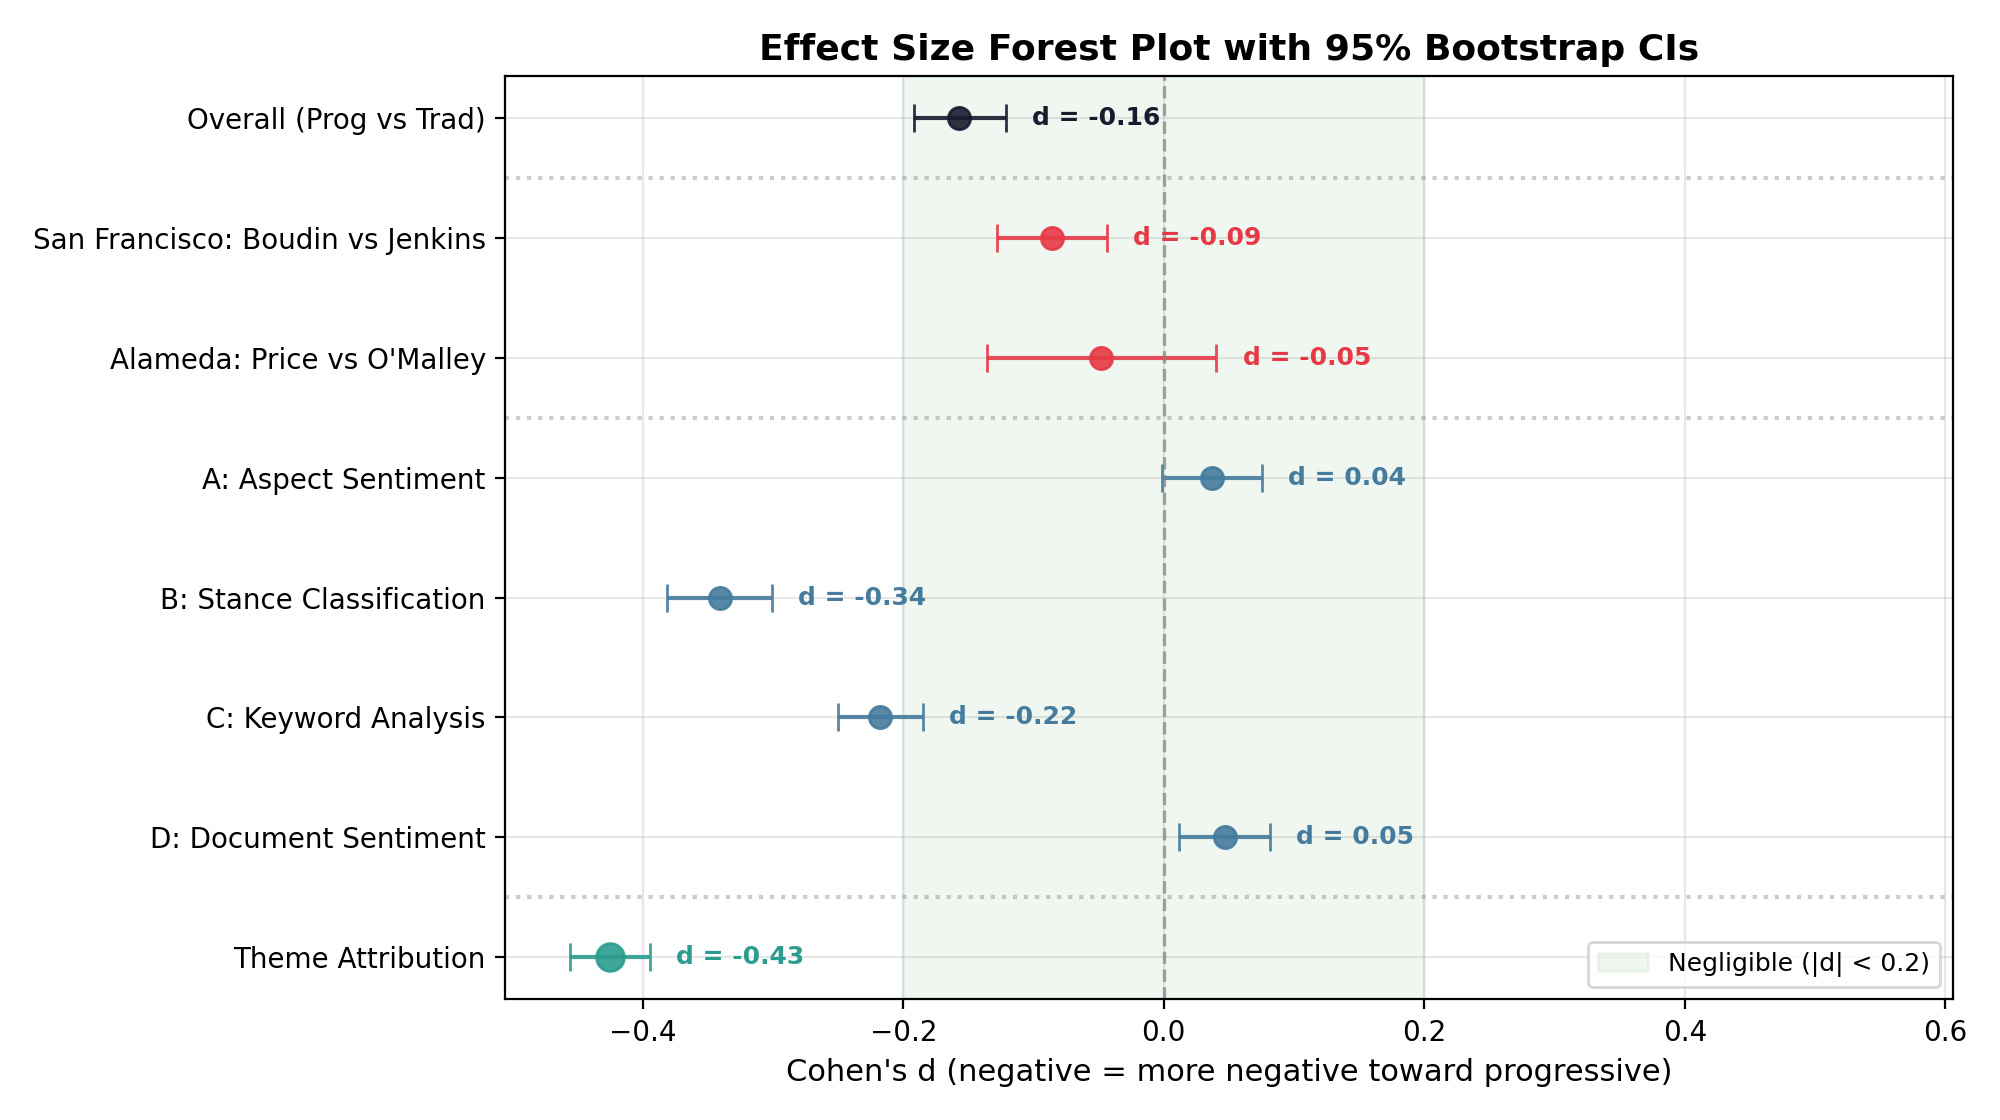
\includegraphics[width=0.85\textwidth]{06_forest_plot.png}
  \caption{Effect size forest plot with 95\% bootstrap confidence intervals. The green band marks the negligible effect zone ($|d| < 0.2$). Results are grouped by analysis type: overall, paired-county, per-method, and theme attribution. Theme attribution ($d = -0.42$) is the study's largest effect.}
  \label{fig:forest}
\end{figure}

\subsection{Same-County Paired Comparisons by Method}

The within-county design provides the strongest quasi-experimental identification. Per-method analysis reveals \emph{which dimensions} of coverage differ within each jurisdiction:

\emph{San Francisco (Boudin vs.\ Jenkins).} Stance classification detects significant differential treatment ($d = -0.197$, $p < .001$) and keyword analysis confirms it ($d = -0.093$, $p < .001$). Aspect sentiment ($d = 0.058$, $p = .020$) and document sentiment ($d = 0.069$, $p = .002$) show small \emph{reversed} (positive) differences. The bias is evaluative, not tonal.

\emph{Alameda County (Price vs.\ O'Malley).} On a composite measure, this pair shows a non-significant difference ($d = -0.069$, $p = .138$), an apparent null. However, decomposition by method reveals that the null is an artifact of aggregation: stance classification ($d = -0.272$, $p < .001$) and keyword analysis ($d = -0.381$, $p < .001$) both detect substantial differential treatment, while sentiment ($d = 0.045$, $p = .381$) and document tone ($d = 0.105$, $p = .017$) pull in the \emph{opposite} direction. The composite averages these opposing signals into a near-zero result, masking real differential treatment that operates through evaluative framing.

\begin{table}[ht]
\centering
\caption{Per-method Cohen's $d$ for same-county paired comparisons. Significant results ($p < .05$) in bold.}
\label{tab:pairedmethod}
\begin{tabular}{lrrrr}
\toprule
& \multicolumn{2}{c}{San Francisco} & \multicolumn{2}{c}{Alameda} \\
\cmidrule(lr){2-3} \cmidrule(lr){4-5}
Method & $d$ & $p$ & $d$ & $p$ \\
\midrule
B: Stance           & $\mathbf{-0.197}$ & $< .001$ & $\mathbf{-0.272}$ & $< .001$ \\
C: Keywords          & $\mathbf{-0.093}$ & $< .001$ & $\mathbf{-0.381}$ & $< .001$ \\
A: Aspect sentiment  & $\mathbf{0.058}$  & $.020$   & $0.045$           & $.381$   \\
D: Document sentiment & $\mathbf{0.069}$ & $.002$   & $\mathbf{0.105}$  & $.017$   \\
\midrule
Composite            & $\mathbf{-0.068}$ & $.002$   & $-0.069$          & $.138$   \\
\bottomrule
\end{tabular}
\end{table}

Figure~\ref{fig:perprosecutor} displays per-prosecutor mean composite scores with 95\% confidence intervals. Figure~\ref{fig:paired} presents the paired county comparisons.

\begin{figure}[H]
  \centering
  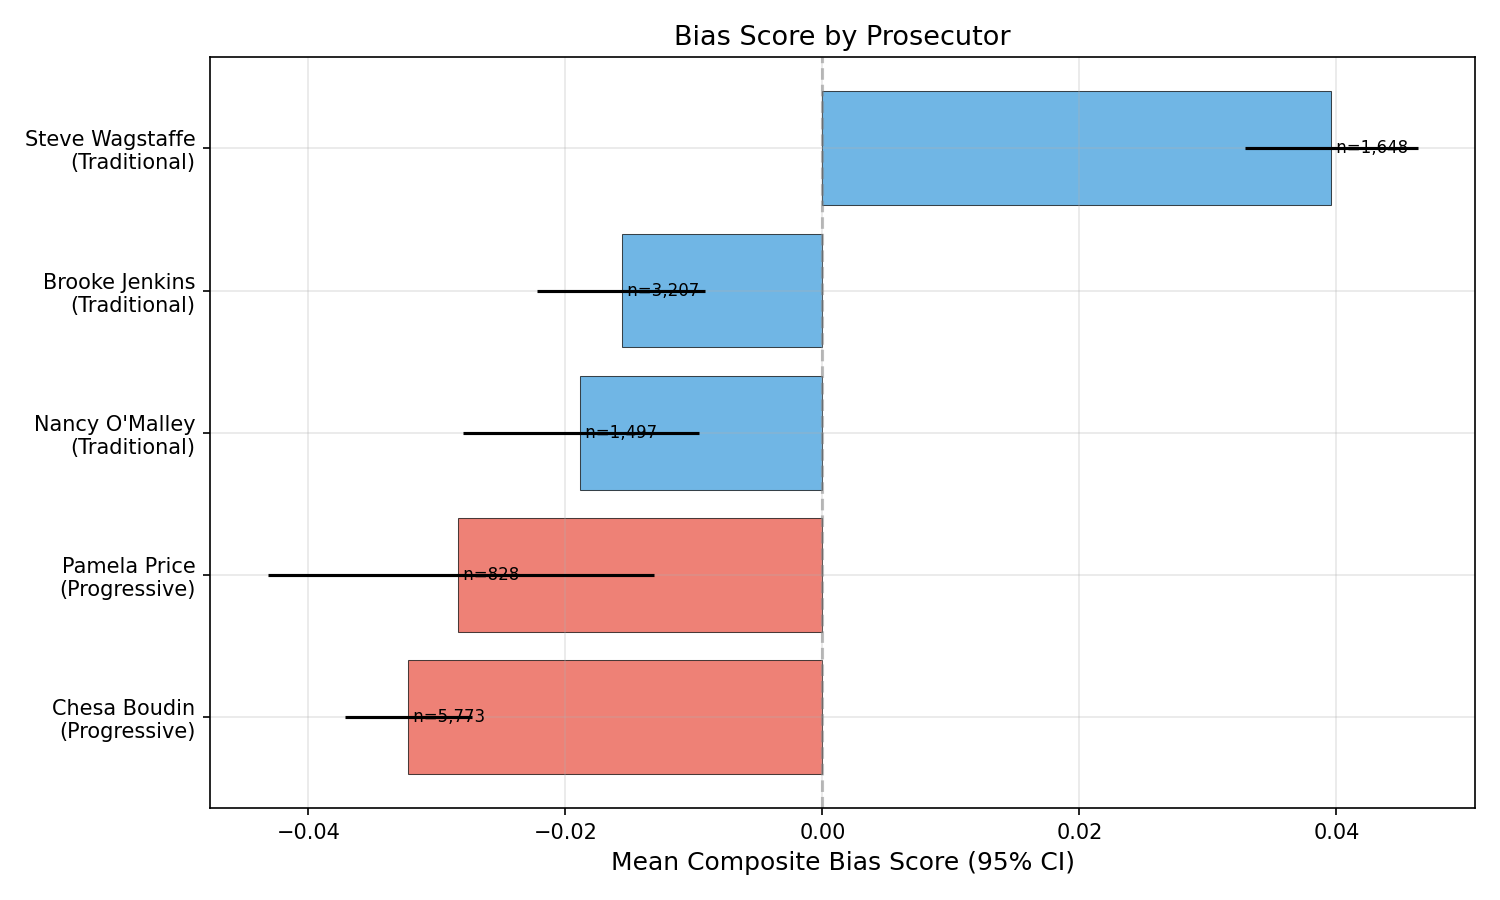
\includegraphics[width=0.85\textwidth]{02_per_prosecutor.png}
  \caption{Mean aggregate tone-evaluation index by prosecutor with 95\% confidence intervals. Red bars indicate progressive prosecutors; blue bars indicate traditional prosecutors.}
  \label{fig:perprosecutor}
\end{figure}

\begin{figure}[H]
  \centering
  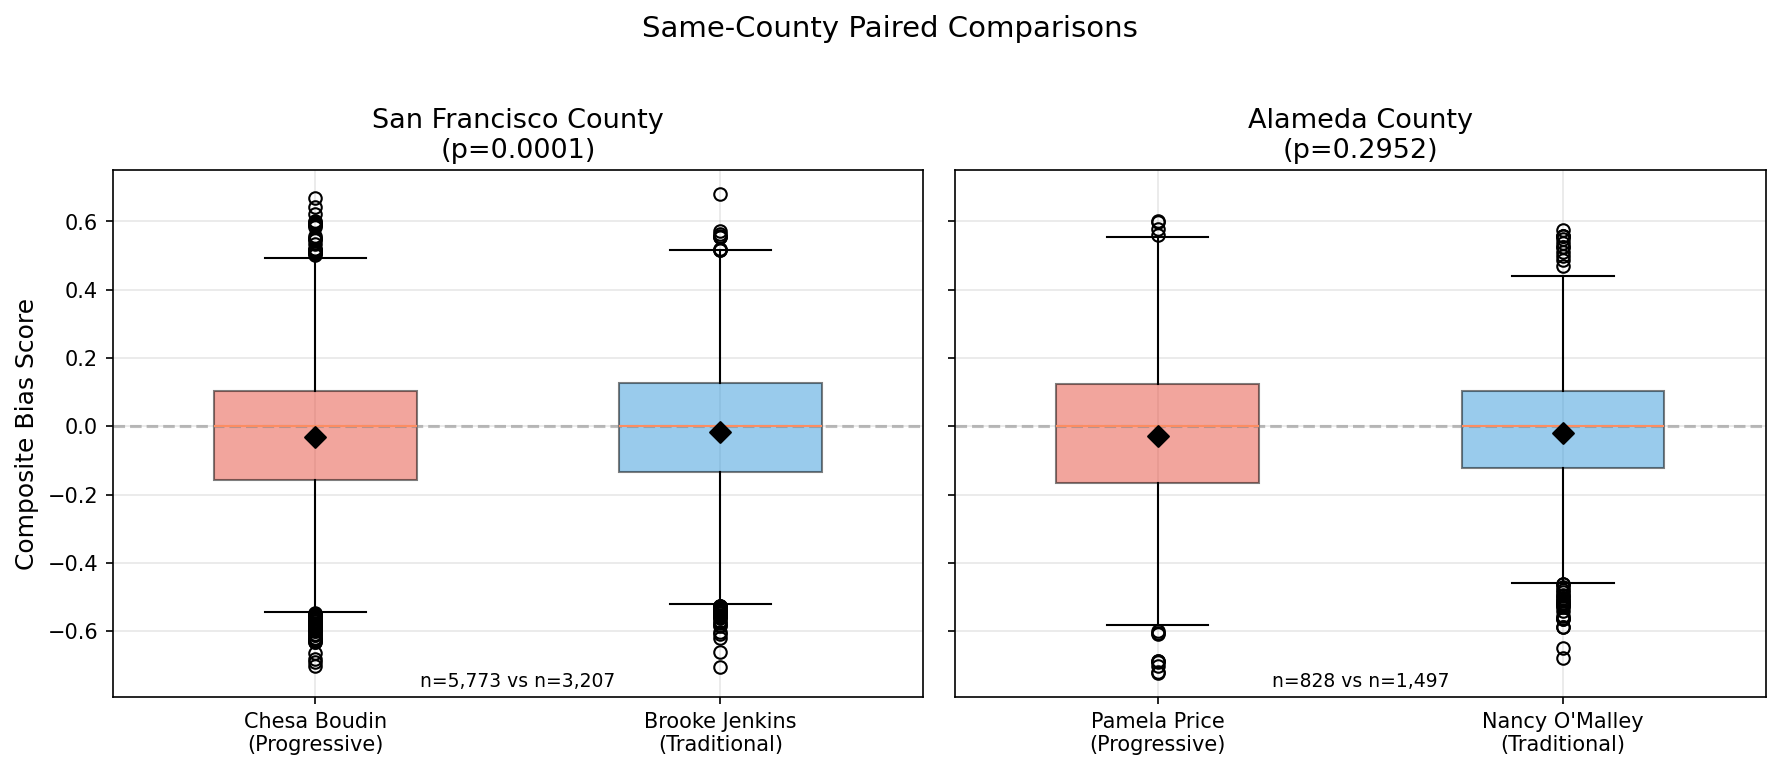
\includegraphics[width=0.9\textwidth]{03_paired_county.png}
  \caption{Same-county paired comparisons: San Francisco (Boudin vs.\ Jenkins) and Alameda (Price vs.\ O'Malley). Diamond markers indicate group means.}
  \label{fig:paired}
\end{figure}

\subsection{Regression Analysis by Method}

To test whether each bias dimension survives controls for county, year, article length, and publication clustering, I estimate separate OLS regressions for each method (Figure~\ref{fig:methodreg}; full coefficient table in Appendix~\ref{app:diagnostics}).

Stance classification and keyword analysis, the evaluative and thematic dimensions, both show significant progressive coefficients that survive all controls. Aspect sentiment and document sentiment do not. The composite regression falls to non-significance ($p = .104$) precisely because it averages the strong evaluative signal with the null tonal signal. Running regressions per method resolves this: evaluative bias is robust to controls; tonal bias does not exist.

\begin{figure}[H]
  \centering
  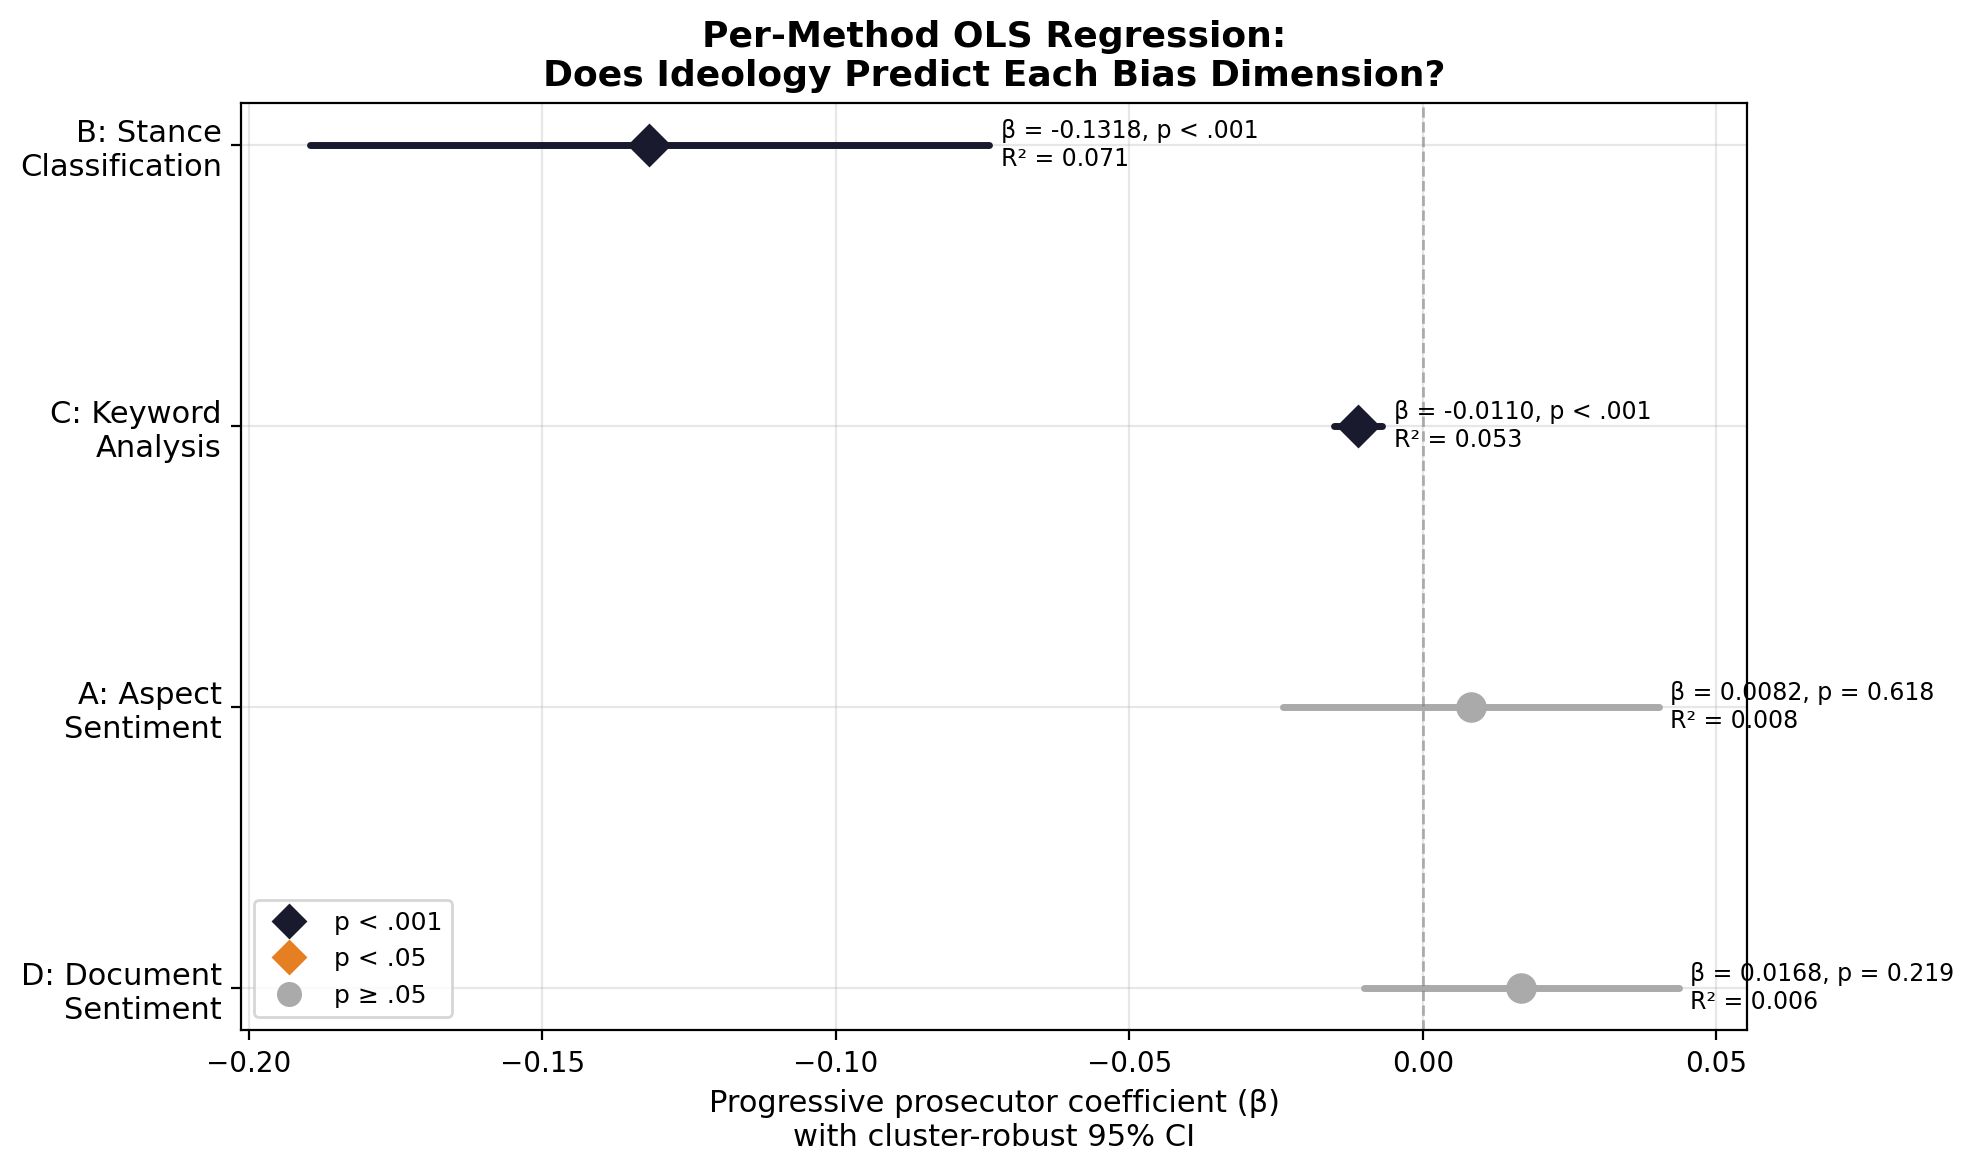
\includegraphics[width=0.85\textwidth]{16_per_method_regression.png}
  \caption{Per-method OLS regression: progressive prosecutor coefficient with 95\% cluster-robust CIs. Stance and keyword methods survive controls; sentiment methods do not.}
  \label{fig:methodreg}
\end{figure}

\subsection{Temporal Dynamics by Method}

Per-method temporal analysis combines segmented interrupted time-series modeling with quarterly decomposition to test whether the evaluative bias identified above is stable or event-driven (Figure~\ref{fig:methodtemporal}).

\emph{Segmented interrupted time series.} Monthly segmented models estimate transition-date level changes and post-transition slope changes for each outcome (Appendix~\ref{app:segmented_its}, Table~\ref{tab:segmented_its}, Figure~\ref{fig:segmented_its}). In San Francisco, the composite shows a modest positive level shift that does not reach significance ($p = .070$) and a nominally significant positive post-transition slope, consistent with movement toward less negative coverage after the Boudin-to-Jenkins transition. In Alameda, the composite and stance outcomes show immediate negative level shifts at the O'Malley-to-Price transition with little compensating slope change, consistent with a step increase in critical evaluative coverage. These composite-level ITS coefficients should, however, be read as suggestive: after Benjamini--Hochberg correction across the full 30-test ITS family, the San Francisco composite slope change and the Alameda composite level and 12-month horizon effects are no longer significant, whereas the stance and keyword effects in both counties, and the San Francisco composite 12-month horizon effect, largely survive correction (Appendix~\ref{app:segmented_its}). A controlled specification that differences each treated county against San Mateo County (Steve Wagstaffe), which experienced no prosecutor transition, confirms the Alameda level shift ($p = .003$) but not the San Francisco one ($p = .26$; Appendix~\ref{app:segmented_its}). Across transitions, evaluative measures (especially stance, then keywords) carry the temporal signal, whereas sentiment measures remain weak and inconsistent.

\emph{Quarterly heterogeneity.} Figure~\ref{fig:methodtemporal} decomposes the temporal patterns of each method across 21 quarters. Stance classification ($SD = 0.32$, range $[-0.66, +0.30]$) and keyword analysis ($SD = 0.36$, range $[-0.86, +0.54]$) show dramatic quarterly variation, with the deepest effects coinciding with the Boudin recall (2021Q4--2022Q2) and the Price recall movement (2023Q2--Q3). Aspect sentiment ($SD = 0.28$, range $[-0.32, +0.77]$) and document sentiment ($SD = 0.22$, range $[-0.15, +0.69]$) show less variation and no systematic pattern tied to political events. The monthly time series (Figure~\ref{fig:timeseries}) overlays a coverage-volume-weighted three-month rolling average alongside the raw monthly means; the weighted and unweighted trends are nearly identical, confirming that the temporal patterns are not artifacts of high-variance low-coverage months.

This per-method temporal decomposition resolves a key ambiguity in the aggregate analysis. The composite quarterly $d$ (range $[-0.38, +0.86]$, $SD = 0.39$) appears to show dramatic cyclical variation, but this aggregate masks the distinct temporal signatures of its component methods. Evaluative bias (stance, keywords) is event-driven, surging during recall campaigns and subsiding between them. Tonal bias (sentiment) is absent throughout. The aggregate temporal variation is driven entirely by the evaluative dimensions.

\begin{figure}[H]
  \centering
  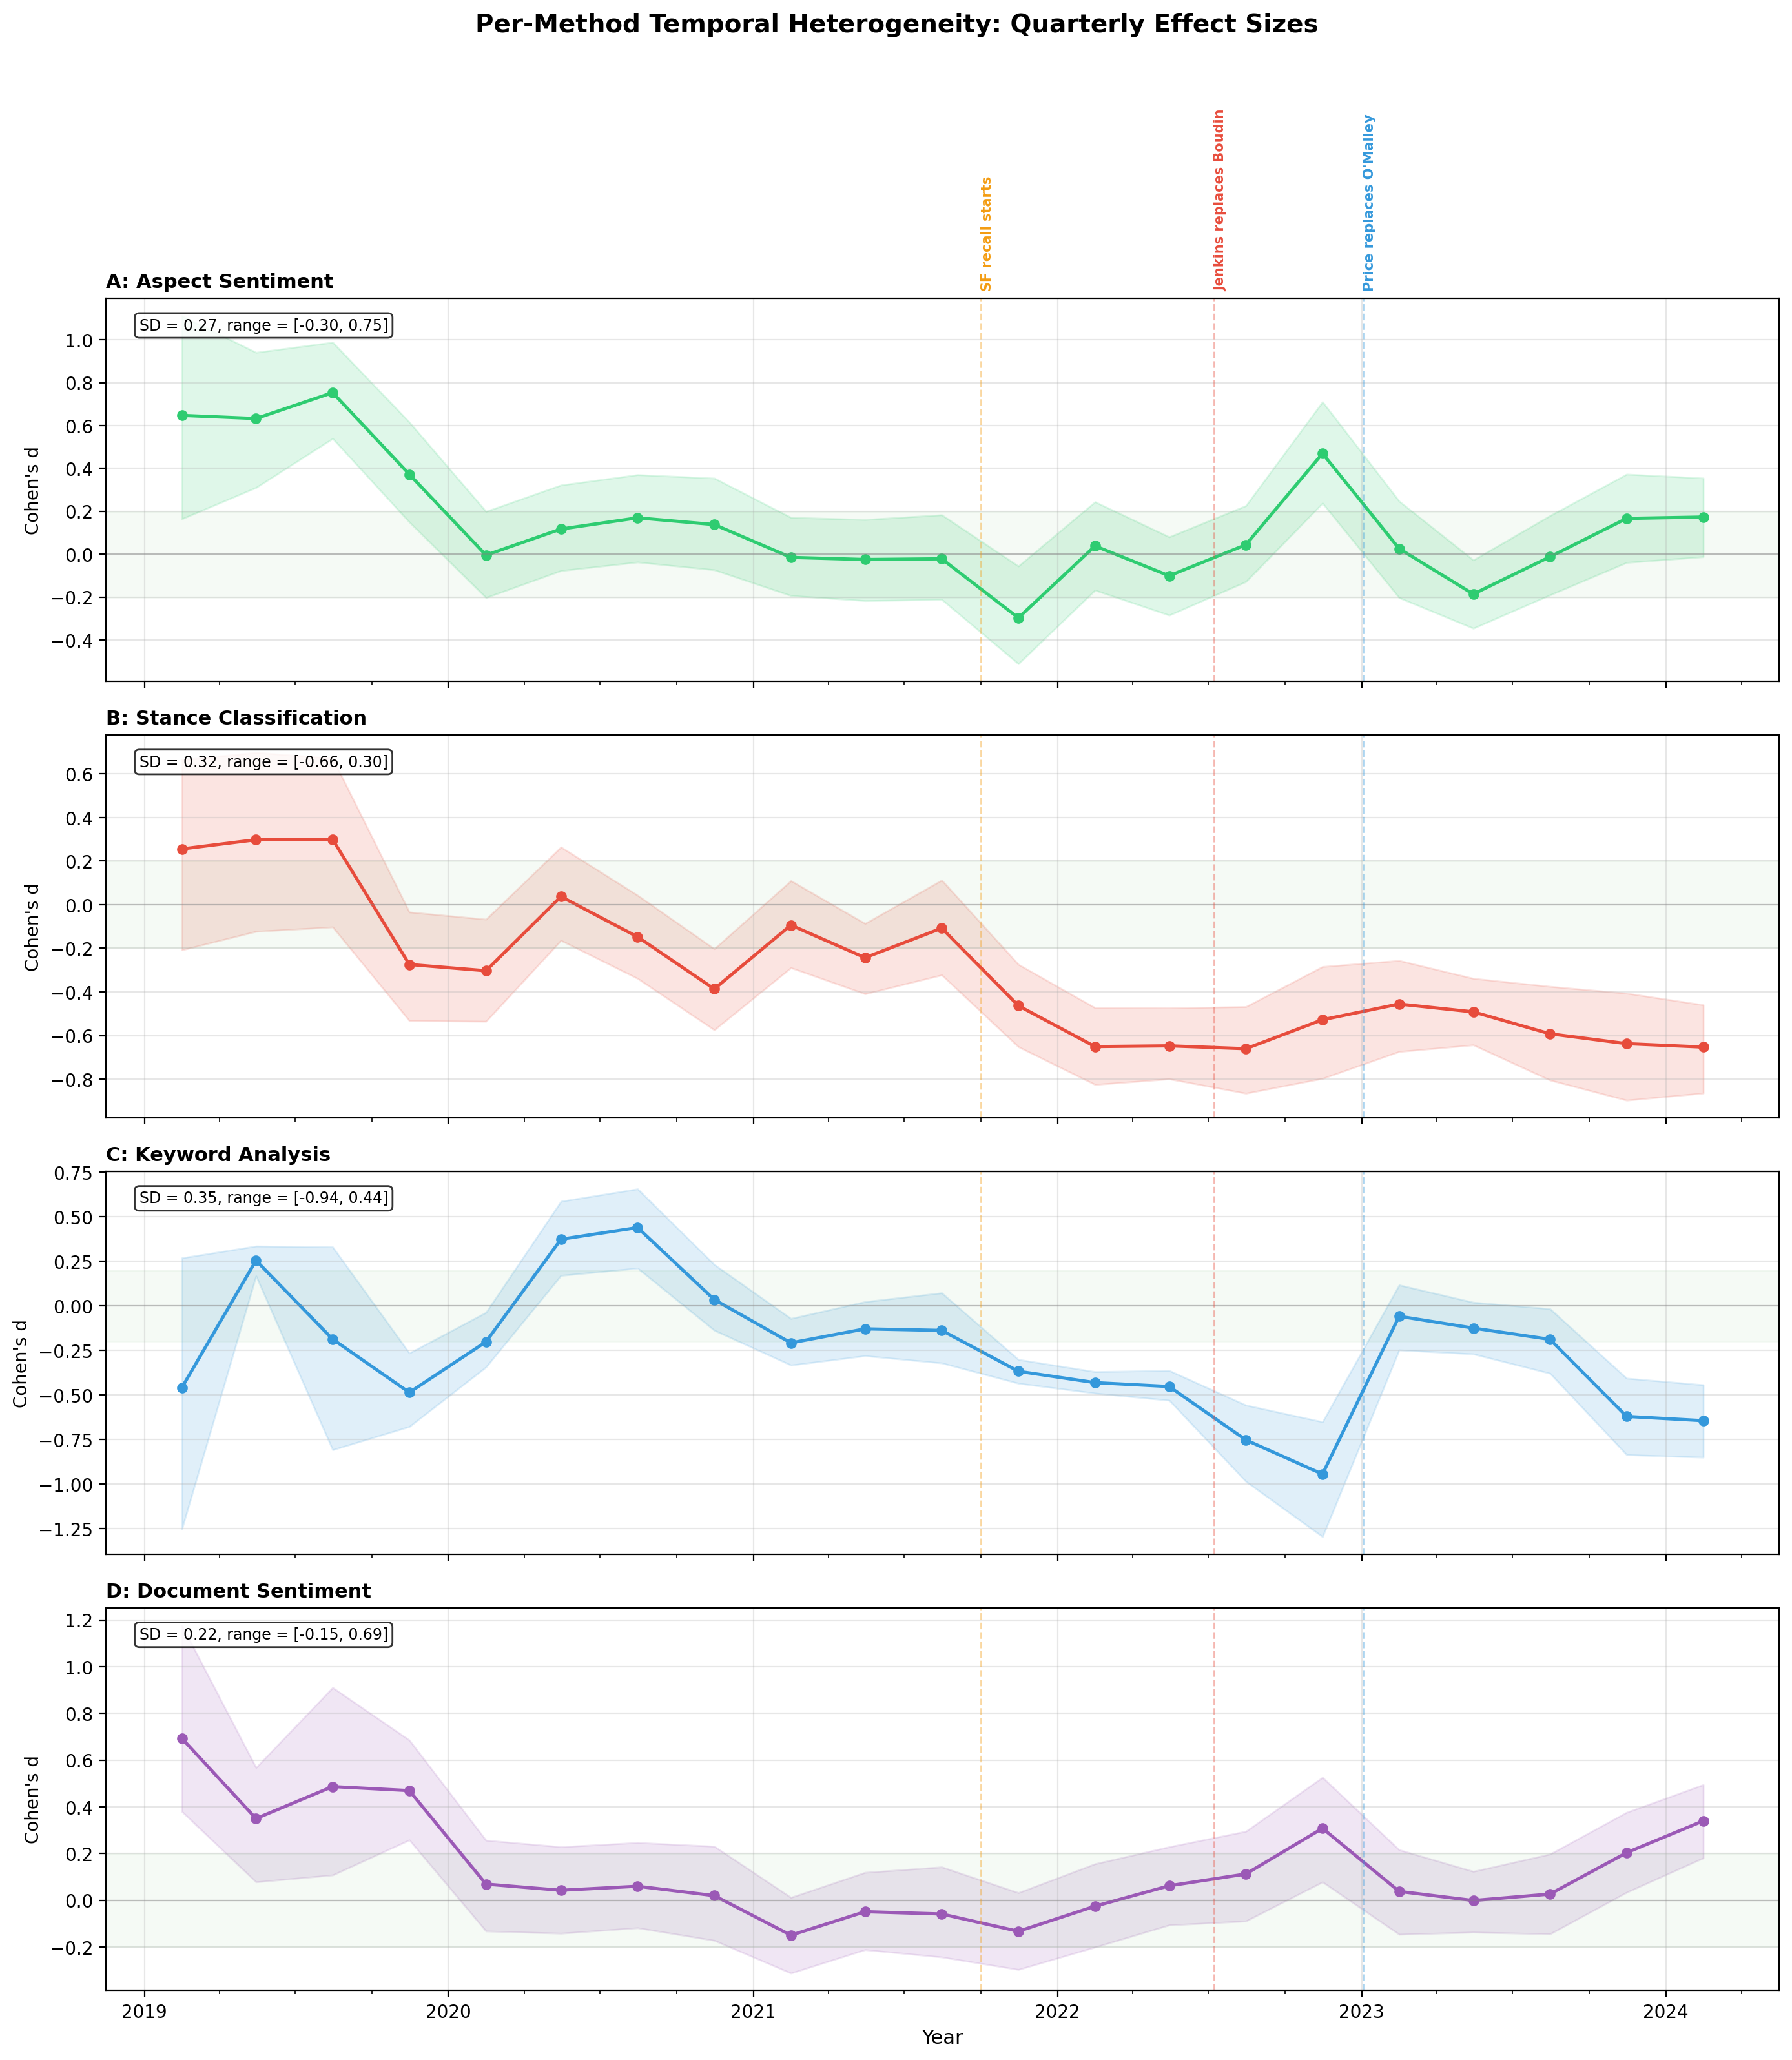
\includegraphics[width=0.95\textwidth]{17_per_method_temporal.png}
  \caption{Per-method quarterly Cohen's $d$ (progressive vs.\ traditional) with 95\% bootstrap CIs. The green band marks the negligible zone ($|d| < 0.2$). Dashed lines mark prosecutor transitions. Stance and keyword methods show event-driven variation; sentiment methods remain flat throughout.}
  \label{fig:methodtemporal}
\end{figure}

\begin{figure}[H]
  \centering
  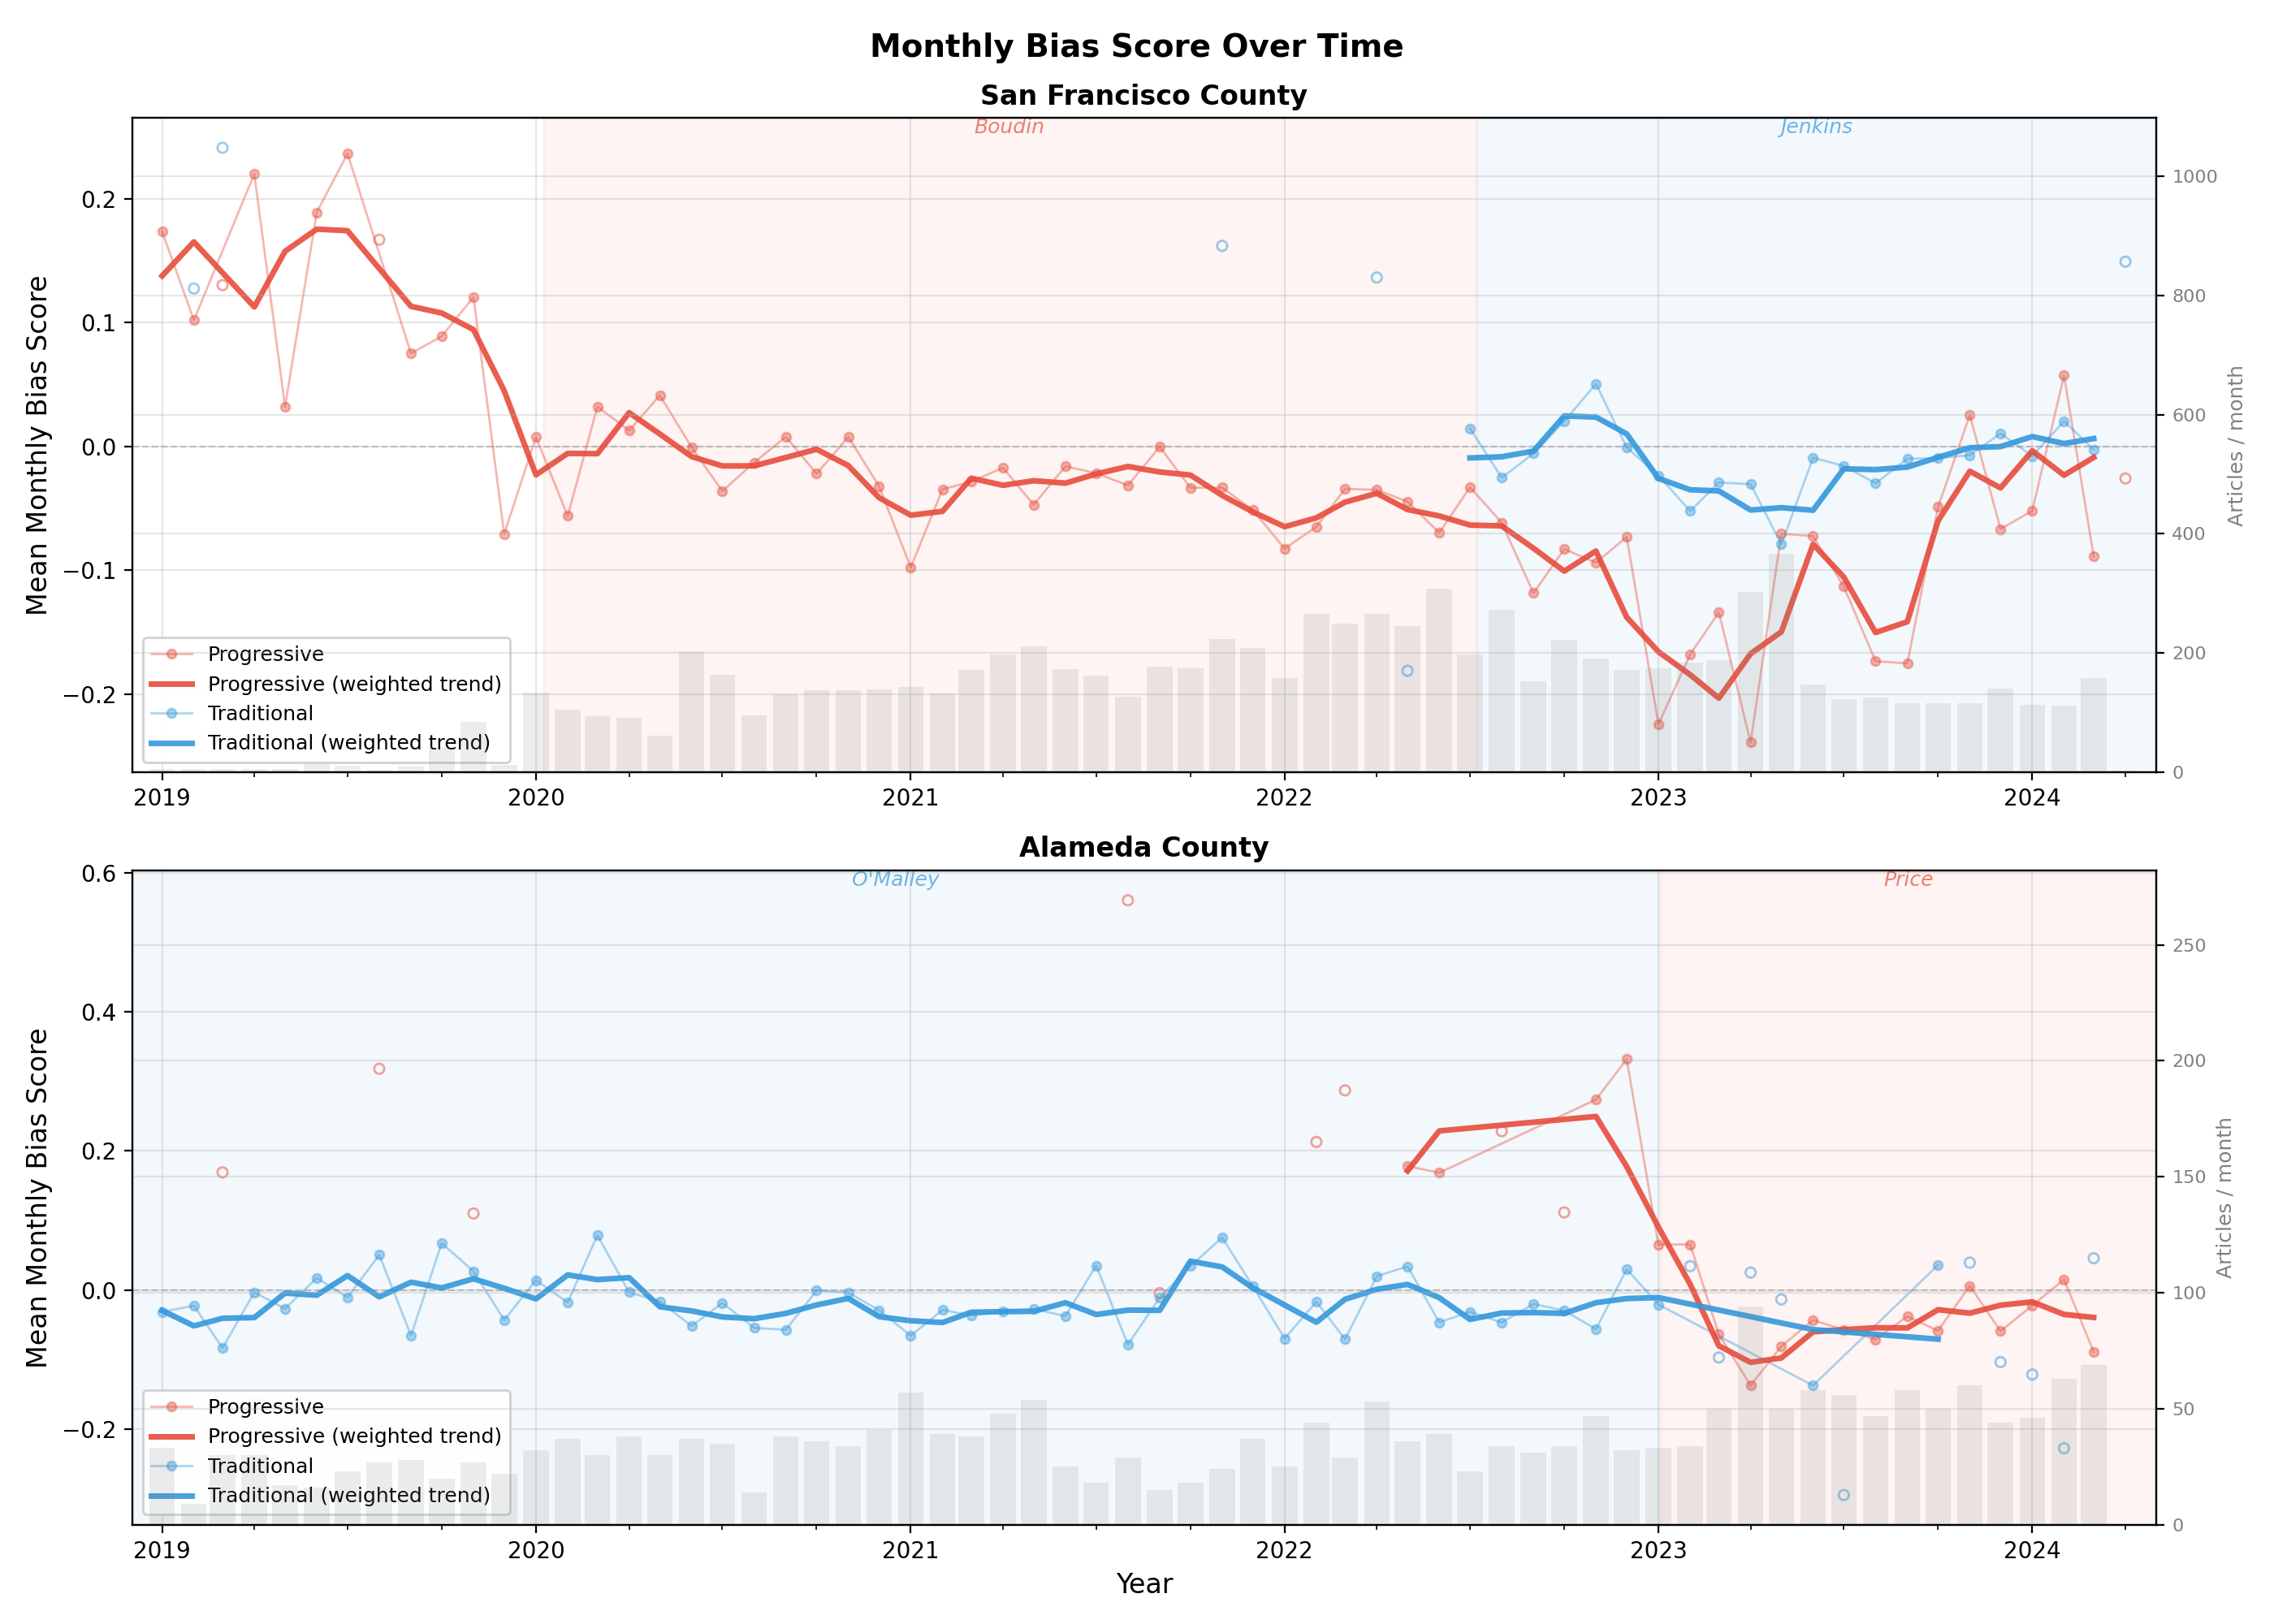
\includegraphics[width=0.95\textwidth]{04_time_series.png}
  \caption{Monthly mean composite scores for San Francisco (top) and Alameda County (bottom), 2019--2024. Faint dots and lines show raw monthly means; thick lines show coverage-volume-weighted three-month rolling averages. Open circles mark months with fewer than five articles. Shaded bands indicate prosecutor tenures; red = progressive, blue = traditional.}
  \label{fig:timeseries}
\end{figure}

\subsection{Composite Summary}

The preceding A--D analyses constitute the study's primary findings and demonstrate that evaluative and tonal dimensions of coverage diverge sharply. The composite below is reported immediately afterward because it is constructed only from Methods A--D and serves as a summary measure for overall comparison and time-series visualization, not as the principal test of differential treatment.

When the four methods are combined into a weighted composite (weights: 0.35 sentiment, 0.30 stance, 0.20 keywords, 0.15 document), the overall group comparison yields $d = -0.151$ ($p < .001$; 95\% bootstrap CI for the raw mean difference $[-0.035, -0.022]$), with a TOST equivalence test confirming the effect falls within conventional equivalence bounds ($p = .003$ at $d = 0.2$; see Section~\ref{sec:methods} for bound justification). Because articles cluster within outlets, I also re-estimate the group contrast with a publication-cluster bootstrap that resamples the 20 outlets with replacement: the 95\% CI for the raw mean difference is $[-0.0475, -0.0074]$, with a two-sided bootstrap $p \approx .011$. The contrast therefore survives outlet-level dependence, though the evidence is far less extreme than the article-level i.i.d.\ $p$-value suggests. The composite is also insensitive to quoted speech: a sensitivity variant that masks keyword matches inside quotations (Method~C's channel) yields an essentially identical estimate ($d = -0.151$, $p < .001$). Across the seven alternative weighting specifications reported in the Methods section, the composite differential ranges from $d = -0.282$ (evaluative methods only) to $d = +0.025$ (dropping stance; $p = .15$): the composite is negative and significant under every scheme that retains the stance method, but the differential vanishes when stance is removed, consistent with the per-method finding that the bias is evaluative rather than tonal. This composite serves as a proxy for the aggregate reader experience: a reader does not consume ``stance'' and ``sentiment'' as separate channels but is exposed to both the emotional tone and the evaluative framing of an article simultaneously. The composite approximates this net impression and provides a single dependent variable for the time series and overall comparison (Figure~\ref{fig:violin}). However, the per-method results above demonstrate that this aggregate figure obscures the distinct mechanisms at play: it averages a large evaluative effect with a null tonal effect, producing a small overall number that understates the stance differential and overstates the sentiment contribution.

\begin{figure}[H]
  \centering
  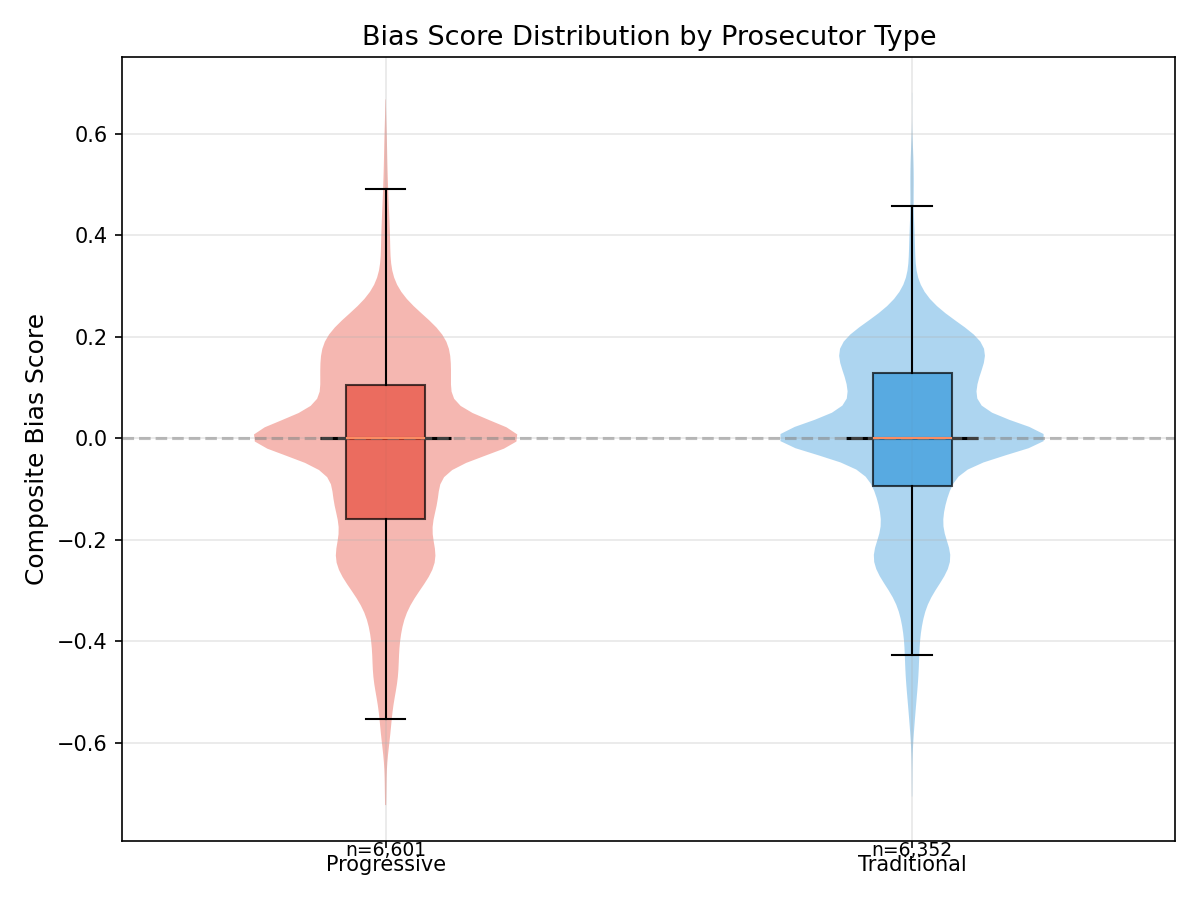
\includegraphics[width=0.75\textwidth]{01_violin_by_type.png}
  \caption{Aggregate tone-evaluation index distributions by prosecutor ideology. Violin plots show the full distribution; inner box plots show the interquartile range. Negative scores indicate more negative coverage.}
  \label{fig:violin}
\end{figure}

\subsection{Framing Analysis}

The distribution of dominant media frames differs significantly between progressive and traditional prosecutors, $\chi^2(4) = 395.66$, $p < .001$, Cram\'{e}r's $V = 0.214$ (see Figure~\ref{fig:heatmap}):

\begin{table}[ht]
\centering
\caption{Dominant media frame distribution by prosecutor ideology.}
\label{tab:frames}
\begin{tabular}{lrr}
\toprule
Frame & Progressive & Traditional \\
\midrule
Accountability & 41.1\% & 24.6\% \\
Conflict       & 29.8\% & 36.6\% \\
Human interest & 21.4\% & 33.6\% \\
Reform         &  4.2\% &  1.2\% \\
Consequences   &  3.5\% &  3.9\% \\
\bottomrule
\end{tabular}
\end{table}

Progressive prosecutors are nearly twice as likely to be covered through an accountability frame (41.1\% vs.\ 24.6\% of articles; Cohen's $h = 0.35$) and more than three times as likely through a reform frame (4.2\% vs.\ 1.2\%, $h = 0.19$). Conversely, traditional prosecutors receive substantially more human-interest framing as the dominant frame (33.6\% vs.\ 21.4\%, $h = -0.27$): stories organized around individual victims, defendants, or community members rather than evaluations of prosecutorial performance. Traditional prosecutors are also somewhat more likely to receive conflict as the dominant frame (36.6\% vs.\ 29.8\%, $h = -0.15$), while dominant consequences framing is rare and essentially equal across groups (3.5\% vs.\ 3.9\%, $h = -0.02$). The continuous frame probability scores tell a complementary story: progressive coverage scores significantly higher on accountability ($d = 0.133$, $p < .001$), reform ($d = 0.269$, $p < .001$), consequences ($d = 0.174$, $p < .001$), and even conflict ($d = 0.074$, $p < .001$), while human-interest probabilities do not differ significantly ($d = 0.001$, $p = .973$). In the full (hybrid) sample the probability-score and assignment-rate results therefore diverge in sign for the human-interest and conflict frames. Rate effect sizes are Cohen's $h$ on per-frame dominant-frame assignment rates, matching the proportions in Table~\ref{tab:frames}; the $d$ values refer to the underlying frame probability scores. All four significant frame-probability contrasts remain significant after Benjamini--Hochberg correction across the five-frame family.

Because half of the frame rows come from the keyword fallback rather than the zero-shot classifier, I rerun the framing analyses restricted to the 6{,}175 model-classified articles. Every differential strengthens on this subset --- $\chi^2(4) = 492.1$, Cram\'{e}r's $V = 0.282$; accountability $d = 0.249$, reform $d = 0.607$, consequences $d = 0.216$ --- and the two anomalies in the hybrid sample resolve: human-interest probabilities are now strongly \emph{higher} for traditional prosecutors ($d = -0.413$, $p < 10^{-59}$) and conflict probabilities flip to the traditional direction ($d = -0.119$, $p < .001$), so that all five probability-score contrasts align in sign with the dominant-frame assignment rates. The rate-versus-probability divergence in the full sample is thus attributable to the keyword fallback, which attenuates group differences toward zero and distorts the human-interest and conflict contrasts. The headline hybrid-sample framing results should accordingly be read as conservative: the measurement mixture works against the framing differential, not in its favor.

These framing patterns are consistent with the stance classification finding: the media evaluates progressive prosecutors through accountability and ideological lenses while presenting traditional prosecutors through less evaluative, story-driven narratives.

\begin{figure}[H]
  \centering
  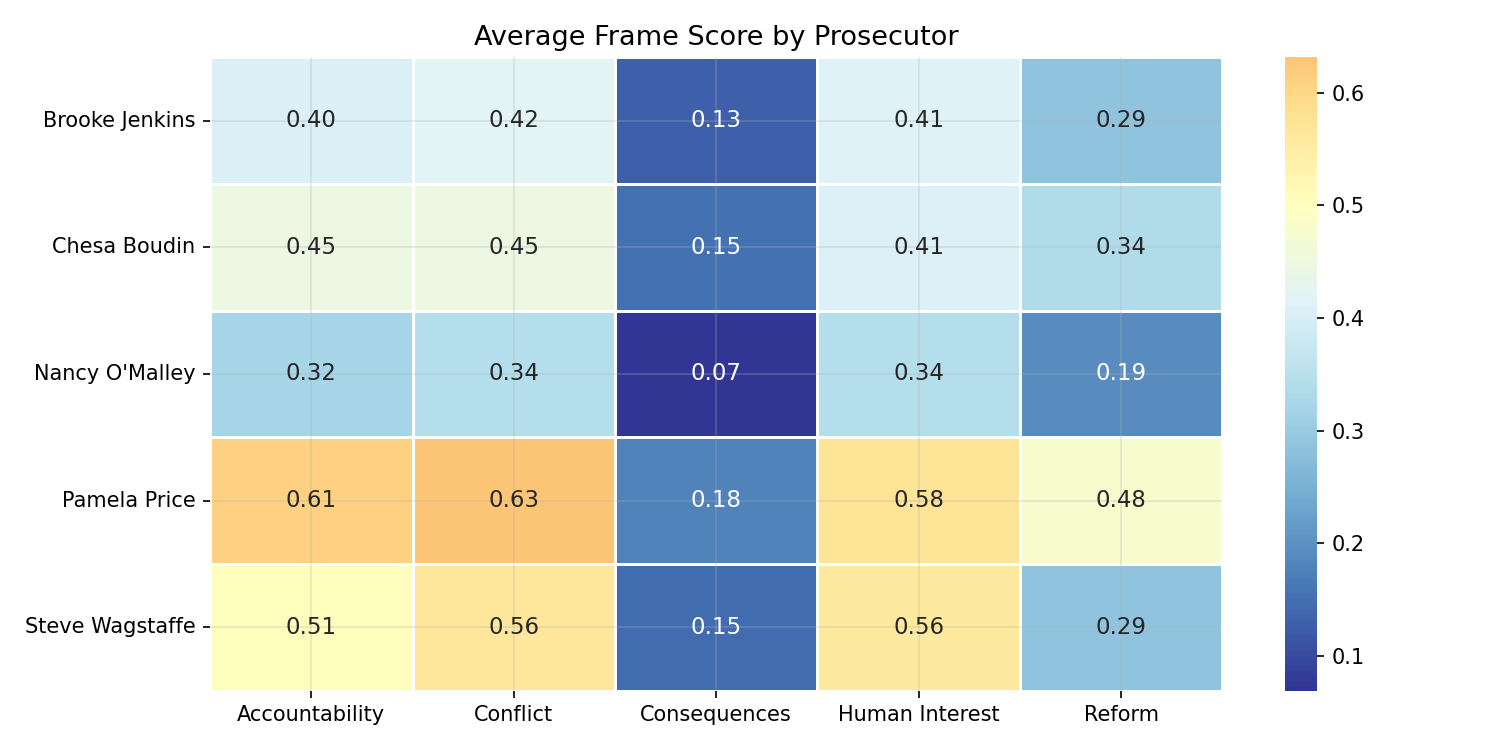
\includegraphics[width=0.8\textwidth]{05_framing_heatmap.png}
  \caption{Heatmap of average frame scores by prosecutor. Warmer colors indicate higher frame prevalence. Progressive prosecutors (Boudin, Price) score higher on accountability and reform; traditional prosecutors (Jenkins, O'Malley, Wagstaffe) score higher on human interest. Note: values represent average model probability scores, whereas Table~\ref{tab:frames} reports dominant frame assignments (the frame with the highest probability per paragraph).}
  \label{fig:heatmap}
\end{figure}

\subsection{Theme Prevalence and Prosecutor-Attributed Themes}

This subsection reports two complementary theme analyses. \emph{Part A (Method~C descriptive prevalence):} Figure~\ref{fig:themes} presents keyword prevalence from the Method~C dictionaries, measured as local term density within three-sentence windows around prosecutor mentions. By this measure, recall-related language dominates progressive prosecutor coverage (9.5\% vs.\ 2.7\% for traditional), driven overwhelmingly by Boudin's 2022 recall campaign. After recall, the most prevalent anti-prosecutor themes for progressive coverage are soft-on-crime (1.6\% vs.\ 0.7\%), public-safety-failure (1.2\% vs.\ 0.3\%), and crime-rising (0.9\% vs.\ 0.2\%). The ``releasing criminals'' theme is the only category where traditional prosecutors receive higher prevalence (5.5\% vs.\ 4.2\%), likely reflecting routine bail and parole coverage rather than ideologically targeted framing.

\begin{figure}[H]
  \centering
  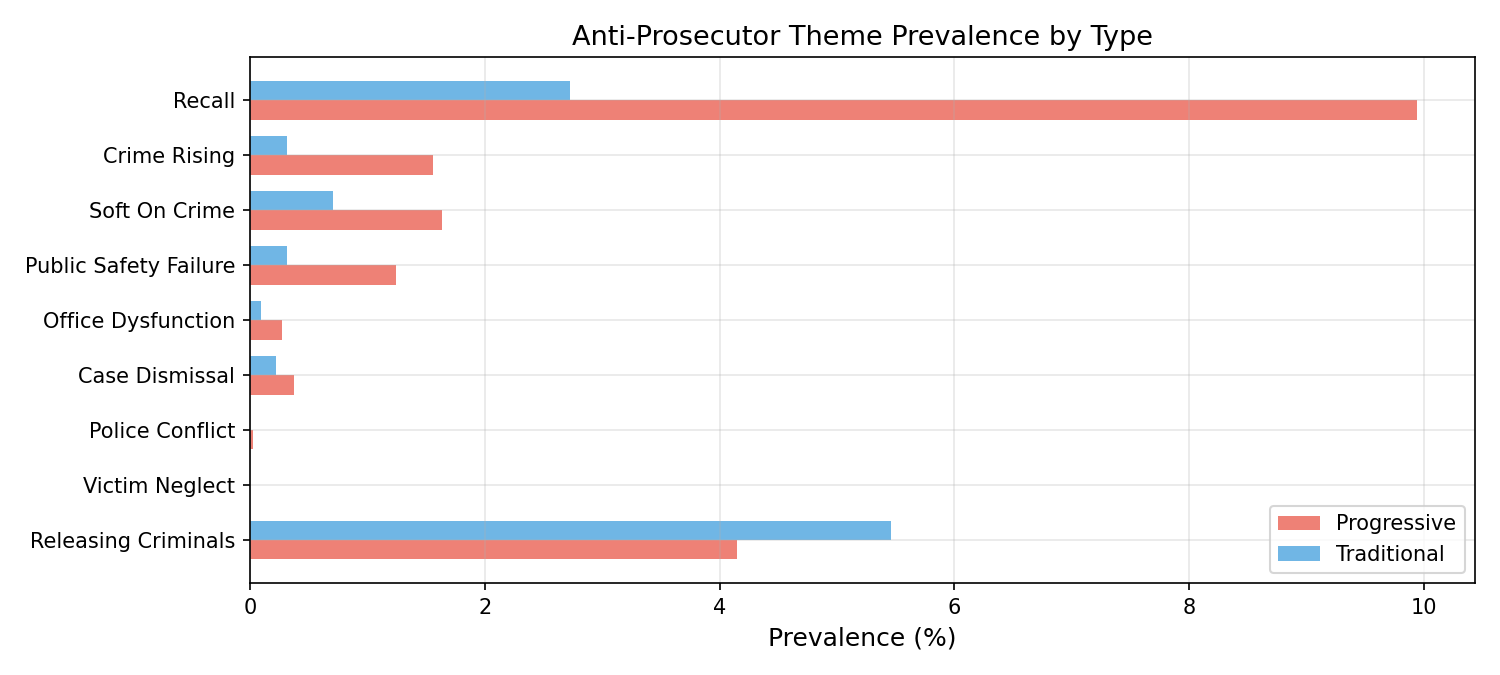
\includegraphics[width=0.85\textwidth]{07_theme_prevalence.png}
  \caption{Anti-prosecutor theme prevalence by ideology. Themes are sorted by the difference between progressive and traditional prevalence rates.}
  \label{fig:themes}
\end{figure}

\emph{Part B (prosecutor-attributed theme model):} The multi-method prosecutor-attributed theme analysis requires themes to be explicitly linked to prosecutors through compound regex patterns rather than simple keyword proximity. This stricter attribution measure provides the strongest evidence of differential thematic coverage. Progressive prosecutors receive significantly higher theme attribution scores ($M = 1.68$, $SD = 2.99$) than traditional prosecutors ($M = 0.67$, $SD = 1.65$), $t(10{,}359) = 24.01$, $p < 10^{-123}$, $d = -0.42$ (signed to match the composite convention: negative indicates more anti-prosecutor coverage), 95\% bootstrap CI for the mean difference $[0.94, 1.10]$. This medium effect size is the study's largest, exceeding the stance classification effect ($d = -0.337$) and confirming that the evaluative differential operates through the explicit attribution of critical narratives to specific prosecutors. The differential is not an artifact of quoted speech: excluding theme matches inside quotations, which restricts the comparison to the outlet's own voice, leaves the effect essentially unchanged ($d = -0.40$, $p < 10^{-115}$).

Per-theme analysis (Figure~\ref{fig:themeattr}) uses a different metric: the percentage of articles in which \emph{any} of the four attribution methods flags the theme, producing higher prevalence rates than the keyword-proximity measure above. By this article-level flag, recall-related themes appear 4.47 times more often in progressive prosecutor coverage (18.3\% vs.\ 4.1\%, $\chi^2 = 639.6$, $p < 10^{-140}$, Cram\'{e}r's $V = 0.22$). Crime-rising themes appear 1.80 times more often (20.7\% vs.\ 11.5\%, $\chi^2 = 200.1$, $p < 10^{-44}$), and soft-on-crime framing is 3.84 times more prevalent ($\chi^2 = 62.2$, $p < 10^{-14}$). Seven of the nine themes differ significantly after Benjamini--Hochberg correction across the theme family; the exceptions are releasing-criminals and the near-empty office-dysfunction category. The paired county theme comparisons confirm (reported in the standard progressive-minus-traditional direction, where positive $d$ indicates higher theme attribution for the progressive prosecutor): in San Francisco, Boudin scores higher than Jenkins ($d = 0.27$, $p < .001$), and in Alameda, Price scores higher than O'Malley ($d = 0.68$, $p < .001$), the study's largest within-county effect.

\begin{figure}[H]
  \centering
  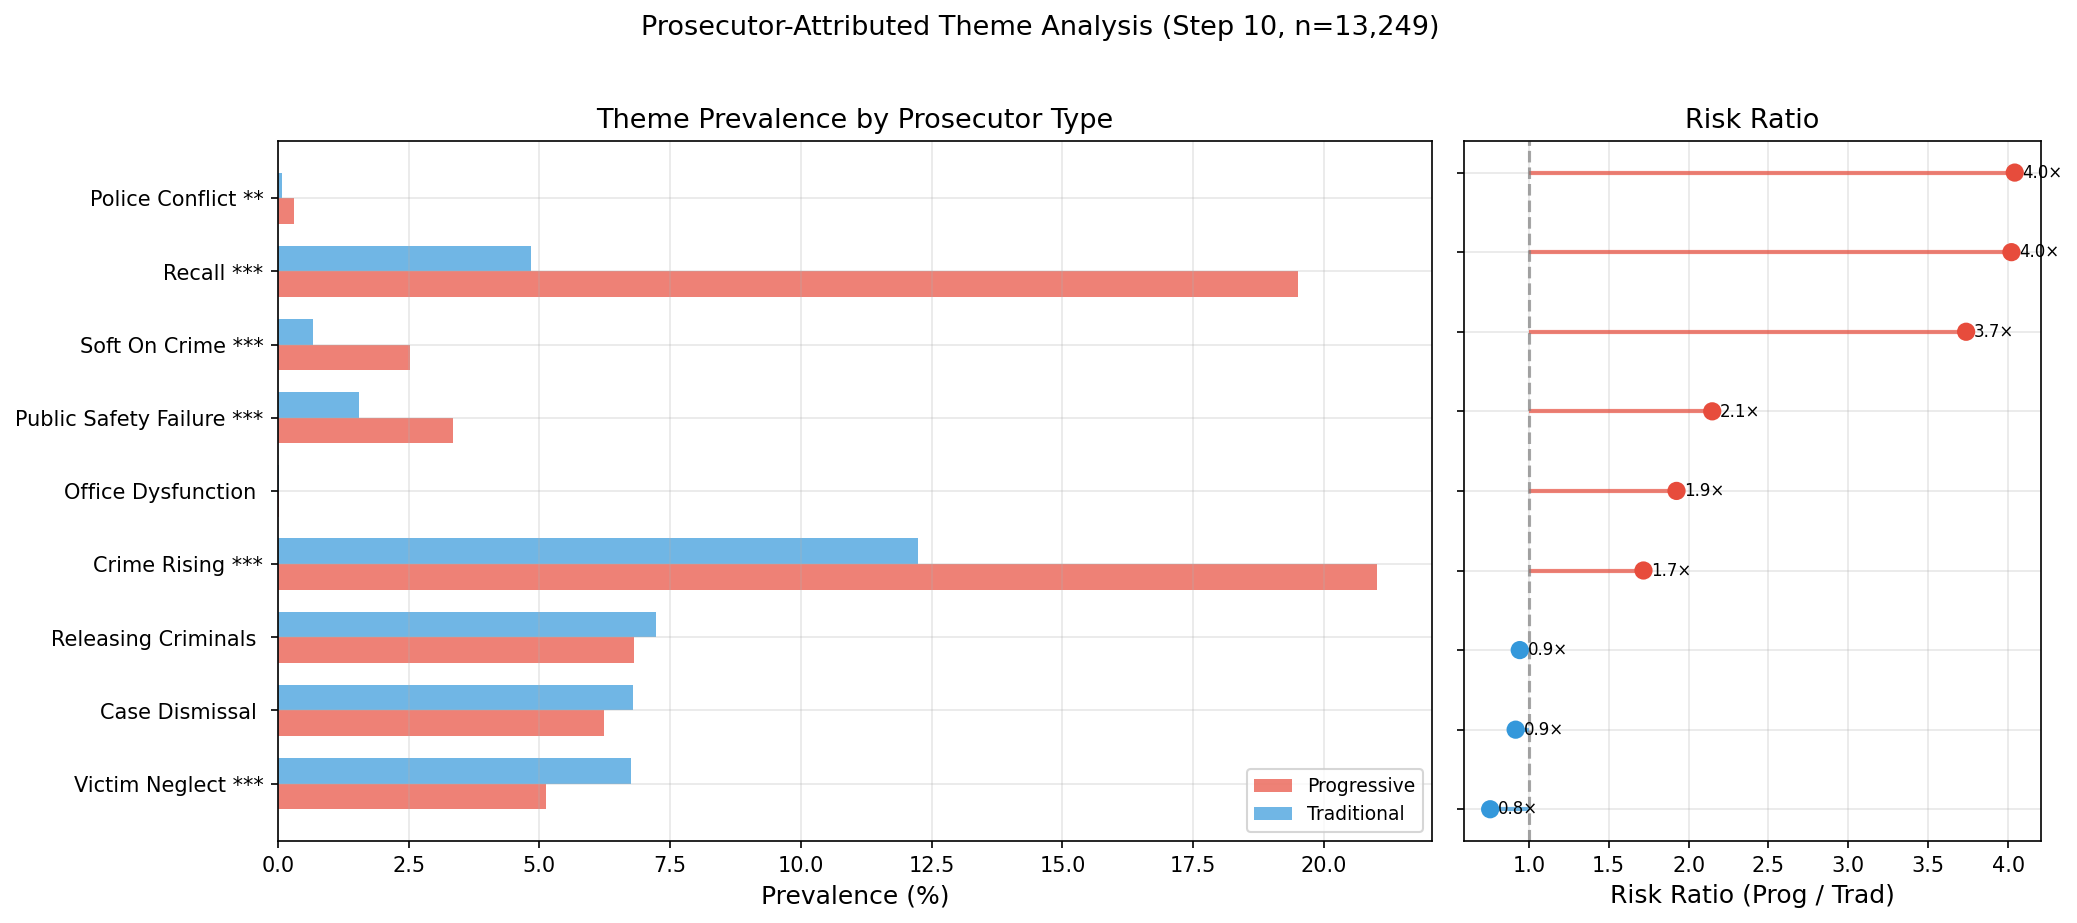
\includegraphics[width=\textwidth]{12_theme_attribution_differential.png}
  \caption{Prosecutor-attributed theme prevalence by ideology (left) and risk ratios (right). Significance: $^{***}p < .001$, $^{**}p < .01$, $^{*}p < .05$. Themes sorted by risk ratio.}
  \label{fig:themeattr}
\end{figure}

Multi-method validation shows that 38.2\% of articles with any detected theme trigger two or more independent detection methods, confirming convergent evidence rather than single-method artifacts (Appendix~\ref{app:diagnostics}).

\subsection{Structural Source Ecology and Claims (Full-Corpus LLM Extraction)}
\label{sec:structural_results}

After establishing evaluative differentials with NLP scoring, this section identifies the structural content patterns that co-occur with those differentials. Source types differ strongly by prosecutor ideology ($\chi^2(\SourceChiSqDf) = \SourceChiSq$, $p \SourceChiSqP$), with progressive prosecutor coverage drawing disproportionately on advocacy voices (\AdvocacyRatio$\times$), journalist commentary (\JournalistRatio$\times$), politicians (\PoliticianRatio$\times$), and experts (\ExpertRatio$\times$) relative to traditional coverage. Human validation of extraction recall (Section~\ref{sec:human_validation}) finds that unnamed and documentary attribution is disproportionately missed but that recall failure is symmetric across prosecutor types; the between-group ratios reported here are therefore the robust quantity, while the underlying composition understates documentary sources (see Appendix~\ref{app:extraction}).

\begin{table}[ht]
\centering
\caption{Source stance per article by prosecutor ideology (full extraction, $n=\NAttributedTotal$).}
\label{tab:sourcestance}
\small
\begin{tabular}{lrrrr}
\toprule
Source Stance & Prog./art. & Trad./art. & $d$ & Ratio \\
\midrule
Critical    & \ProgCriticalPerArticle & \TradCriticalPerArticle & $0.14$ & \CriticalRateRatio$\times$ \\
Supportive  & \ProgSupportivePerArticle & \TradSupportivePerArticle & $0.22$ & \SupportiveRateRatio$\times$ \\
Neutral     & \ProgNeutralPerArticle & \TradNeutralPerArticle & $-0.20$ & \NeutralRateRatio$\times$ \\
\bottomrule
\end{tabular}
\end{table}

Progressive prosecutors attract both more critical and more supportive source attributions per article, while traditional prosecutors receive more neutral sourcing. The largest absolute source-rate difference remains prosecutor self-quotation (\ProgSelfQuoteRate\ per article for progressives vs.\ \TradSelfQuoteRate\ for traditional), indicating that traditional coverage is more often anchored in the officeholder's own framing while progressive coverage draws more external contestation.

Causal attributions show the same directional asymmetry: ``prosecutor caused harm'' appears at \ProgHarmPerArticle\ per progressive article versus \TradHarmPerArticle\ per traditional article (\HarmRatio$\times$), while ``prosecutor helped'' also appears slightly more often for progressives (\ProgHelpedPerArticle\ vs.\ \TradHelpedPerArticle, \HelpedRatio$\times$). For claim content, policy and performance criticism show the largest differentials (policy: \ProgPolicyClaimRate\ vs.\ \TradPolicyClaimRate\ per article, \PolicyClaimRatio$\times$; performance: \ProgPerformanceClaimRate\ vs.\ \TradPerformanceClaimRate, \PerformanceClaimRatio$\times$), while character and competence claims are comparatively symmetric (\CharacterClaimRatio$\times$ and \CompetenceClaimRatio$\times$).

\begin{figure}[H]
  \centering
  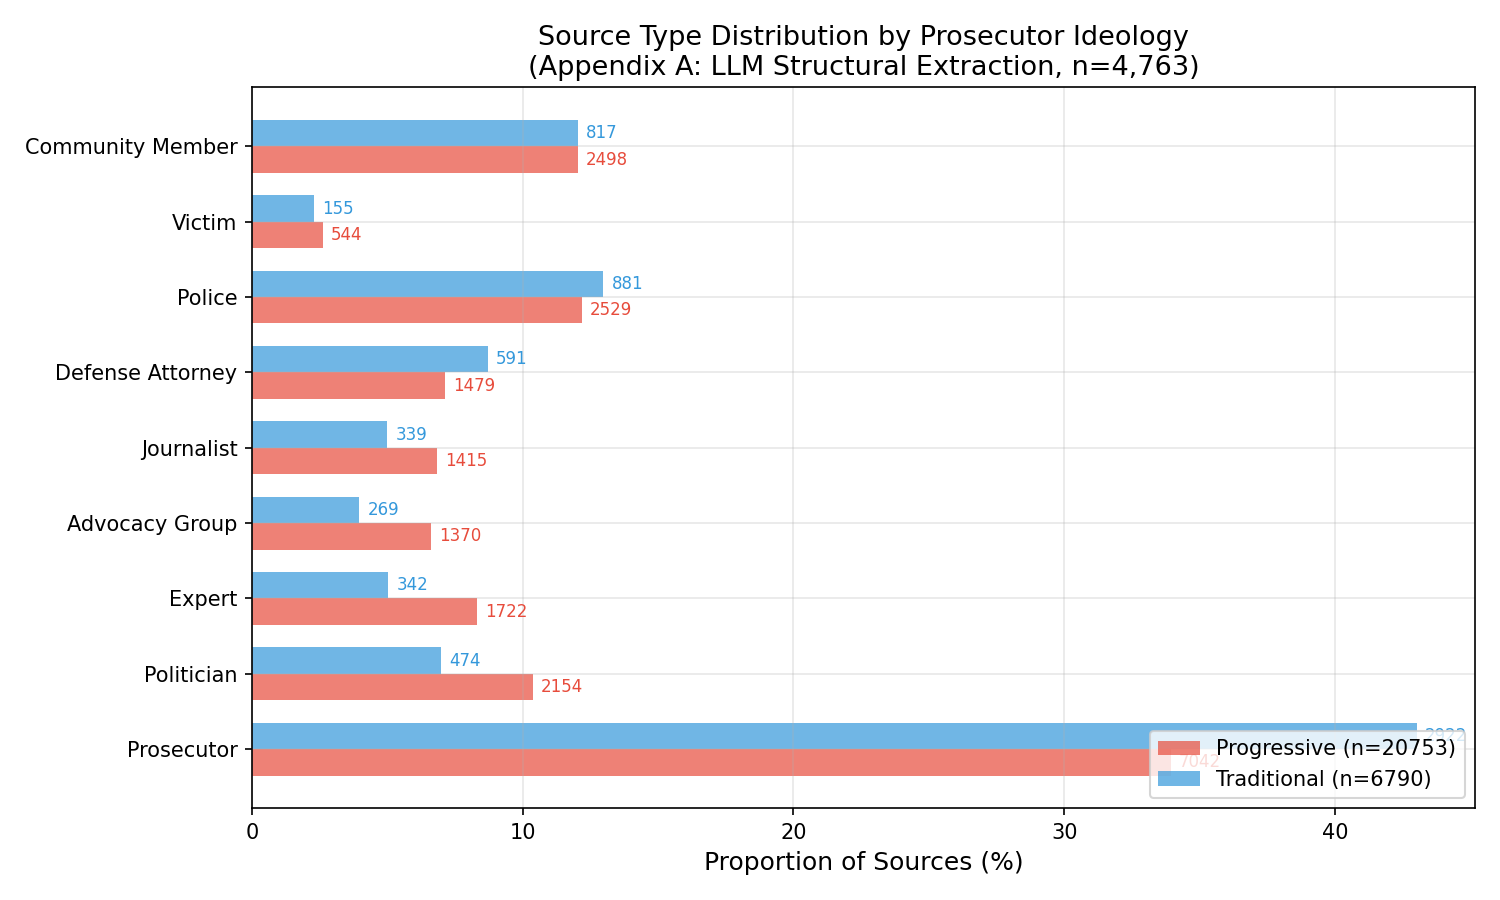
\includegraphics[width=0.85\textwidth]{08_source_type_distribution.png}
  \caption{Source type distribution by prosecutor ideology from LLM structural extraction ($n=\NAttributedTotal$ articles). Bars show proportions of total sources within each group; annotations show raw counts. The largest relative differentials are in advocacy groups (\AdvocacyRatio$\times$), journalist commentary (\JournalistRatio$\times$), politicians (\PoliticianRatio$\times$), and expert sources (\ExpertRatio$\times$).}
  \label{fig:sourcetypes}
\end{figure}

These structural patterns are consistent with the evaluative-framing findings but remain descriptive rather than causal.

Robustness checks point in the same direction: excluding Brooke Jenkins from the traditional baseline, excluding fallback-attributed articles, restricting to prosecutor-focused articles, applying a stricter mention-dominance relevance rule, and restricting to tenure-period coverage all preserve or increase effect magnitudes, indicating attenuation rather than artifact in the full-sample estimates (Appendices~\ref{app:baseline_sensitivity} and~\ref{app:fallback_sensitivity}).

\subsection{Human Validation of Automated Measures}
\label{sec:human_validation}

A trained research assistant independently coded a stratified 100-article validation sample, labeling each article's stance toward the attributed prosecutor, its dominant media frame, and whether it was substantively about that prosecutor, and audited the corresponding extraction outputs. The validation program now comprises four completed packets---the 100-article stance-and-frame sample, a 160-extraction audit, a 120-article case-type coding task, and a 40-article extraction-recall audit, covering 373 distinct articles in total. One design caveat applies throughout: the coding packets displayed the model's labels alongside the article text, so the coding was not blind to model outputs. Non-blind coding can only inflate agreement, which makes the low agreement estimates reported below conservative in the direction that matters. A second, fully blinded coder, with an overlap set for inter-rater reliability, is in progress.

The most consequential audit finding concerns relevance. The research assistant judged 28 of the 100 articles not substantively about the attributed prosecutor---typically articles that mention a district attorney in passing while covering something else. A simple relevance rule (at least two named mentions of the primary prosecutor, or a headline mention) separated these 28 articles from the other 72 with 100\% recall and precision on this sample, and a continuous weighted centrality score achieves AUC $= 0.90$. This finding motivates the prosecutor-focused sensitivity analysis (Appendix~\ref{app:fallback_sensitivity}), in which the composite differential increases to $d = -0.260$, and converges with the fallback-attribution sensitivity: peripheral articles dilute rather than drive the differential. Notably, the research assistant flagged low-relevance or wrong-target articles independently in each of the first three packets, unprompted in the second and third, where relevance was not the assigned task: this is a consistent, coder-identified measurement problem rather than an isolated observation. Pooling those flags yields 57 flagged articles among the 333 distinct articles coded across those three packets, a benchmark substantially larger than the packet-01 sample on which the rule was built. Graded against it, the simple rule drops 72\% of flagged articles, and 91\% of the articles it retains are genuinely prosecutor-focused, against 100\% on both counts on the clean 28-article packet-01 benchmark. The residual failure mode is specific and worth naming: articles that name the attributed prosecutor several times while actually being about a different prosecutor---most often another reform prosecutor outside the study, with Gasc\'{o}n, Harris, or Rosen named in 20 of the 57 flagged articles. Adding a mention-dominance requirement---the primary prosecutor is named at least twice or in the headline \emph{and} more often than all other prosecutors combined, including prominent non-study prosecutors---raises this to 84\% of flagged articles dropped at 94\% precision, while matching the simple rule's perfect separation on the packet-01 benchmark. Under the stricter rule the composite differential is $d = -0.267$ ($p = 1.3\times 10^{-16}$; Appendix~\ref{app:fallback_sensitivity}). One caveat is essential: the dominance rule was developed using these same flags, so its evaluation is in-sample, and out-of-sample confirmation with the second blinded coder is pending.

The stance layer fared worst at the article level. Agreement between the human coder and the model's discretized stance labels was no better than chance: Cohen's $\kappa = 0.049$ (95\% bootstrap CI $[-0.08, 0.18]$, $n = 84$), with the classifier systematically over-assigning the supportive category (45 model-supportive articles versus 18 human-supportive). Recalibrating the discretization thresholds does not repair agreement. The continuous stance score, however, is monotonically ordered in the human labels: mean scores rise from $+0.03$ for human-labeled critical articles through $+0.18$ for neutral/mixed to $+0.27$ for supportive, and the continuous score separates human-supportive from human-critical articles with AUC $= 0.69$. Dominant-frame agreement is weak but above chance ($\kappa = 0.173$, 95\% CI $[0.02, 0.33]$).

The second stage of the audit examined the extraction layer (Appendix~\ref{app:extraction}) directly. The research assistant reviewed 160 individual extractions---60 causal claims, 86 source attributions, 9 policy actions, and 5 comparisons---verifying for each whether the extracted span appears in the article, whether the extraction class is correct, and whether the structured attributes are correct. The sample was deliberately adversarial rather than corpus-representative: 40 of the 160 extractions were drawn from a schema-drift bucket sampled precisely because they looked suspicious, and the remainder were half purposively selected, so the precision rates below are conservative lower bounds, not corpus-level estimates. Span grounding is near-perfect: the research assistant initially marked 26 extractions as absent from the provided excerpt, but 24 of these appear verbatim in the full article text---an artifact of packet construction rather than model error---leaving 158 of 160 extractions textually grounded (98.8\%, 95\% Wilson CI $[95.6, 99.7]$), with the remaining two possible paraphrases. Class assignment is likewise highly precise: 142 of 147 judged extractions carry the correct class (96.6\%, CI $[92.3, 98.5]$), including 83 of 83 source attributions (100\%). The weak layer is the structured attributes: 105 of 145 judged extractions have fully correct attributes (72.4\%, CI $[64.6, 79.0]$), with source attributions at 84.3\% (70/83, CI $[75.0, 90.6]$) but causal claims at only 62.5\% (30/48, CI $[48.4, 74.8]$); policy actions (3/9) and comparisons (2/5) have too few audited cases for stable estimates. The error taxonomy from the research assistant's corrections identifies the failure modes: seven causal claims about \emph{other} prosecutors mentioned in the article (Gasc\'{o}n, Spitzer, Chisholm) were attributed to the article's primary prosecutor (cross-prosecutor contamination); twelve causal claims over-attributed responsibility to the prosecutor where the text blames other actors or institutions; four source attributions confused the speaker's role (e.g., expert coded as other, prosecutor coded as defense attorney); and eight source-stance labels were corrected, most commonly model ``critical'' revised to human ``neutral'' (six cases).

Because the harm-attribution differential reported in Appendix~\ref{app:extraction} rests on the causal-direction attribute, the audit's downgrade pattern matters. Of the 41 model-assigned ``prosecutor caused harm'' labels in the audited set (33 in progressive-prosecutor coverage, 8 in traditional---mirroring the corpus differential), the research assistant downgraded 6 of 33 progressive labels (18\%, CI $[9, 34]$) versus 1 of 8 traditional labels (12\%, CI $[2, 47]$) to ``ambiguous.'' There is thus no evidence of asymmetric error that would manufacture the harm-attribution differential, but roughly one in six harm labels does not survive human review: attribute-level ratios (harm attribution, source stance) carry materially more measurement noise than the class-level counts, whose precision is 96.6\% pooled and 100\% for source attributions.

The third stage of the audit tested a composition confound directly. Because progressive prosecutors are identified with policy reform, a natural alternative explanation for the composite differential is genre rather than evaluation: progressive coverage might be disproportionately policy and political commentary, which carries more evaluative content, while traditional coverage is disproportionately individual-case reporting. The research assistant coded a 120-article stratified sample---30 articles in each prosecutor-type $\times$ sampling-bucket cell---for whether each article is centered on a specific criminal case or is primarily policy and political coverage. The coding is internally consistent: the binary case-centered judgment agrees with a separate specific-case-present indicator on 112 of 120 articles (93.3\%), and seven of the eight mismatches run in one direction, boundary cases in which a specific case appears but functions as context for a policy argument. The coder flagged these explicitly as judgment calls, and an explicit adjudication rule is being applied to them. The composition test returns a clear null: 24 of 60 progressive-coverage articles and 25 of 59 traditional-coverage articles are case-centered (Fisher exact $p = .853$, odds ratio $1.10$; one row is excluded from the cross-tabulation because a spreadsheet column shift corrupted its prosecutor-type field). Case-type composition therefore does not differ detectably by prosecutor type, which rules out the composition confound: the composite differential is not attributable to progressive prosecutors receiving proportionally more policy coverage and traditional prosecutors more individual-case coverage. Within-case-type contrasts, however, cannot be estimated from this sample. Roughly 25 to 36 articles per cell gives approximately 0.2 power against the corpus effect size, so the subgroup nulls are uninformative about whether the differential holds within case type and are not reported here as evidence.

The fourth stage measured extraction \emph{recall}: content present in an article that the model failed to extract. It is the only packet in the program that quantifies false negatives, since a precision audit cannot by construction detect what was never extracted. The research assistant was shown an article excerpt together with the model's extraction list for that article, and counted the attributed sources and causal claims present in the excerpt that the model had not captured, across 40 articles (20 progressive, 20 traditional). She recorded 80 missed source attributions and 9 missed causal claims, with 30 of the 40 articles containing at least one missed source. Ninety percent of all missed items are source attributions: the model's recall problem is concentrated almost entirely in source capture, not causal-claim capture. The false-negative rate for sources is best reported as a range, 28--34\%, because the denominator is ambiguous. Treating every model extraction for these articles as a recall success gives 27.7\% (80 missed against 209 extracted); counting only those extractions verifiably located inside the excerpt the coder could actually see gives 33.6\% (80 of 238; 95\% Wilson CI $[27.9, 39.8]$). The truth lies between the two bounds, because the model can legitimately capture a source through a quotation that falls outside the displayed excerpt, yet such an extraction cannot fairly count as a success against a judgment the coder formed on the excerpt alone. The corresponding range for causal claims is 31--39\% (naive 31.0\%, corrected 39.1\%, CI $[22.2, 59.2]$), which rests on only nine missed items and is correspondingly imprecise.

The load-bearing question, however, is not the level of recall but its symmetry, because only \emph{differential} recall failure could manufacture the source-ecology differential reported in Appendix~\ref{app:extraction}. Missed sources average 1.55 per article in progressive-prosecutor coverage ($n = 20$) versus 2.45 in traditional coverage ($n = 20$), Welch $p = .310$; missed causal claims average 0.15 versus 0.30, $p = .268$. There is no detectable asymmetry in recall failure across prosecutor types, so differential recall failure does not appear to manufacture the source-ecology differential. One qualifier is owed: the point estimates run toward \emph{more} missed sources in traditional coverage, a direction that, if real, would inflate rather than create the progressive--traditional gap, but with 20 articles per group this comparison is badly underpowered and should not be leaned on. What the model misses, by contrast, is systematic and worth naming. The missed items are dominated by unnamed and documentary attribution---``authorities,'' ``investigators,'' ``officials,'' court records, jail records, court testimony, the motion, the suit, newspaper reports, the coroner---while named individuals who are directly quoted are reliably captured. Recall failure is therefore not random attrition but a skew away from institutional and documentary voices toward the named, quoted human source.

One packet-design defect qualifies the recall estimate itself, and the research assistant identified it independently. The extraction pipeline ran the model on the first roughly 3,000 words of each article, but the review packet displayed only the first eight paragraphs, capped at 6,000 characters. As a result 101 of the 359 listed extractions (28.1\%) lay outside the text the coder could see. Every one of those 101 was subsequently verified as present in the full article text, so this is an artifact of packet construction rather than ungrounded extraction---the same pattern, and the same conclusion, as the packet-02 grounding result reported above (98.8\%). The packet builder has been corrected so that recall packets list only extractions grounded in the displayed excerpt. This defect is why the recall rates above are bracketed rather than point-estimated.

These results impose a specific interpretive discipline on the rest of the paper. The stance measure supports aggregate, relative group contrasts, not article-level classification, and its absolute values should not be interpreted: the uniformly positive means across all three human categories indicate a positive miscalibration of the score's zero point. Because classification noise that is symmetric across prosecutor groups attenuates rather than inflates group contrasts in expectation, the aggregate stance differential ($d = -0.337$) is unaffected in expectation by this noise; but any claim about individual articles or absolute stance levels (e.g., that coverage of a given prosecutor was ``supportive on average'') would not be supported by the validation evidence, and the paper accordingly reports only relative contrasts.

% ════════════════════════════════════════════════════════════════════════
\section{Discussion}

This study provides the first large-scale, multi-method analysis of media coverage of prosecutors by ideological orientation. Three principal findings emerge.

\textbf{First, media bias toward prosecutors is multi-dimensional, and the dimensions diverge.} The study's central contribution is demonstrating that what is commonly treated as a unitary construct, ``media bias,'' decomposes into at least two independent dimensions: evaluative framing and emotional tone. Stance classification detects a medium effect ($d = -0.337$) that survives regression controls ($\beta = -0.128$, $p < .001$); sentiment analysis detects at most a trace effect in the opposite direction ($d = 0.047$; $\beta = 0.010$, $p = .507$ after controls), and both sentiment channels are formally equivalent to zero by per-method TOST tests at the $|d| < 0.2$ bound ($p < .001$). This divergence is not a methodological artifact but a substantive finding: the media covers progressive prosecutors in the same emotional register as their traditional counterparts but evaluates their performance more critically. This pattern aligns with \citeauthor{entman1993}'s (\citeyear{entman1993}) observation that framing operates through selection and salience rather than through overt evaluative language, and with prior scholarship documenting how structural accumulation of story selection, source amplification, and contextual juxtaposition creates critical impressions without lexical negativity \citep{beale2006,surette2015}. The prosecutor-attributed theme analysis provides the most direct evidence of this mechanism: when themes must be explicitly linked to prosecutors through compound linguistic patterns, the effect size increases to $d = -0.42$, confirming that the evaluative differential operates through the \emph{attribution} of critical narratives rather than through diffuse tonal differences. The full-corpus structural extraction converges with this result: progressive prosecutor coverage is organized around more externally contestatory source ecologies and more harm-attribution content, while traditional coverage relies more heavily on neutral self-quotation. Together, the score-based and extraction-based layers support a complementary interpretation of differential coverage while remaining descriptive rather than causal.

The Alameda County comparison illustrates why decomposition matters. The composite paired comparison yields a non-significant $d = -0.069$ ($p = .138$), an apparent null. However, per-method analysis reveals that stance ($d = -0.272$, $p < .001$) and keywords ($d = -0.381$, $p < .001$) detect substantial differential treatment while sentiment pulls in the opposite direction ($d = 0.045$, $d = 0.105$). The composite averages these opposing signals to near-zero. A single-index approach would miss the differential treatment entirely.

\textbf{Second, evaluative bias is event-driven rather than stable.} The per-method temporal analysis (Figure~\ref{fig:methodtemporal}) resolves a key ambiguity. Segmented ITS estimates around transition dates (Appendix~\ref{app:segmented_its}) reinforce the same pattern: limited transition effects in San Francisco but clear immediate evaluative shifts in Alameda, concentrated in stance and keyword outcomes rather than sentiment; the composite-level ITS coefficients themselves do not survive family-wise multiplicity correction and are suggestive only. Stance classification and keyword analysis show dramatic quarterly variation ($SD = 0.32$ and $0.36$, respectively), with the deepest effects coinciding with the Boudin recall campaign (2021Q4--2022Q2) and the Price recall movement (2023Q2--Q3). Aspect sentiment and document sentiment show less variation ($SD = 0.28$ and $0.22$) and no systematic pattern tied to political events. The aggregate temporal heterogeneity (composite range $d = -0.38$ to $+0.86$, $SD = 0.39$) is driven entirely by the evaluative dimensions; tonal bias is absent throughout. This finding suggests that recall campaigns and politically charged events amplify evaluative scrutiny of progressive prosecutors, rather than a stable editorial disposition against them. Accordingly, the term ``bias'' as used throughout this paper denotes differential evaluative responsiveness to political events, not a stable editorial preference: the finding is not that newsrooms maintain a constant anti-progressive disposition, but that politically charged events trigger evaluative scrutiny of reform prosecutors that has no tonal counterpart in coverage of traditional prosecutors facing comparable circumstances.

\textbf{Third, framing differences are more pronounced and potentially more consequential than any tonal measure.} The Cram\'{e}r's $V$ of 0.214 for dominant frame distributions ($V = 0.282$ among model-classified articles, where the keyword fallback's attenuation is removed), a medium effect, indicates that progressive and traditional prosecutors are covered through substantively different narrative lenses. Progressive prosecutors are held to an accountability standard (41\% of articles vs.\ 25\%) and viewed through an ideological lens (4\% vs.\ 1\%), while traditional prosecutors receive more human-interest framing (34\% vs.\ 21\%). These framing choices may matter more than any aggregate tone measure: they determine whether voters receive performance evaluations or human-interest stories about structurally similar officeholders.

\subsection{Limitations}

Several limitations warrant caution. First, this is an observational study: differences in coverage may reflect genuine differences in prosecutorial conduct, public controversy, or newsworthy events rather than ideological bias per se. Boudin's recall, Price's contentious relationship with law enforcement, and the unique political dynamics of Bay Area criminal justice all represent confounds that within-county comparisons can mitigate but not eliminate. Second, the NLP methods employed, while state-of-the-art, have known limitations: zero-shot classifiers may exhibit systematic biases, including the potential confusion of quoted source stance with authorial stance in attribution-heavy journalism (e.g., classifying ``critics say Boudin is soft on crime'' as the article's evaluative position rather than a reported viewpoint); sentiment models trained on social media text may transfer imperfectly to news prose, and keyword dictionaries inevitably embed researcher assumptions about what constitutes negative framing. The human validation audit (Section~\ref{sec:human_validation}) quantifies these concerns for the stance layer: article-level stance classification does not agree with a human coder beyond chance, and only aggregate, relative contrasts of the continuous score---not absolute or per-article stance values---are supported by the validation evidence. Third, the study examines a single metropolitan area; whether these patterns generalize to other progressive prosecutors (e.g., Krasner in Philadelphia, Foxx in Chicago, Gasc\'{o}n in Los Angeles) is an empirical question. Fourth, news production is highly redundant: a single press conference or recall milestone often generates near-duplicate stories across outlets and wire services, inflating the effective sample size. Although the cluster-robust standard errors (clustered by publication) partially address within-outlet dependence, they do not account for story-level clustering across publications covering the same event. The extreme $p$-values reported throughout (e.g., $p < 10^{-123}$) should accordingly be interpreted as strong directional evidence rather than precise probability statements; the effect sizes, which are less sensitive to sample size inflation, are the substantively meaningful quantities.

\subsection{Implications and Future Directions}

These findings have implications for scholarship on prosecutorial politics, media bias, and computational text analysis. For prosecutorial politics, the results suggest that reform prosecutors face a structurally different media environment: one organized around accountability and ideological evaluation rather than the human-interest narratives that characterize coverage of traditional prosecutors. This asymmetry may contribute to the political vulnerability of progressive prosecutors, who face constant performance evaluation in the press while their traditional counterparts benefit from more diffuse, story-driven coverage.

For media bias research, the divergence between sentiment (null) and stance (large effect) highlights the importance of multi-dimensional measurement. Studies relying solely on sentiment analysis may underestimate or miss entirely the evaluative dimensions of media coverage that operate through framing rather than emotional tone.

These findings also raise concerns about democratic accountability in criminal justice. Media coverage is the primary conduit through which the public learns about prosecutorial policy \citep{wright2009}, and the results indicate that this conduit applies systematically different evaluative standards depending on a prosecutor's ideological orientation. When progressive prosecutors are disproportionately covered through accountability frames while traditional prosecutors receive human-interest coverage, voters receive different types of information about structurally similar officeholders, developing calibrated judgments about a reform prosecutor's policy outcomes while remaining uninformed about a traditional prosecutor's performance. This asymmetry is compounded by the ``toplash'' dynamics \citet{goldstein2024} describes, in which institutional actors leverage media relationships to amplify opposition to reform. If small, persistent shifts in evaluative framing accumulate over thousands of articles, they may contribute to the political vulnerability of reform prosecutors through a mechanism that is invisible in any individual article but consequential in aggregate. Taken together, these results demonstrate that the press covers reform prosecutors differently in kind rather than in degree, not through uniform hostility, but through systematic differences in evaluative framing, sourcing, and narrative structure that are invisible to tonal analysis alone.

Future work should expand the corpus to include other reform prosecutors nationally, complete the human validation program begun here (Section~\ref{sec:human_validation}), including the second blinded coder and inter-rater overlap set now in progress, a genuinely out-of-sample test of the mention-dominance relevance rule, which is currently graded against the same flags used to construct it, and a larger recall audit on a corrected packet design, since the completed 40-article audit establishes symmetry of recall failure across prosecutor types only imprecisely, and pursue causal identification strategies, such as regression discontinuity designs around close prosecutorial elections, to distinguish ideological bias from coverage differences attributable to newsworthy events.


% ════════════════════════════════════════════════════════════════════════
\bibliography{references}


% ════════════════════════════════════════════════════════════════════════
\begin{appendices}

\section{LLM-Based Structural Content Extraction}
\label{app:extraction}

The multi-method analyses reported in Section~4 measure evaluative direction, narrative framing, and prosecutor-attributed themes but do not directly enumerate the structural building blocks of articles: who is quoted, what claims are made, and with what evidence. Understanding these structural features is essential for explaining \emph{why} evaluative coverage differs across prosecutor types, yet manual content coding at the scale of $n=\NAttributedTotal$ articles is prohibitively expensive. This appendix reports extraction protocol details and extended tables for the full-corpus LLM-based structured extraction.

\subsection*{Method}

I use Google's langextract library, which leverages Gemini 2.5 Flash to extract structured information from text with source grounding: every extraction is anchored to a specific span in the original article. The model was prompted with a detailed extraction schema and three diverse few-shot examples (one critical of a progressive prosecutor, one neutral about a traditional prosecutor, one with mixed coverage) to calibrate extraction behavior across ideological contexts. I applied the extraction pipeline to the full corpus of $\NAttributedTotal$ prosecutor-attributed articles ($\NProgAttributed$ progressive, $\NTradAttributed$ traditional), covering all five prosecutors: Boudin ($n=\NBoudin$), Jenkins ($n=\NJenkins$), O'Malley ($n=\NOmalley$), Price ($n=\NPrice$), and Wagstaffe ($n=\NWagstaffe$). Six articles whose extraction runs returned processing errors are excluded from extraction-level statistics, so these per-prosecutor extraction counts total 12{,}821 rather than \NAttributedTotal.

\subsubsection*{Extraction prompt}

The following prompt was passed to the model for every article. It defines five extraction classes, each with structured attributes that constrain the model's output to a fixed schema:

\begin{quote}
\small
\texttt{Extract the following types of information from this news article about a district attorney / prosecutor. Use exact text spans from the article.}

\begin{enumerate}[leftmargin=*]
\item \texttt{claim\_against\_prosecutor}: Specific accusations, criticisms, or negative claims made about the prosecutor's performance, policies, or character.\\
\emph{Attributes:} \texttt{claim\_type} (performance $|$ policy $|$ character $|$ competence), \texttt{specificity} (vague $|$ specific $|$ quantified), \texttt{evidence\_cited} (none $|$ anecdotal $|$ statistical $|$ official\_report).

\item \texttt{source\_attribution}: Identify who is speaking, quoted, or cited as a source.\\
\emph{Attributes:} \texttt{source\_type} (police $|$ victim $|$ defense\_attorney $|$ prosecutor $|$ politician $|$ community\_member $|$ journalist $|$ expert $|$ advocacy\_group), \texttt{stance\_toward\_prosecutor} (critical $|$ supportive $|$ neutral).

\item \texttt{causal\_claim}: Claims that the prosecutor's actions caused or contributed to some outcome.\\
\emph{Attributes:} \texttt{effect} (crime\_increase $|$ public\_safety\_decline $|$ case\_outcome $|$ community\_impact $|$ positive\_outcome), \texttt{causal\_strength} (explicit $|$ implied $|$ speculative), \texttt{direction} (prosecutor\_caused\_harm $|$ prosecutor\_helped $|$ ambiguous).

\item \texttt{policy\_action}: Concrete policies, decisions, or actions attributed to the prosecutor.\\
\emph{Attributes:} \texttt{action\_type} (declined\_to\_prosecute $|$ reduced\_charges $|$ new\_policy $|$ fired\_staff $|$ reversed\_predecessor $|$ enhanced\_prosecution $|$ other), \texttt{domain} (drugs $|$ property\_crime $|$ violent\_crime $|$ bail $|$ sentencing $|$ staffing $|$ juvenile $|$ general), \texttt{framing} (positive $|$ negative $|$ neutral).

\item \texttt{comparison}: Explicit comparisons between the current prosecutor and a predecessor, another prosecutor, or a general standard.\\
\emph{Attributes:} \texttt{compared\_to} (predecessor $|$ other\_prosecutor $|$ general\_standard), \texttt{dimension} (toughness $|$ case\_outcomes $|$ policy $|$ competence $|$ ideology), \texttt{who\_favored} (current $|$ predecessor $|$ neither).
\end{enumerate}

\texttt{Only extract items that are clearly present. Do not fabricate or infer. Extract text spans in order of appearance. Do not paraphrase.}
\end{quote}

\subsubsection*{Few-shot examples}

Three examples were provided with each API call to demonstrate the expected extraction format. Each example pairs a synthetic article excerpt with the complete set of extractions the model should produce. The examples were designed to span the ideological and tonal range of the corpus.

\smallskip\noindent\textbf{Example 1: Critical coverage of a progressive prosecutor.}
\begin{quote}\small
\emph{``San Francisco's District Attorney Chesa Boudin faced renewed criticism this week after police data showed a 15\% increase in car break-ins since he took office. Police Officers Association president Tony Montoya said officers are demoralized because suspects they arrest are quickly released without charges. `Why bother making arrests when the DA won't prosecute?' Montoya asked. Boudin defended his record, saying his office focuses on serious violent crime rather than low-level offenses. Recall organizers said the crime statistics prove Boudin's progressive policies have failed San Francisco residents.''}
\end{quote}

\begin{table}[H]
\centering\small
\begin{tabular}{p{2.8cm}p{6.5cm}p{4.5cm}}
\toprule
Class & Extracted Text & Key Attributes \\
\midrule
claim\_against & ``a 15\% increase in car break-ins since he took office'' & performance, quantified, statistical \\
source\_attrib. & ``Police Officers Association president Tony Montoya said officers are demoralized'' & police, critical \\
source\_attrib. & ``Boudin defended his record\ldots'' & prosecutor, supportive \\
causal\_claim & ``the crime statistics prove Boudin's progressive policies have failed'' & crime\_increase, explicit, harm \\
policy\_action & ``suspects they arrest are quickly released without charges'' & declined\_to\_prosecute, negative \\
source\_attrib. & ``Recall organizers said\ldots'' & advocacy\_group, critical \\
\bottomrule
\end{tabular}
\end{table}

\noindent\textbf{Example 2: Neutral coverage of a traditional prosecutor.}
\begin{quote}\small
\emph{``Brooke Jenkins, who replaced Boudin after the recall, announced a new initiative targeting retail theft rings in the downtown area. Jenkins said her office would file felony charges against organized shoplifting groups, reversing Boudin's practice of treating most retail theft as misdemeanors. Supervisor Matt Dorsey praised the move. Defense attorney Niki Solis warned that harsher penalties would disproportionately affect low-income communities without reducing crime.''}
\end{quote}

\begin{table}[H]
\centering\small
\begin{tabular}{p{2.8cm}p{6.5cm}p{4.5cm}}
\toprule
Class & Extracted Text & Key Attributes \\
\midrule
policy\_action & ``file felony charges against organized shoplifting groups'' & enhanced\_prosecution, property\_crime, positive \\
comparison & ``reversing Boudin's practice of treating most retail theft as misdemeanors'' & predecessor, toughness, current \\
source\_attrib. & ``Supervisor Matt Dorsey praised the move'' & politician, supportive \\
source\_attrib. & ``Defense attorney Niki Solis warned\ldots'' & defense\_attorney, critical \\
\bottomrule
\end{tabular}
\end{table}

\noindent\textbf{Example 3: Mixed coverage of a progressive prosecutor.}
\begin{quote}\small
\emph{``Alameda County DA Pamela Price faces a recall effort barely a year into her term. Critics say Price has been too lenient, pointing to cases where violent offenders received reduced sentences. The Save Alameda for Everyone committee cited three homicide cases where Price's office offered plea deals. Price responded that her office has actually increased the conviction rate for violent felonies compared to her predecessor Nancy O'Malley.''}
\end{quote}

\begin{table}[H]
\centering\small
\begin{tabular}{p{2.8cm}p{6.5cm}p{4.5cm}}
\toprule
Class & Extracted Text & Key Attributes \\
\midrule
claim\_against & ``Price has been too lenient'' & policy, vague, none \\
claim\_against & ``violent offenders received reduced sentences'' & performance, specific, anecdotal \\
source\_attrib. & ``The Save Alameda for Everyone committee cited three homicide cases'' & advocacy\_group, critical \\
policy\_action & ``Price's office offered plea deals'' & reduced\_charges, violent\_crime, negative \\
comparison & ``increased the conviction rate\ldots compared to her predecessor'' & predecessor, case\_outcomes, current \\
source\_attrib. & ``Price responded that her office has actually increased\ldots'' & prosecutor, supportive \\
\bottomrule
\end{tabular}
\end{table}

The extraction schema defines five content categories: (1)~\emph{claims against the prosecutor}, classified by type (performance, policy, character, competence) and evidence quality; (2)~\emph{source attributions}, identifying the speaker's role and stance toward the prosecutor; (3)~\emph{causal claims} linking the prosecutor's actions to outcomes; (4)~\emph{policy actions} attributed to the prosecutor; and (5)~\emph{comparisons} between the current prosecutor and predecessors or standards. The pipeline produced \NExtractionsTotal\ total extraction instances across \NAttributedTotal\ articles (mean $= \MeanExtractionsPerArticle$ per article).

\subsection*{Results}

\textbf{Source type distribution.} The types of sources quoted differ significantly between prosecutor groups ($\chi^2 = \SourceChiSq$, $p \SourceChiSqP$, $df = \SourceChiSqDf$). Main-text summaries are in Section~\ref{sec:structural_results}; this table provides the full source-type breakdown.

\begin{table}[ht]
\centering
\caption{Source type distribution by prosecutor ideology. Proportions are within-group; rates are per attributed article (progressive $n=\NProgAttributed$; traditional $n=\NTradAttributed$).}
\label{tab:sourcetypes}
\small
\begin{tabular}{lrrrrr}
\toprule
Source Type & Prog.\ \% & Trad.\ \% & Prog./art. & Trad./art. & Ratio \\
\midrule
Police             & 11.7\% & 11.7\% & 0.74 & 0.71 & $1.0\times$ \\
Victim             &  2.5\% &  2.4\% & 0.15 & 0.15 & $1.0\times$ \\
Defense attorney   &  6.7\% &  9.3\% & 0.42 & 0.57 & $0.7\times$ \\
Prosecutor (self)  & 33.1\% & 42.3\% & 2.09 & 2.59 & $0.8\times$ \\
Politician         & 10.0\% &  6.9\% & 0.63 & 0.42 & $\mathbf{1.5\times}$ \\
Community member   & 12.3\% & 11.2\% & 0.78 & 0.68 & $1.1\times$ \\
Expert             &  7.7\% &  5.8\% & 0.48 & 0.36 & $\mathbf{1.4\times}$ \\
Journalist         &  7.2\% &  4.9\% & 0.46 & 0.30 & $1.5\times$ \\
Advocacy group     &  6.9\% &  3.0\% & 0.44 & 0.18 & $\mathbf{2.4\times}$ \\
Other/missing type &  1.9\% &  2.6\% & 0.12 & 0.16 & $0.8\times$ \\
\bottomrule
\end{tabular}
\end{table}

Coverage of progressive prosecutors features proportionally more advocacy group voices (\AdvocacyRatio$\times$), journalist commentary (\JournalistRatio$\times$), politician quotes (\PoliticianRatio$\times$), and expert sources (\ExpertRatio$\times$ per article). Notably, traditional prosecutors receive more defense-attorney (\DefenseRateRatio$\times$) and self-quote (\SelfQuoteRateRatio$\times$) sources per article, while police, victim, and community sources appear at roughly equal rates. These sourcing differentials suggest that progressive prosecutor coverage draws on a broader and more politically diverse source ecology, while traditional prosecutor coverage relies more heavily on the prosecutor's own statements and legal actors. This is consistent with the accountability and reform framing patterns documented in Section~4, and with the ``toplash'' dynamics described by \citet{goldstein2024}: the elevated presence of advocacy, politician, and expert sources around progressive prosecutors is precisely the source ecology one would expect when institutional actors mobilize media relationships to contest reform agendas.

The recall audit (Section~\ref{sec:human_validation}) qualifies this table in a specific and asymmetric way. Because recall failure is concentrated in unnamed and documentary attribution---``authorities,'' ``investigators,'' ``officials,'' court records, jail records, court testimony, newspaper reports---the model's source inventory is biased toward named, directly quoted human sources. The \emph{absolute} composition shares in the two percentage columns therefore understate documentary and institutional attribution, and the chi-square test of the overall source-type distribution should not be read as a claim about the true composition of either corpus. The \emph{between-group ratios} in the final column, which are what the analysis actually relies on, are considerably more robust: the validation finds no detectable asymmetry in recall failure across prosecutor types (1.55 versus 2.45 missed sources per article, Welch $p = .310$), so the omissions largely divide out of a progressive-to-traditional ratio even though they do not divide out of a within-group share. The same qualification applies to the per-source-type rates: they are lower bounds on true sourcing density, and are interpretable comparatively rather than absolutely.

Source stance details are reported in the main text (Table~\ref{tab:sourcestance}); briefly, progressive prosecutor coverage has higher critical and supportive source rates, while traditional coverage has higher neutral source rates, largely driven by self-quotes (\TradSelfQuoteRate\ vs.\ \ProgSelfQuoteRate\ per article).

\textbf{Causal claims.} Progressive prosecutors face \HarmRatio$\times$ as many ``prosecutor caused harm'' attributions per article (\ProgHarmPerArticle\ vs.\ \TradHarmPerArticle). ``Prosecutor helped'' attributions are also \HelpedRatio$\times$ higher per article for progressives (\ProgHelpedPerArticle\ vs.\ \TradHelpedPerArticle). The asymmetric harm ratio identifies a specific structural mechanism through which progressive prosecutors receive more negative coverage: causal blame is attributed more frequently regardless of evidence quality. The extraction audit (Section~\ref{sec:human_validation}) qualifies this ratio: in the audited set, human review downgraded 6 of 33 progressive and 1 of 8 traditional ``prosecutor caused harm'' labels to ``ambiguous''---no asymmetry that would manufacture the differential, but roughly one in six harm labels does not survive review, so this attribute-based ratio carries materially more measurement noise than the source-ecology counts above.

\textbf{Claim types.} Per article, progressive prosecutors face more claims across all categories, but the differentials are sharply asymmetric by type. Policy (\ProgPolicyClaimRate\ vs.\ \TradPolicyClaimRate, \PolicyClaimRatio$\times$) and performance (\ProgPerformanceClaimRate\ vs.\ \TradPerformanceClaimRate, \PerformanceClaimRatio$\times$) criticisms show the largest gaps, while character (\ProgCharacterClaimRate\ vs.\ \TradCharacterClaimRate, \CharacterClaimRatio$\times$) and competence (\ProgCompetenceClaimRate\ vs.\ \TradCompetenceClaimRate, \CompetenceClaimRatio$\times$) claims are relatively symmetric across ideology.

\textbf{Per-prosecutor extraction density.} Pamela Price generates the most extraction-dense coverage (13.6 per article, $n=\NPrice$), followed by Brooke Jenkins (10.9, $n=\NJenkins$), Chesa Boudin (10.7, $n=\NBoudin$), Nancy O'Malley (10.0, $n=\NOmalley$), and Steve Wagstaffe (7.9, $n=\NWagstaffe$).\footnote{One might assume that progressive-prosecutor articles are simply richer or more detailed, producing more extractable content. The density data do not support this: a traditional prosecutor (Jenkins, 10.9) produces slightly \emph{more} extractable content per article than the most-covered progressive (Boudin, 10.7), and the three middle prosecutors cluster between 10.0 and 10.9 regardless of ideology. The sourcing and claim differentials reported above reflect differences in \emph{what kind} of content articles contain, not in how much.}

\subsection*{Limitations}

The extraction covers the full corpus of prosecutor-attributed articles ($n=\NProgAttributed$ progressive, $n=\NTradAttributed$ traditional), eliminating sampling bias as a concern. However, the LLM-based extraction itself introduces measurement uncertainty: Gemini 2.5 Flash may systematically over- or under-extract certain categories, and extraction quality likely varies with article length and complexity. A human validation program (Section~\ref{sec:human_validation}) now covers article-level labels (relevance, stance, dominant frame), a span-level precision audit of 160 extractions, and a 40-article recall audit. The precision audit finds extractions almost always textually grounded (98.8\%) and extraction classes highly precise (96.6\% overall; 100\% for source attributions), but structured attributes fully correct in only 72.4\% of audited cases (62.5\% for causal claims). The class-level counts underlying this appendix's source-ecology and claim-volume results are therefore robust to extraction error, while attribute-based ratios (harm attribution, source stance) should be read as directionally informative but noisier. Extraction \emph{recall}---content the model failed to extract---is now measured rather than assumed, and it is the weaker side of the ledger: the false-negative rate is 28--34\% for source attributions and 31--39\% for causal claims, with 80 missed sources against only 9 missed causal claims across the 40 audited articles. Recall failure is nonetheless statistically symmetric across prosecutor types (Welch $p = .310$ for sources, $p = .268$ for causal claims), which is the property the between-group comparisons in this appendix require. The source type asymmetry, particularly the advocacy-group disparity (\AdvocacyRatio$\times$), suggests that tone differences detected in the main analysis may partly reflect differential journalistic sourcing practices rather than editorial bias per se.


% ────────────────────────────────────────────────────────────────────────
\section{LLM-Based Bias Indicator Extraction}
\label{app:bias}

The structural extraction in Appendix~\ref{app:extraction} characterizes \emph{what} articles contain; this appendix reports a complementary analysis that asks \emph{how} the coverage is biased. A well-sourced, evidence-rich article can be legitimately critical of a prosecutor without being biased, while a superficially neutral article can exhibit bias through ungrounded assertions, source imbalance, loaded language, or omission of relevant context. Because the extraction schema is symmetric by construction---favorable and unfavorable indicators are extracted under identical standards---and the stratified sample is now large ($n = 999$), the analysis can affirmatively \emph{bound} indicator-level asymmetry rather than merely fail to detect it.

\subsection*{Method}

Using the same langextract + Gemini 2.5 Flash infrastructure, I designed a schema targeting four categories of bias indicator: (1)~\emph{ungrounded negative claims}; (2)~\emph{source prominence imbalance}; (3)~\emph{loaded language}; and (4)~\emph{missing context}. A key methodological challenge is preventing the model from conflating legitimate criticism with bias, addressed through three calibration examples demonstrating that criticism with evidence is not bias. Following an initial pilot run, the schema was revised in two ways: the loaded-language class now carries a required \emph{valence} attribute (favorable vs.\ unfavorable), with only unfavorable items counting toward the anti-prosecutor signal (favorable items feed a mirrored pro-prosecutor term); and the few-shot exemplars were re-written to feature fictional prosecutors with balanced extraction densities across slant directions, avoiding entity-keyed priors about the study prosecutors. All results reported below reflect extraction under this revised schema, applied to a balanced-by-type stratified sample of 1{,}000 articles drawn with a fixed random seed (42). The sampling is top-up aware: the 200 articles from the original pilot draw retain their prior extractions, and 800 newly drawn articles were extracted under the identical schema. One article failed with an API error and is excluded, leaving $n = 999$ analyzed (500 progressive, 499 traditional).

\subsubsection*{Extraction prompt}

The following prompt was passed to the model for every article. Unlike the structural extraction in Appendix~\ref{app:extraction}, this schema explicitly distinguishes legitimate criticism from bias through calibration guidance:

\begin{quote}
\small
\texttt{Analyze this news article about a district attorney / prosecutor for BIAS INDICATORS --- patterns of coverage that reveal systematic slant rather than fair reporting. Use exact text spans from the article.}

\texttt{Only extract genuine bias indicators. Legitimate critical reporting with evidence is NOT bias. Balanced articles may have zero extractions.}

\begin{enumerate}[leftmargin=*]
\item \texttt{ungrounded\_negative\_claim}: A negative assertion about the prosecutor that lacks adequate supporting evidence within the article.\\
\emph{Attributes:} \texttt{claim\_content} (performance $|$ policy $|$ character $|$ competence), \texttt{evidence\_quality} (none $|$ anonymous\_source $|$ single\_anecdote $|$ stats\_without\_baseline $|$ adequately\_sourced), \texttt{systemic\_blame} (true $|$ false).

\item \texttt{source\_prominence\_imbalance}: A source given disproportionate prominence relative to other viewpoints, creating an imbalanced picture.\\
\emph{Attributes:} \texttt{source\_stance} (critical $|$ supportive), \texttt{prominence\_mechanism} (placement\_lede $|$ placement\_closing $|$ extended\_quote $|$ sole\_named\_source $|$ no\_counterbalance $|$ headline\_framing), \texttt{counterbalance\_present} (true $|$ false).

\item \texttt{loaded\_language}: Emotionally charged, non-neutral word choices that go beyond factual reporting.\\
\emph{Attributes:} \texttt{language\_type} (pejorative\_label $|$ scare\_quotes $|$ presuppositional\_verb $|$ hyperbole $|$ ideological\_framing $|$ dehumanizing), \texttt{target} (prosecutor $|$ prosecutor\_policy $|$ prosecutor\_supporters $|$ other), \texttt{valence} (favorable $|$ unfavorable; required---does the loaded language cast its target in a favorable or unfavorable light?), \texttt{position} (headline\_or\_lede $|$ body $|$ closing).

\item \texttt{missing\_context}: Important context that is conspicuously absent, making the coverage misleading.\\
\emph{Attributes:} \texttt{what\_is\_missing} (trend\_context $|$ comparison\_baseline $|$ policy\_rationale $|$ systemic\_factors $|$ legal\_constraints $|$ prosecutor\_response $|$ alternative\_explanation), \texttt{claim\_it\_supports} (free text).
\end{enumerate}

\texttt{CALIBRATION GUIDANCE:}
\begin{itemize}[leftmargin=*]
\item \texttt{A well-sourced article that is critical of a prosecutor is NOT biased if the criticism is grounded in evidence and the prosecutor's perspective is included.}
\item \texttt{An article that is favorable to a prosecutor IS biased if it cherry-picks achievements, omits failures, or relies on uncritical source selection.}
\item \texttt{Apply the same standard regardless of which prosecutor is covered.}
\end{itemize}

\texttt{Only extract items that are clearly present. Do not fabricate or infer. Extract text spans in order of appearance. Do not paraphrase.}
\end{quote}

\subsubsection*{Few-shot examples}

Three examples were provided to calibrate the model's threshold for flagging bias. All prosecutors, counties, and sources in the exemplars are fictional, so the model brings no priors about the real study prosecutors to the extraction, and the anti-prosecutor and pro-prosecutor exemplars carry identical extraction counts (five each) so that neither slant direction is implicitly taught to be denser. Critically, Example~2 demonstrates that a well-sourced critical article should produce \emph{minimal} bias indicators, preventing the model from conflating criticism with bias.

\smallskip\noindent\textbf{Example 1: Heavily biased anti-prosecutor article.}
\begin{quote}\small
\emph{``Kern Valley County's failed experiment: How DA Marcus Webb let criminals run wild. Since the prosecutor took office, residents say downtown Rivertown has become unrecognizable. Shoplifters brazenly clear shelves with impunity, and violent offenders walk free hours after arrest. `He cares more about criminals than victims,' said retired officer Dan Kowalski, who spent 30 years on the force. Kowalski described case after case of suspects released without charges. Critics point to a 9\% rise in property crime. Webb's office did not respond to requests for comment by press time.''}
\end{quote}

\begin{table}[H]
\centering\small
\begin{tabular}{p{2.5cm}p{5.8cm}p{5cm}}
\toprule
Class & Extracted Text & Key Attributes \\
\midrule
loaded\_lang. & ``Kern Valley County's failed experiment'' & pejorative\_label, policy, unfavorable, headline \\
loaded\_lang. & ``let criminals run wild'' & hyperbole, prosecutor, unfavorable, headline \\
ungrounded & ``Shoplifters brazenly clear shelves with impunity, and violent offenders walk free hours after arrest'' & performance, none, systemic\_blame \\
source\_imbal. & ``retired officer Dan Kowalski\ldots case after case of suspects released without charges'' & critical, extended\_quote, no counterbalance \\
missing\_ctx. & ``Critics point to a 9\% rise in property crime'' & comparison\_baseline \\
\bottomrule
\end{tabular}
\end{table}

\noindent\textbf{Example 2: Well-constructed critical article (minimal bias).}
\begin{quote}\small
\emph{``Sierra Madre County DA Elena Reyes's first year in office has drawn sharp scrutiny. A Sierra Madre Herald analysis of court records found that Reyes's office offered plea deals in 71\% of violent felony cases, compared to 55\% under predecessor Frank Delgado. The analysis examined 380 cases filed between January and September. Victims' rights advocate Karen Liu said the plea rates concern families who expected tougher prosecution. Reyes defended the approach in a press conference, saying her office prioritizes cases with the strongest evidence and that conviction rates on cases taken to trial have actually increased to 88\%. Criminal justice professor Alan Motravec at Ridgefield University noted that higher plea rates do not necessarily indicate leniency, as they may reflect more realistic case assessment. The recall campaign against Reyes has seized on the plea statistics.''}
\end{quote}

\begin{table}[H]
\centering\small
\begin{tabular}{p{2.5cm}p{5.8cm}p{5cm}}
\toprule
Class & Extracted Text & Key Attributes \\
\midrule
missing\_ctx. & ``The recall campaign against Reyes has seized on the plea statistics'' & systemic\_factors (plea rates attributable to case composition, not ideology alone) \\
\bottomrule
\end{tabular}
\end{table}

\noindent This example is critical for calibration: the article contains sharp criticism grounded in court records, includes the prosecutor's response and an expert perspective, and produces only one extraction (a minor missing-context flag). This teaches the model that evidence-based critical reporting is \emph{not} bias.

\smallskip\noindent\textbf{Example 3: Pro-prosecutor puff piece.}
\begin{quote}\small
\emph{``New DA Susan Hale is restoring order to Port Landry County. In her first six months, the tough-on-crime prosecutor has brought a sense of accountability that residents desperately needed. Hale announced felony charges against a prolific shoplifter, drawing praise from the business community. `Finally, someone who takes our concerns seriously,' said Harbor District Alliance director Tom Boyd, who described Hale as a breath of fresh air after the chaos of her predecessor's tenure. Police Chief Rita Alvarez lauded the improved cooperation between her department and the DA's office. Crime data for the period is not yet available from official sources.''}
\end{quote}

\begin{table}[H]
\centering\small
\begin{tabular}{p{2.5cm}p{5.8cm}p{5cm}}
\toprule
Class & Extracted Text & Key Attributes \\
\midrule
loaded\_lang. & ``restoring order to Port Landry County'' & presuppositional\_verb, prosecutor, favorable, headline \\
loaded\_lang. & ``the tough-on-crime prosecutor has brought\ldots accountability that residents desperately needed'' & ideological\_framing, prosecutor, favorable, body \\
source\_imbal. & ``Tom Boyd\ldots a breath of fresh air after the chaos of her predecessor's tenure'' & supportive, extended\_quote, no counterbalance \\
source\_imbal. & ``Police Chief Rita Alvarez lauded the improved cooperation'' & supportive, no\_counterbalance \\
missing\_ctx. & ``Crime data for the period is not yet available'' & trend\_context (effectiveness claimed without evidence) \\
\bottomrule
\end{tabular}
\end{table}

\noindent This example demonstrates that the schema applies symmetrically: a favorable article triggers loaded-language (with favorable valence, feeding the mirrored pro-prosecutor term), source-imbalance, and missing-context indicators just as readily as a hostile one.

\subsection*{Results}

\textbf{Primary test.} Progressive prosecutors receive a mean bias score of $M = -0.086$ ($n = 500$) versus $M = -0.076$ for traditional prosecutors ($n = 499$); the difference is small and not statistically significant: Welch's $t = -0.61$, $p = .541$; Mann--Whitney $p = .233$; $d = -0.039$; bootstrap 95\% CI for the mean difference $[-0.044, +0.023]$. Unlike the 200-article pilot, the sample is now large enough for the equivalence test to be informative: a TOST at $\delta = 0.2$ establishes equivalence ($p = .0055$), affirmatively bounding any aggregate indicator-level asymmetry within $|d| < 0.2$. The equivalence result contrasts with the significant $d = -0.151$ composite differential from the main pipeline (Section~4).

\textbf{Within-county paired comparisons.} The two same-county contrasts diverge. In San Francisco, Jenkins's coverage is scored slightly more negatively than Boudin's ($M = -0.090$, $n = 264$ vs.\ $M = -0.066$, $n = 434$; $d = +0.087$, $p = .264$), a non-significant difference. In Alameda, by contrast, Price's coverage carries substantially more anti-prosecutor bias indicators than O'Malley's ($M = -0.219$, $n = 66$ vs.\ $M = -0.093$, $n = 119$; $d = -0.433$, $p = .0095$). The overall equivalence thus masks offsetting county-level patterns; the Alameda asymmetry coheres with the composite, stance, and controlled-ITS results, which likewise locate the robust effects in Alameda. This is one of two paired tests and rests on modest cell sizes ($n = 66$ and $n = 119$), so it warrants correspondingly cautious interpretation.

\textbf{Per-indicator decomposition.} Individual bias indicators show small effects, most leaning toward higher counts in progressive-prosecutor coverage (see Figure~\ref{fig:biasindicators}); positive $d$ indicates a higher count in progressive coverage, and no indicator-level significance tests are computed:

\begin{table}[ht]
\centering
\caption{Bias indicator means by prosecutor ideology (Appendix B, $n = 999$).}
\label{tab:indicators}
\begin{tabular}{lrrr}
\toprule
Indicator & Progressive $M$ & Traditional $M$ & $d$ \\
\midrule
Ungrounded claims          & 0.48 & 0.39 & $+0.07$ \\
Ungrounded (severe)        & 0.40 & 0.31 & $+0.09$ \\
Systemic blame             & 0.14 & 0.13 & $+0.02$ \\
Source imbalance (critical) & 0.60 & 0.63 & $-0.03$ \\
Source imbalance (supportive) & 0.25 & 0.20 & $+0.08$ \\
Loaded language (total)    & 1.45 & 1.00 & $+0.17$ \\
Loaded language (unfavorable) & 0.54 & 0.36 & $+0.13$ \\
Loaded language (favorable) & 0.17 & 0.12 & $+0.07$ \\
Loaded language (headline) & 0.19 & 0.14 & $+0.10$ \\
Missing context            & 0.91 & 0.81 & $+0.08$ \\
Total indicators           & 3.70 & 3.04 & $+0.12$ \\
\bottomrule
\end{tabular}
\end{table}

Loaded \emph{unfavorable} language, the indicator most directly tied to the anti-prosecutor hypothesis, shows a modest differential at this sample size ($0.54$ vs.\ $0.36$ per article, $d = +0.13$), and total loaded language is the largest per-indicator effect ($d = +0.17$). Critical-source prominence imbalance, the largest per-indicator effect in the 200-article pilot ($d = -0.24$, higher for traditional prosecutors), shrinks to near zero at $n = 999$ ($d = -0.03$). The remaining differentials are small and mostly positive, including loaded \emph{favorable} language ($d = +0.07$; progressive prosecutors receive more favorable loaded language, which feeds the mirrored pro-prosecutor term) and supportive-source imbalance ($d = +0.08$). The distribution of missing-context categories does not differ significantly across groups ($\chi^2 = 7.29$, $df = 7$, $p = .399$). Prominence-mechanism counts are broadly similar across groups (extended quotes: 244 vs.\ 249 instances; ``no counterbalance'': 81 vs.\ 88), with progressive coverage showing more sole-named-source patterns (65 vs.\ 43).

\textbf{Language type decomposition.} Disaggregating loaded language by type, progressive prosecutor coverage exhibits more instances in every major category: ideological framing (230 vs.\ 152 instances), pejorative labels (204 vs.\ 122), hyperbole (163 vs.\ 124), presuppositional verbs (86 vs.\ 76), and scare quotes (39 vs.\ 20). The \emph{composition} of loaded language does not differ significantly across groups ($\chi^2 = 9.00$, $df = 6$, $p = .174$): the differential is one of volume, not of type mix. Disaggregating by valence, progressive coverage carries more loaded language in both directions --- unfavorable (605 vs.\ 418 instances) and favorable (122 vs.\ 81). Evidence quality for ungrounded claims is similar across groups: claims with no supporting evidence at all number 160 (progressive) vs.\ 121 (traditional).

\textbf{Per-prosecutor decomposition.} The most indicator-laden coverage in the sample belongs to Pamela Price (mean bias score $-0.219$, $n = 66$), whose articles average 5.92 total indicators, including 1.36 critical-source imbalance flags, 1.18 loaded-unfavorable instances, 1.53 missing-context instances, and 0.91 ungrounded claims per article. Brooke Jenkins ($-0.090$, $n = 264$) and Nancy O'Malley ($-0.093$, $n = 119$) receive nearly identically scored coverage; Chesa Boudin's is somewhat cleaner ($-0.066$, $n = 434$); and Steve Wagstaffe receives the cleanest coverage of any prosecutor (1.59 total indicators and 0.19 ungrounded claims per article; mean bias score $-0.024$). The 200-article pilot's most striking pattern --- Jenkins as the most negatively scored prosecutor --- does not persist at scale: her mean sits near the sample average, while Price's stands clearly apart. Jenkins's coverage remains indicator-dense in specific channels (0.78 critical-source flags per article vs.\ Boudin's 0.48), consistent with the politically charged nature of her appointment, but this heterogeneity now points primarily to Alameda: the aggregate equivalence result conceals substantial within-group variation concentrated in Price's coverage.

\textbf{Convergent validity.} The bias score correlates moderately with the aggregate tone-evaluation index from the main pipeline ($n = 999$ matched articles): Pearson $r = 0.245$, $p < .001$; Spearman $\rho = 0.251$, $p < .001$. The two approaches capture overlapping but distinct constructs: the NLP pipeline measures aggregate tone and evaluative stance, while the LLM extraction targets specific journalistic violations.

\textbf{Per-prosecutor ranking.} Pamela Price receives the most negative bias score ($-0.219$), followed by Nancy O'Malley ($-0.093$), Brooke Jenkins ($-0.090$), Chesa Boudin ($-0.066$), and Steve Wagstaffe ($-0.024$). The most negatively scored prosecutor is now a progressive (Price), by a wide margin, while the two traditional prosecutors O'Malley and Jenkins are effectively tied just below the sample midpoint.

\begin{figure}[H]
  \centering
  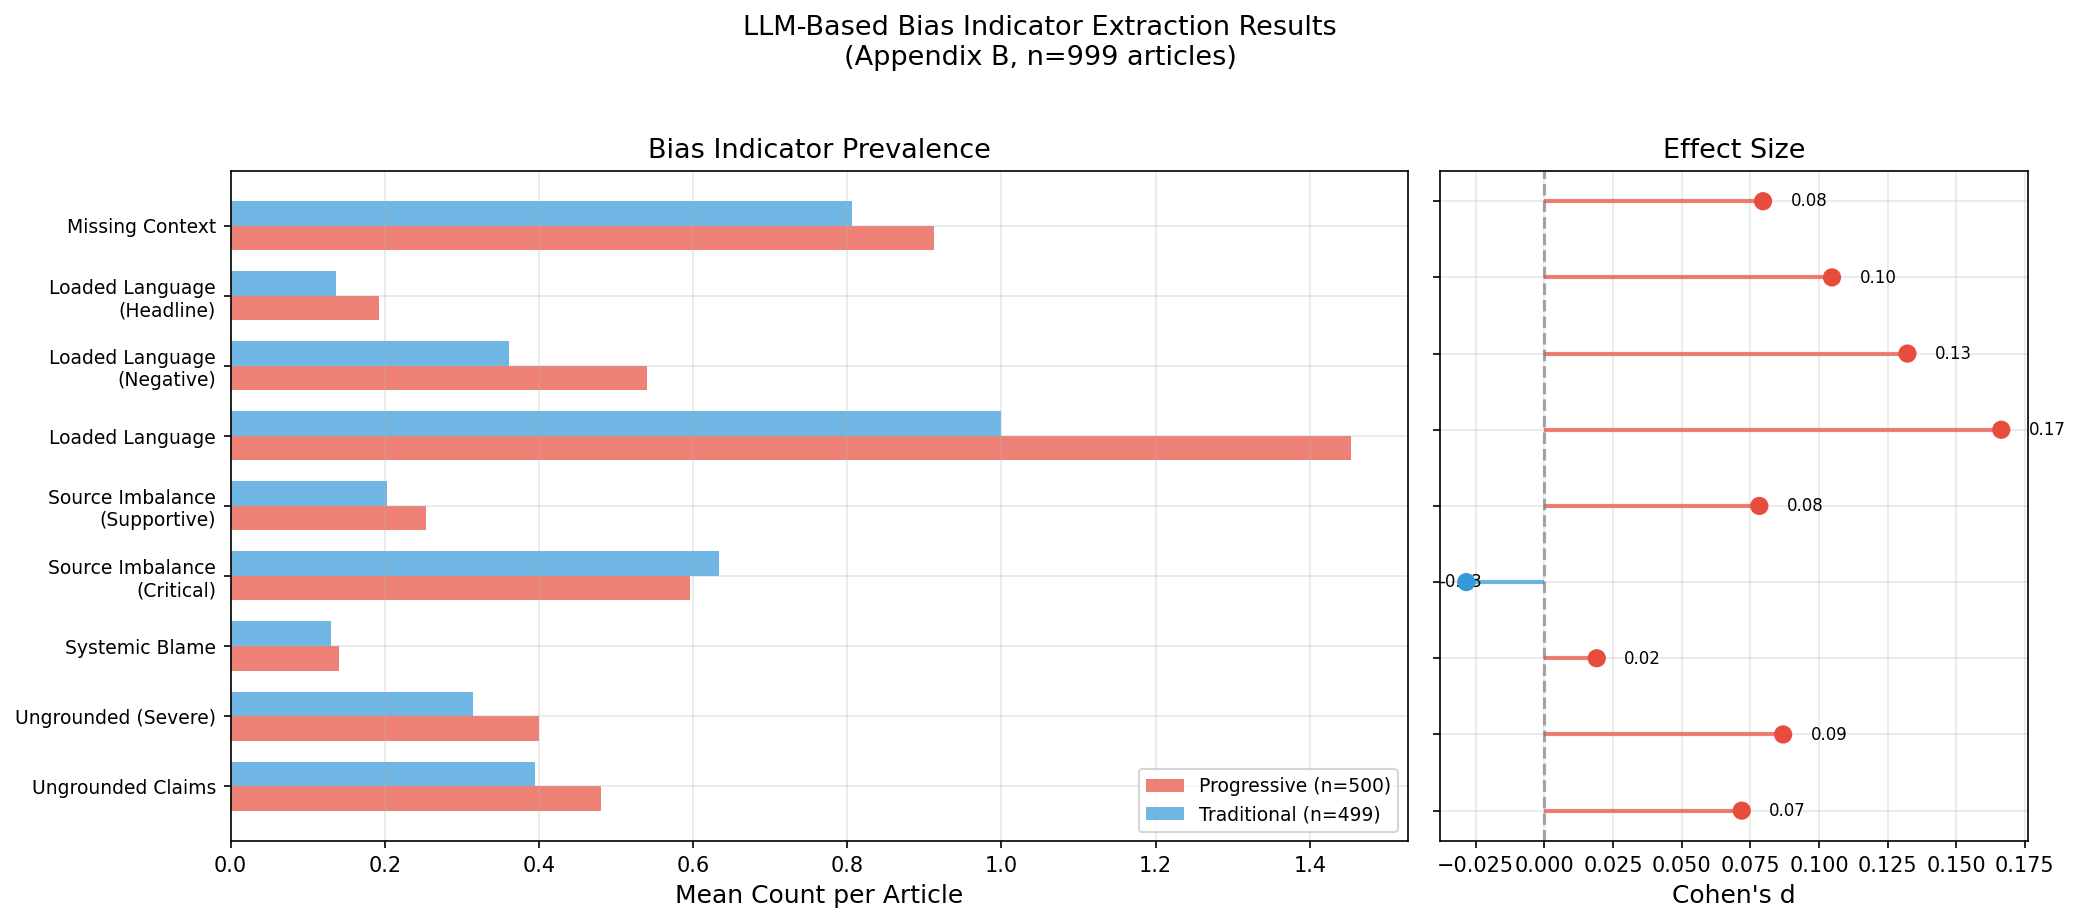
\includegraphics[width=0.95\textwidth]{09_bias_indicators.png}
  \caption{LLM-based bias indicator extraction results (Appendix B, $n = 999$). Left panel: mean indicator counts by ideology. Right panel: Cohen's $d$ effect sizes for each indicator. Loaded unfavorable language shows a modest differential toward progressive coverage ($d = +0.13$); the largest per-indicator effect is total loaded language ($d = +0.17$), while critical-source imbalance is near zero ($d = -0.03$).}
  \label{fig:biasindicators}
\end{figure}

\subsection*{Discussion}

The primary result is an affirmative equivalence rather than a mere null: at $n = 999$, the aggregate indicator-level asymmetry is bounded within $|d| < 0.2$ (TOST $p = .0055$) with a point estimate near zero ($d = -0.039$, $p = .541$). This contrasts with the significant $d = -0.151$ composite from the main pipeline (Section~4). The interpretation is that media bias toward progressive prosecutors operates through tone and framing, the aggregate evaluative register of coverage, rather than through discrete, identifiable journalistic violations (ungrounded claims, source imbalance, loaded language, missing context); at this sample size, that claim is a powered bound rather than a suggestive failure to detect.

An earlier version of this analysis, run before the valence revision, appeared to show a loaded-negative-language differential against progressive prosecutors and was read as a mechanistic bridge between the stance classifier's evaluative signal and a specific lexical practice. The corrected schema complicates that story rather than simply erasing it. In the 200-article re-extraction the differential appeared to vanish ($d = +0.01$); at $n = 999$ a modest loaded-unfavorable differential re-emerges ($0.54$ vs.\ $0.36$ per article, $d = +0.13$), alongside a smaller loaded-favorable differential ($d = +0.07$). These count differentials, however, do not produce net signed-score asymmetry --- the primary test is TOST-equivalent --- because the anti- and pro-prosecutor channels largely offset within the signed score. The strong mechanistic-bridge claim therefore remains withdrawn: progressive-prosecutor coverage contains somewhat more loaded language in \emph{both} directions, a volume difference rather than a directional lexical mechanism for the stance effect detected in Section~4. The moderate convergent validity ($r = 0.245$) between the two pipelines indicates that the bias score is tone-adjacent but measures a substantially distinct construct.

The within-county comparisons sharpen this picture. The San Francisco pair is statistically indistinguishable, but in Alameda, Price's coverage carries substantially more anti-prosecutor bias indicators than O'Malley's ($d = -0.433$, $p = .0095$). The overall equivalence thus masks offsetting county patterns, and the Alameda asymmetry coheres with the composite, stance, and controlled-ITS results, which likewise locate the robust effects in Alameda: discrete journalistic violations are not uniformly absent from the differential; they concentrate where the other instruments also detect it. At the same time, the per-prosecutor decomposition shows that prosecutors of both types attract indicator-dense coverage during politically contested periods (Jenkins's critical-source flags remain elevated), reinforcing the main paper's argument that bias detection requires multi-dimensional measurement: an approach sensitive only to explicit violations would miss the evaluative framing that drives the main effects, while an approach sensitive only to aggregate framing would miss the Alameda indicator asymmetry.

The analysis was upsized from a 200-article pilot to a stratified sample of 1{,}000 articles precisely to make the equivalence test and subgroup comparisons informative. The primary test is now well powered, though the Alameda paired comparison still rests on modest cells ($n = 66$ and $n = 119$, up from 11 and 28 in the pilot) and is one of two paired tests. All results reported in this appendix reflect the revised valence-aware schema and neutralized fictional-prosecutor exemplars described in the Method section; the original pilot schema, which lacked the valence attribute and used entity-keyed exemplars, produced results that did not survive the correction and are superseded.


% ────────────────────────────────────────────────────────────────────────
\section{Supplementary Diagnostic Figures and Tables}
\label{app:diagnostics}

This appendix consolidates diagnostic visuals and supporting tables moved from the main text for readability.

\begin{figure}[H]
  \centering
  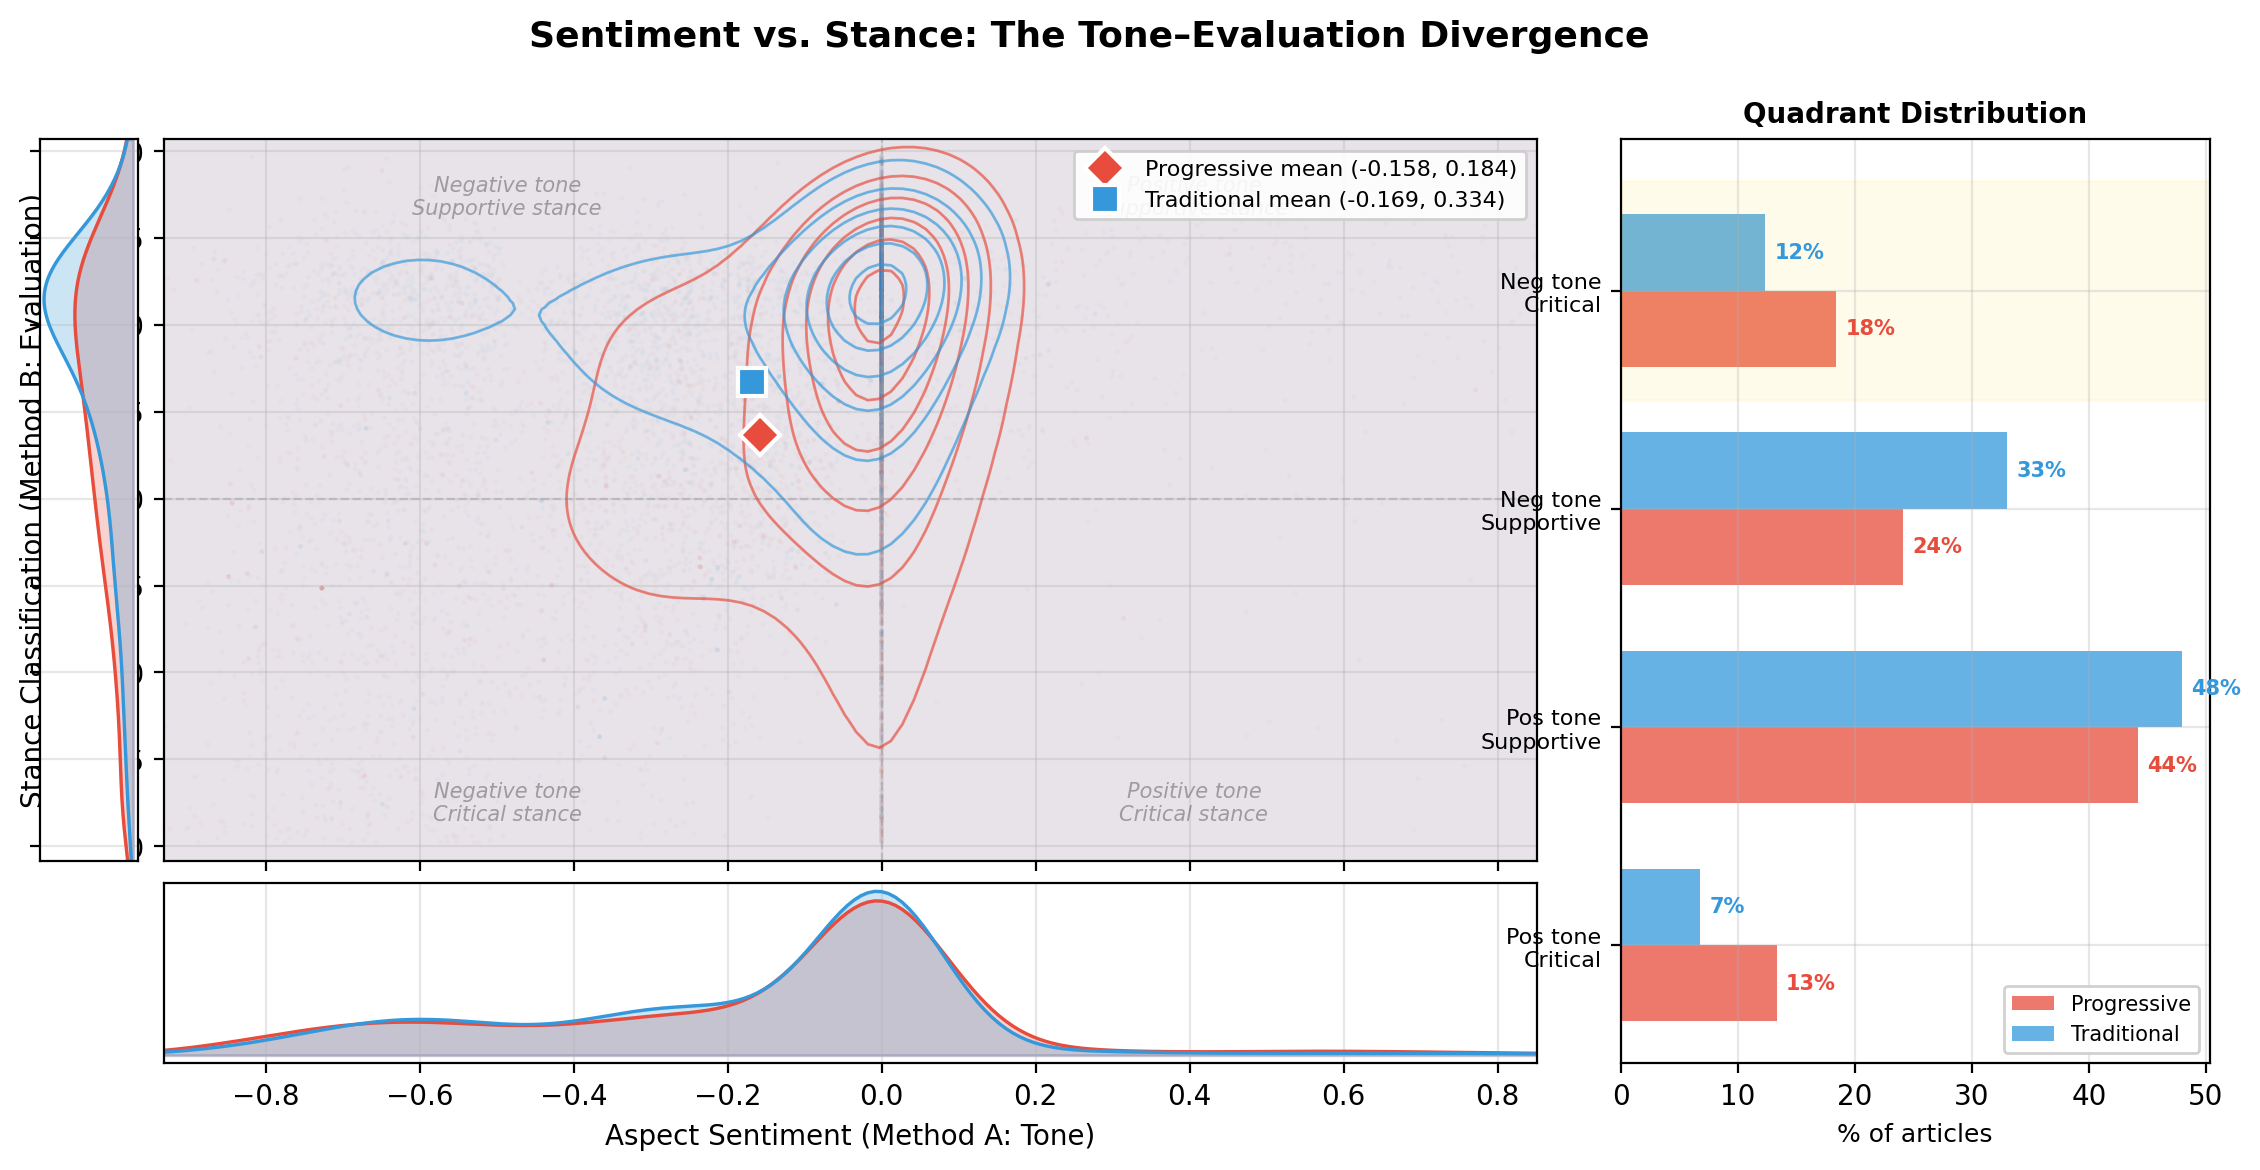
\includegraphics[width=0.95\textwidth]{10_method_comparison.png}
  \caption{Tone--evaluation divergence at the article level. Central panel: KDE contour plot of Method A (aspect sentiment) vs.\ Method B (stance classification) scores for progressive (red) and traditional (blue) prosecutors. The horizontal separation in stance contrasts with the overlapping sentiment distributions, confirming that media coverage differs in evaluative framing rather than emotional tone.}
  \label{fig:methodcomp}
\end{figure}

\begin{table}[ht]
\centering
\caption{Per-method OLS regressions: progressive prosecutor coefficient with cluster-robust SEs.}
\label{tab:methodreg}
\begin{tabular}{lrrrrr}
\toprule
Method & $\beta$ & $SE$ & $p$ & 95\% CI & $R^2$ \\
\midrule
B: Stance           & $\mathbf{-0.128}$ & 0.030 & $< .001$ & $[-0.187, -0.068]$ & .073 \\
C: Keywords          & $\mathbf{-0.010}$ & 0.002 & $< .001$ & $[-0.014, -0.006]$ & .053 \\
A: Aspect sentiment  & $0.010$           & 0.016 & $.507$   & $[-0.020, 0.041]$  & .010 \\
D: Document sentiment & $0.017$          & 0.013 & $.195$   & $[-0.009, 0.043]$  & .006 \\
\midrule
Composite            & $-0.021$          & 0.013 & $.104$   & $[-0.045, 0.004]$  & .023 \\
\bottomrule
\end{tabular}
\end{table}

\begin{figure}[H]
  \centering
  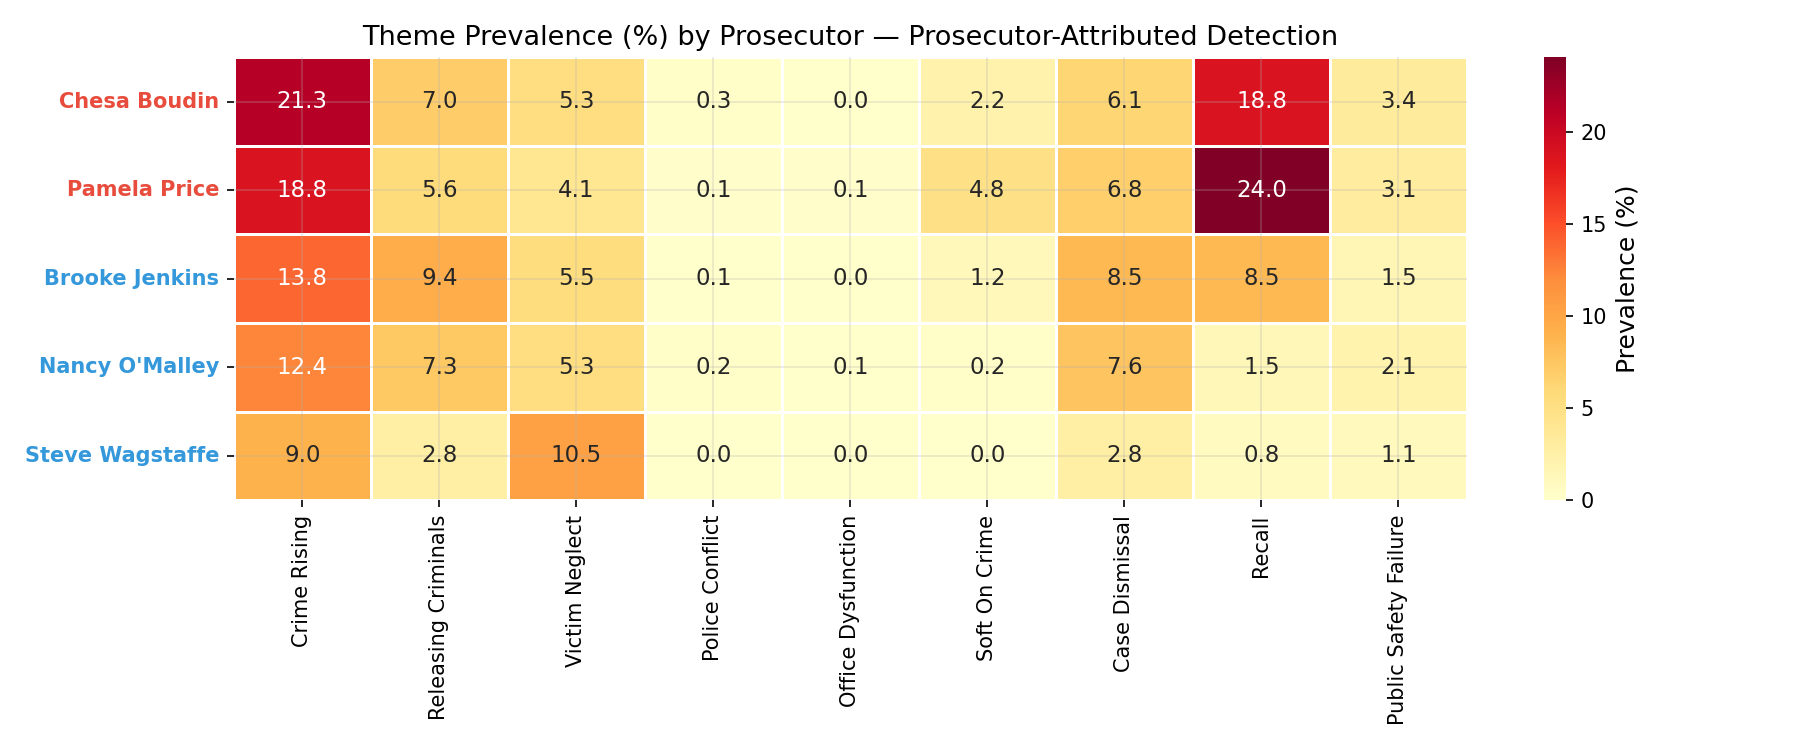
\includegraphics[width=\textwidth]{13_theme_attribution_heatmap.png}
  \caption{Theme prevalence (\%) by individual prosecutor. Rows are colored by ideology (red = progressive, blue = traditional). Darker cells indicate higher prevalence.}
  \label{fig:themeheat}
\end{figure}

\begin{figure}[H]
  \centering
  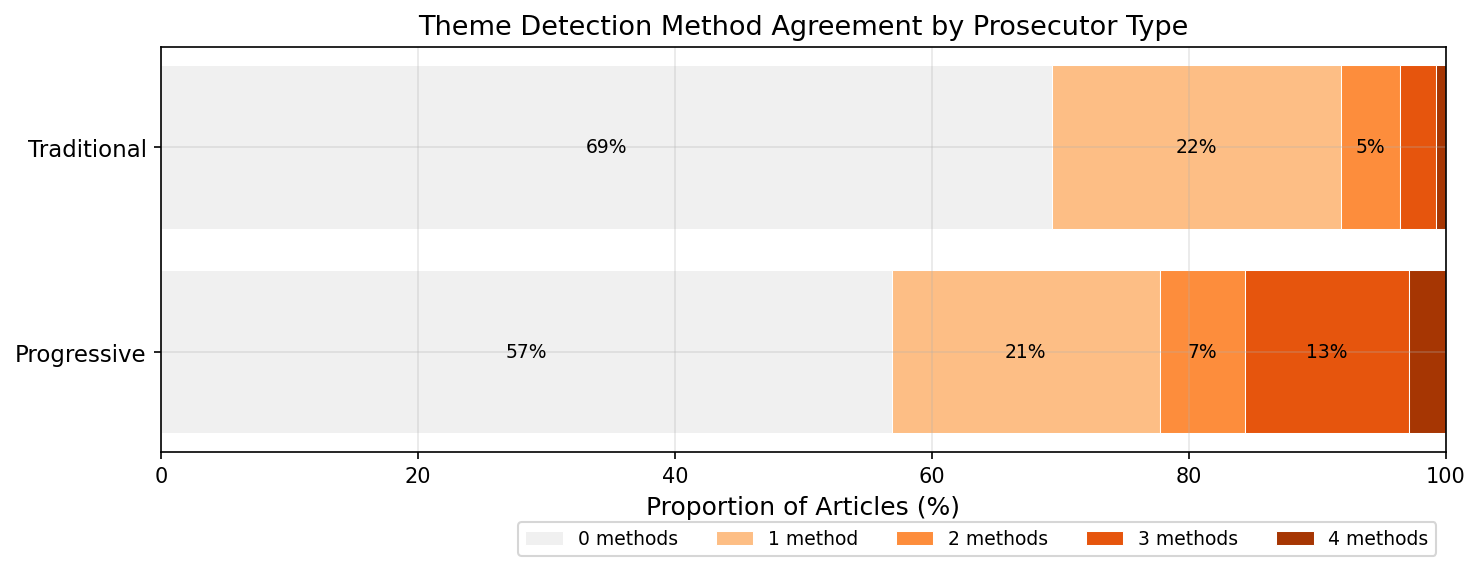
\includegraphics[width=0.85\textwidth]{14_theme_method_agreement.png}
  \caption{Distribution of detection method agreement by prosecutor type. Segments show the proportion of articles detected by 0--4 independent methods.}
  \label{fig:themeagree}
\end{figure}

\section{Illustrative Examples of Identified Bias by Method}
\label{app:examples}

This appendix presents concrete examples from the corpus to illustrate what each method detects. Examples are drawn from articles at the extremes of each method's score distribution and are intended to make the abstract measurement pipeline tangible.

\subsection*{Method A: Aspect-Based Sentiment Analysis}

Method A extracts three-sentence context windows around prosecutor mentions. The following window scored $A = -0.932$ (\emph{San Francisco Chronicle}, about Pamela Price):

\begin{quote}
``Don't blame Alameda DA Price for crime. The pandemic changed everything, and we failed low-opportunity communities, especially our youth; crime in our cities has climbed in some areas and it is frightening.''
\end{quote}

Although the article's argument is \emph{defensive} of Price, the RoBERTa model responds to the emotional valence of surrounding language, including ``crime,'' ``climbed,'' and ``frightening,'' rather than the argumentative intent. By contrast, a reader letter produced $A = +0.955$: ``I am so thankful for Alameda County District Attorney Pamela Price. She has taken on an enormous job and she is doing it well.''

\subsection*{Method B: Zero-Shot Stance Classification}

A paragraph from kron4.com received a critical stance score of $B = -0.996$:

\begin{quote}
``[The letter] cites failed leadership, the movement to defund the police and the district attorney's unwillingness to charge and prosecute people who commit life threatening crimes.''
\end{quote}

BART-MNLI classifies this as criticizing the prosecutor's handling of crime with near-certainty. The divergence between Methods A and B ($d = 0.047$ for sentiment vs.\ $d = -0.337$ for stance) is visible in individual examples: an article can score near zero on sentiment while scoring highly critical on stance.

\subsection*{Method C: Enhanced Keyword Analysis}

An article about Nancy O'Malley (berkeleyside.org) triggered three themes simultaneously: \textbf{soft-on-crime} (``very \textbf{light sentences} or no sentences at all''), \textbf{releasing criminals} (``Boudin has \textbf{released} a person accused of a crime''), and \textbf{recall} (``announced a \textbf{recall campaign} against O'Malley''). The keywords capture thematic framing rather than sentiment: ``light sentences'' is emotionally neutral but thematically codes the soft-on-crime narrative.

\subsection*{Method D: Document-Level Sentiment}

Because crime reporting is inherently negative, Method D reveals a paradoxical pattern: articles about traditional prosecutors are slightly \emph{more} negative in overall tone ($d = +0.049$, $p = .005$). This underscores why prosecutor-specific methods are necessary.

\subsection*{Media Framing Analysis}

The framing analysis classifies paragraphs (including standalone headlines) into five narrative frames. Illustrative examples include:

\begin{table}[ht]
\centering
\small
\caption{Illustrative examples of each dominant media frame (Appendix C).}
\begin{tabularx}{\textwidth}{lXlr}
\toprule
Frame & Example Headline & Prosecutor & Score \\
\midrule
Accountability & ``SF DA Boudin Blamed by Some for Release of Parolee\ldots'' & Boudin & 1.00 \\
Conflict & ``Jenkins blames Boudin in decision to drop case\ldots'' & Jenkins & 1.00 \\
Human interest & ``Family of woman killed in S.F.\ New Year's hit and run\ldots'' & Boudin & 1.00 \\
Reform & ``As new D.A., Jenkins vows to be tougher than Boudin'' & Jenkins & 1.00 \\
Consequences & ``Price's office lags on providing charging data'' & Price & 0.99 \\
\bottomrule
\end{tabularx}
\end{table}

Progressive prosecutors are nearly twice as likely to receive accountability framing (41.1\% vs.\ 24.6\%) and more than three times more likely to receive reform framing (4.2\% vs.\ 1.2\%), while traditional prosecutors receive substantially more human-interest coverage (33.6\% vs.\ 21.4\%; see also Figure~\ref{fig:heatmap}).

\subsection*{Prosecutor-Attributed Theme Detection}

The theme attribution method ($d = -0.42$) requires anti-prosecutor themes to be explicitly linked to a named prosecutor through compound linguistic patterns, distinguishing it from the proximity-based keyword method (Method~C). An article titled ``Boudin Blunders: SF DA's downfall leading up to recall'' (\emph{kron4.com}, 2022-06-08) received the corpus's highest theme attribution score (21.3), with four independent detection methods identifying themes including crime-rising, soft-on-crime, case-dismissal, recall, and public-safety-failure. By contrast, a routine crime article about a man accused of hitting a woman with a car (\emph{San Mateo Daily Journal}, 2021-09-24) attributed to Wagstaffe received a theme score of 0.0, illustrating the method's specificity in not flagging ordinary crime coverage merely because a prosecutor is mentioned.

\subsection*{LLM-Based Bias Indicator Detection}

A \emph{Mission Local} article about District Attorney Jenkins's handling of the Keita O'Neil case (2023-03-07) produced 22 bias indicators, including \textbf{loaded language} (``killer cops'' as pejorative label; ``swept under the rug of political expediency'' as ideological framing), \textbf{source imbalance} (extended critical quotes from the victim's family and their attorney with no counterbalance), and \textbf{missing context} (the prosecutorial rationale for dismissing the charges is never presented). Critically, a large share of the sampled articles (428 of 999, 43\%) produce zero indicators: evidence-based critical reporting is not flagged as biased. The method also detects bias \emph{favoring} prosecutors, supporting the finding that bias is not unidirectional.

\section{Sensitivity to Traditional Baseline Composition}
\label{app:baseline_sensitivity}

Brooke Jenkins accounts for roughly half of the traditional baseline ($n=3{,}097$ of $n=\NTradAttributed$ traditional articles). Because this can attenuate pooled traditional estimates, I recomputed group comparisons after excluding Jenkins and retaining all progressive articles ($n=\NoJenkinsNProg$ progressive; $n=\NoJenkinsNTrad$ traditional).

\begin{table}[H]
\centering
\caption{Per-method sensitivity to excluding Brooke Jenkins from the traditional baseline.}
\label{tab:baseline_sensitivity}
\begin{tabular}{lcc}
\toprule
Outcome & Full sample ($d$, $p$) & Excluding Jenkins ($d$, $p$) \\
\midrule
Composite & $d=\FullCompositeD$, $p=\FullCompositeP$ & $d=\NoJenkinsCompositeD$, $p=\NoJenkinsCompositeP$ \\
Stance & $d=\FullStanceD$, $p=\FullStanceP$ & $d=\NoJenkinsStanceD$, $p=\NoJenkinsStanceP$ \\
Keywords & $d=\FullKeywordsD$, $p=\FullKeywordsP$ & $d=\NoJenkinsKeywordsD$, $p=\NoJenkinsKeywordsP$ \\
Aspect sentiment & $d=\FullAspectD$, $p=\FullAspectP$ & $d=\NoJenkinsAspectD$, $p=\NoJenkinsAspectP$ \\
Document sentiment & $d=\FullDocD$, $p=\FullDocP$ & $d=\NoJenkinsDocD$, $p=\NoJenkinsDocP$ \\
\bottomrule
\end{tabular}
\end{table}

Excluding Jenkins strengthens the composite, stance, and keyword differentials materially, while sentiment metrics remain small and comparatively weak. This indicates that full-sample estimates are conservative with respect to evaluative dimensions.

For the complementary robustness check that removes fallback-attributed articles instead of a specific prosecutor baseline component, see Appendix~\ref{app:fallback_sensitivity}.

\section{Sample-Composition Sensitivity Analyses}
\label{app:fallback_sensitivity}

In the attribution pipeline, fallback assignments occur when an article contains generic DA references (e.g., ``the district attorney'') but no named prosecutor mention; in these cases, the article is assigned by publication county and article date. This mechanism expands coverage but can introduce measurement noise when outlets report cross-county stories.

Using the article-level analysis sample from Section~4 ($n=\NoFallbackNTotal$), fallback assignment accounts for $\NoFallbackExcludedN$ articles (\NoFallbackExcludedPct\%). Excluding these fallback-attributed cases leaves $\NoFallbackRemainingN$ directly attributed articles (named-mention based), with $n=\NoFallbackNProg$ progressive and $n=\NoFallbackNTrad$ traditional.

\begin{table}[H]
\centering
\caption{Composite group comparison: full sample vs.\ sample-composition sensitivities.}
\label{tab:fallback_sensitivity}
\begin{tabular}{lrrrrrr}
\toprule
Sample & $n_{\text{Prog}}$ & $M_{\text{Prog}}$ & $n_{\text{Trad}}$ & $M_{\text{Trad}}$ & $d$ & $p_{\text{Welch}}$ \\
\midrule
Full attributed sample & \NProgAttributed & $-0.0304$ & \NTradAttributed & $-0.0020$ & $\FullCompositeD$ & $\FullCompositeP$ \\
Exclude fallback-assigned & \NoFallbackNProg & $-0.0385$ & \NoFallbackNTrad & $+0.0213$ & $\NoFallbackCompositeD$ & $\NoFallbackCompositeP$ \\
Prosecutor-focused subsample & 2{,}209 & $-0.0432$ & 1{,}790 & $+0.0052$ & $-0.260$ & $1.1\times 10^{-16}$ \\
Mention-dominance subsample & 2{,}043 & $-0.0429$ & 1{,}738 & $+0.0068$ & $-0.267$ & $1.3\times 10^{-16}$ \\
Tenure-period only & 6{,}314 & $-0.0378$ & 6{,}234 & $-0.0020$ & $-0.192$ & $8.8\times 10^{-27}$ \\
\bottomrule
\end{tabular}
\end{table}

The no-fallback estimate is approximately double the full-sample effect size in magnitude. The bootstrap mean difference (progressive minus traditional) is $\NoFallbackBootDiff$ with 95\% CI $[\NoFallbackBootCiLo,\ \NoFallbackBootCiHi]$, confirming that the progressive group remains significantly more negative after removing all fallback assignments. Substantively, this indicates that fallback attribution is conservative in this corpus: it attenuates the ideology differential rather than driving it.

Three further sample-composition sensitivities, motivated by the human validation audit (Section~\ref{sec:human_validation}), probe attribution quality from complementary directions. First, a \emph{prosecutor-focused} subsample retains an article only if it mentions the primary prosecutor at least twice by name or mentions the prosecutor in the headline. This rule was validated against the research-assistant-coded benchmark, where it separated the 28 low-relevance articles in the 100-article validation sample with 100\% recall and precision (a continuous weighted centrality score achieves AUC $= 0.90$). Graded against the larger pooled benchmark now available---the 57 low-relevance and wrong-target articles the research assistant flagged across the first three validation packets, among 333 distinct coded articles---the rule drops 72\% of flagged articles while 91\% of the articles it retains are genuinely prosecutor-focused. Its residual failures are articles that name the attributed prosecutor repeatedly while actually being about another prosecutor, so the subsample retains some peripheral coverage. The rule keeps 3{,}999 of 12{,}827 articles, and the composite differential increases to $d = -0.260$ ($p = 1.1\times 10^{-16}$). Like the fallback exclusion, this indicates that articles genuinely centered on the attributed prosecutor exhibit a larger differential than the full attributed sample.

Second, a \emph{mention-dominance} subsample tightens the same relevance logic to address that residual failure mode. The pooled flags show that the misses concentrate in articles about a different prosecutor, usually a reform prosecutor outside the study: Gasc\'{o}n, Harris, or Rosen is named in 20 of the 57 flagged articles. The mention-dominance rule therefore requires, in addition to the mentions-or-headline condition, that the primary prosecutor be named more often than all other prosecutors combined, counting both the study's other four and prominent non-study prosecutors (Gasc\'{o}n, Harris, Rosen, Spitzer, Chisholm, Krasner, Mosby, and Foxx). This raises performance to 84\% of flagged articles dropped at 94\% precision, with no cost on the packet-01 benchmark, where both rules separate the 28 low-relevance articles perfectly. The rule keeps 3{,}781 of 12{,}827 articles, and the composite differential is $d = -0.267$ ($p = 1.3\times 10^{-16}$). One caveat is essential and limits what this estimate establishes: the dominance rule was developed using the same flags it is graded against, so the evaluation is in-sample, and out-of-sample confirmation with the second blinded coder is pending. The reported gain over the simpler rule should be read as an upper bound on what the added condition buys, not as a validated improvement.

The three relevance-based restrictions converge. Excluding fallback assignments ($d = -0.294$), restricting to prosecutor-focused articles ($d = -0.260$), and applying the mention-dominance rule ($d = -0.267$) each roughly double the full-sample effect ($d = -0.151$) in the same direction, despite selecting overlapping but distinct subsamples by different criteria. Restricting the corpus to coverage genuinely about the attributed prosecutor strengthens rather than weakens the contrast, the pattern expected if peripheral and misattributed articles contribute noise centered near zero rather than generating the differential.

Third, a \emph{tenure-period-only} sample excludes the 279 articles published before the attributed prosecutor took office, most of which are campaign coverage (208 concern Boudin's 2019 campaign). The composite differential is essentially unchanged and slightly strengthened ($d = -0.192$, $p = 8.8\times 10^{-27}$), indicating that pre-tenure campaign coverage does not drive the main result.

\section{Segmented Interrupted Time-Series Robustness}
\label{app:segmented_its}

The main text reports a concise segmented ITS summary for temporal dynamics by method. This appendix provides the full model specification, coefficient table, and plots for those temporal analyses:
\[
Y_t = \beta_0 + \beta_1 t + \beta_2 \text{Post}_t + \beta_3 \text{TimeAfter}_t + \varepsilon_t
\]
where $\beta_2$ captures an immediate level shift at transition and $\beta_3$ captures post-transition slope change. The transition month itself is coded as the first post-transition month ($\text{TimeAfter}=0$ in that month), so $\beta_2$ is the level change at the first month of the new prosecutor's tenure. Models are weighted by monthly article counts and use Newey--West (HAC) robust standard errors.

\begin{table}[H]
\centering
\caption{Segmented ITS results (monthly, weighted, HAC-robust).}
\label{tab:segmented_its}
\begin{tabular}{llccc}
\toprule
Transition & Outcome & Level shift $\beta_2$ & Slope change $\beta_3$ & 12-month net effect \\
\midrule
SF (Boudin $\rightarrow$ Jenkins) & Composite & $\SFItsCompLevelBeta$ ($p\SFItsCompLevelP$) & $\SFItsCompSlopeBeta$ ($p\SFItsCompSlopeP$) & $\SFItsCompEffectTwelveM$ ($p\SFItsCompEffectP$) \\
SF (Boudin $\rightarrow$ Jenkins) & Stance & $\SFItsStanceLevelBeta$ ($p\SFItsStanceLevelP$) & $\SFItsStanceSlopeBeta$ ($p\SFItsStanceSlopeP$) & $\SFItsStanceEffectTwelveM$ ($p\SFItsStanceEffectP$) \\
SF (Boudin $\rightarrow$ Jenkins) & Keywords & $\SFItsKeywordsLevelBeta$ ($p\SFItsKeywordsLevelP$) & $\SFItsKeywordsSlopeBeta$ ($p\SFItsKeywordsSlopeP$) & $\SFItsKeywordsEffectTwelveM$ ($p\SFItsKeywordsEffectP$) \\
\midrule
Alameda (O'Malley $\rightarrow$ Price) & Composite & $\AlItsCompLevelBeta$ ($p\AlItsCompLevelP$) & $\AlItsCompSlopeBeta$ ($p\AlItsCompSlopeP$) & $\AlItsCompEffectTwelveM$ ($p\AlItsCompEffectP$) \\
Alameda (O'Malley $\rightarrow$ Price) & Stance & $\AlItsStanceLevelBeta$ ($p\AlItsStanceLevelP$) & $\AlItsStanceSlopeBeta$ ($p\AlItsStanceSlopeP$) & $\AlItsStanceEffectTwelveM$ ($p\AlItsStanceEffectP$) \\
Alameda (O'Malley $\rightarrow$ Price) & Keywords & $\AlItsKeywordsLevelBeta$ ($p\AlItsKeywordsLevelP$) & $\AlItsKeywordsSlopeBeta$ ($p\AlItsKeywordsSlopeP$) & $\AlItsKeywordsEffectTwelveM$ ($p\AlItsKeywordsEffectP$) \\
\bottomrule
\end{tabular}
\end{table}

Figure~\ref{fig:segmented_its} visualizes the same segmented models for the three most policy-relevant outcomes (composite, stance, keywords), plotting observed monthly means and fitted segmented trends around each transition date.

\begin{figure}[H]
\centering
  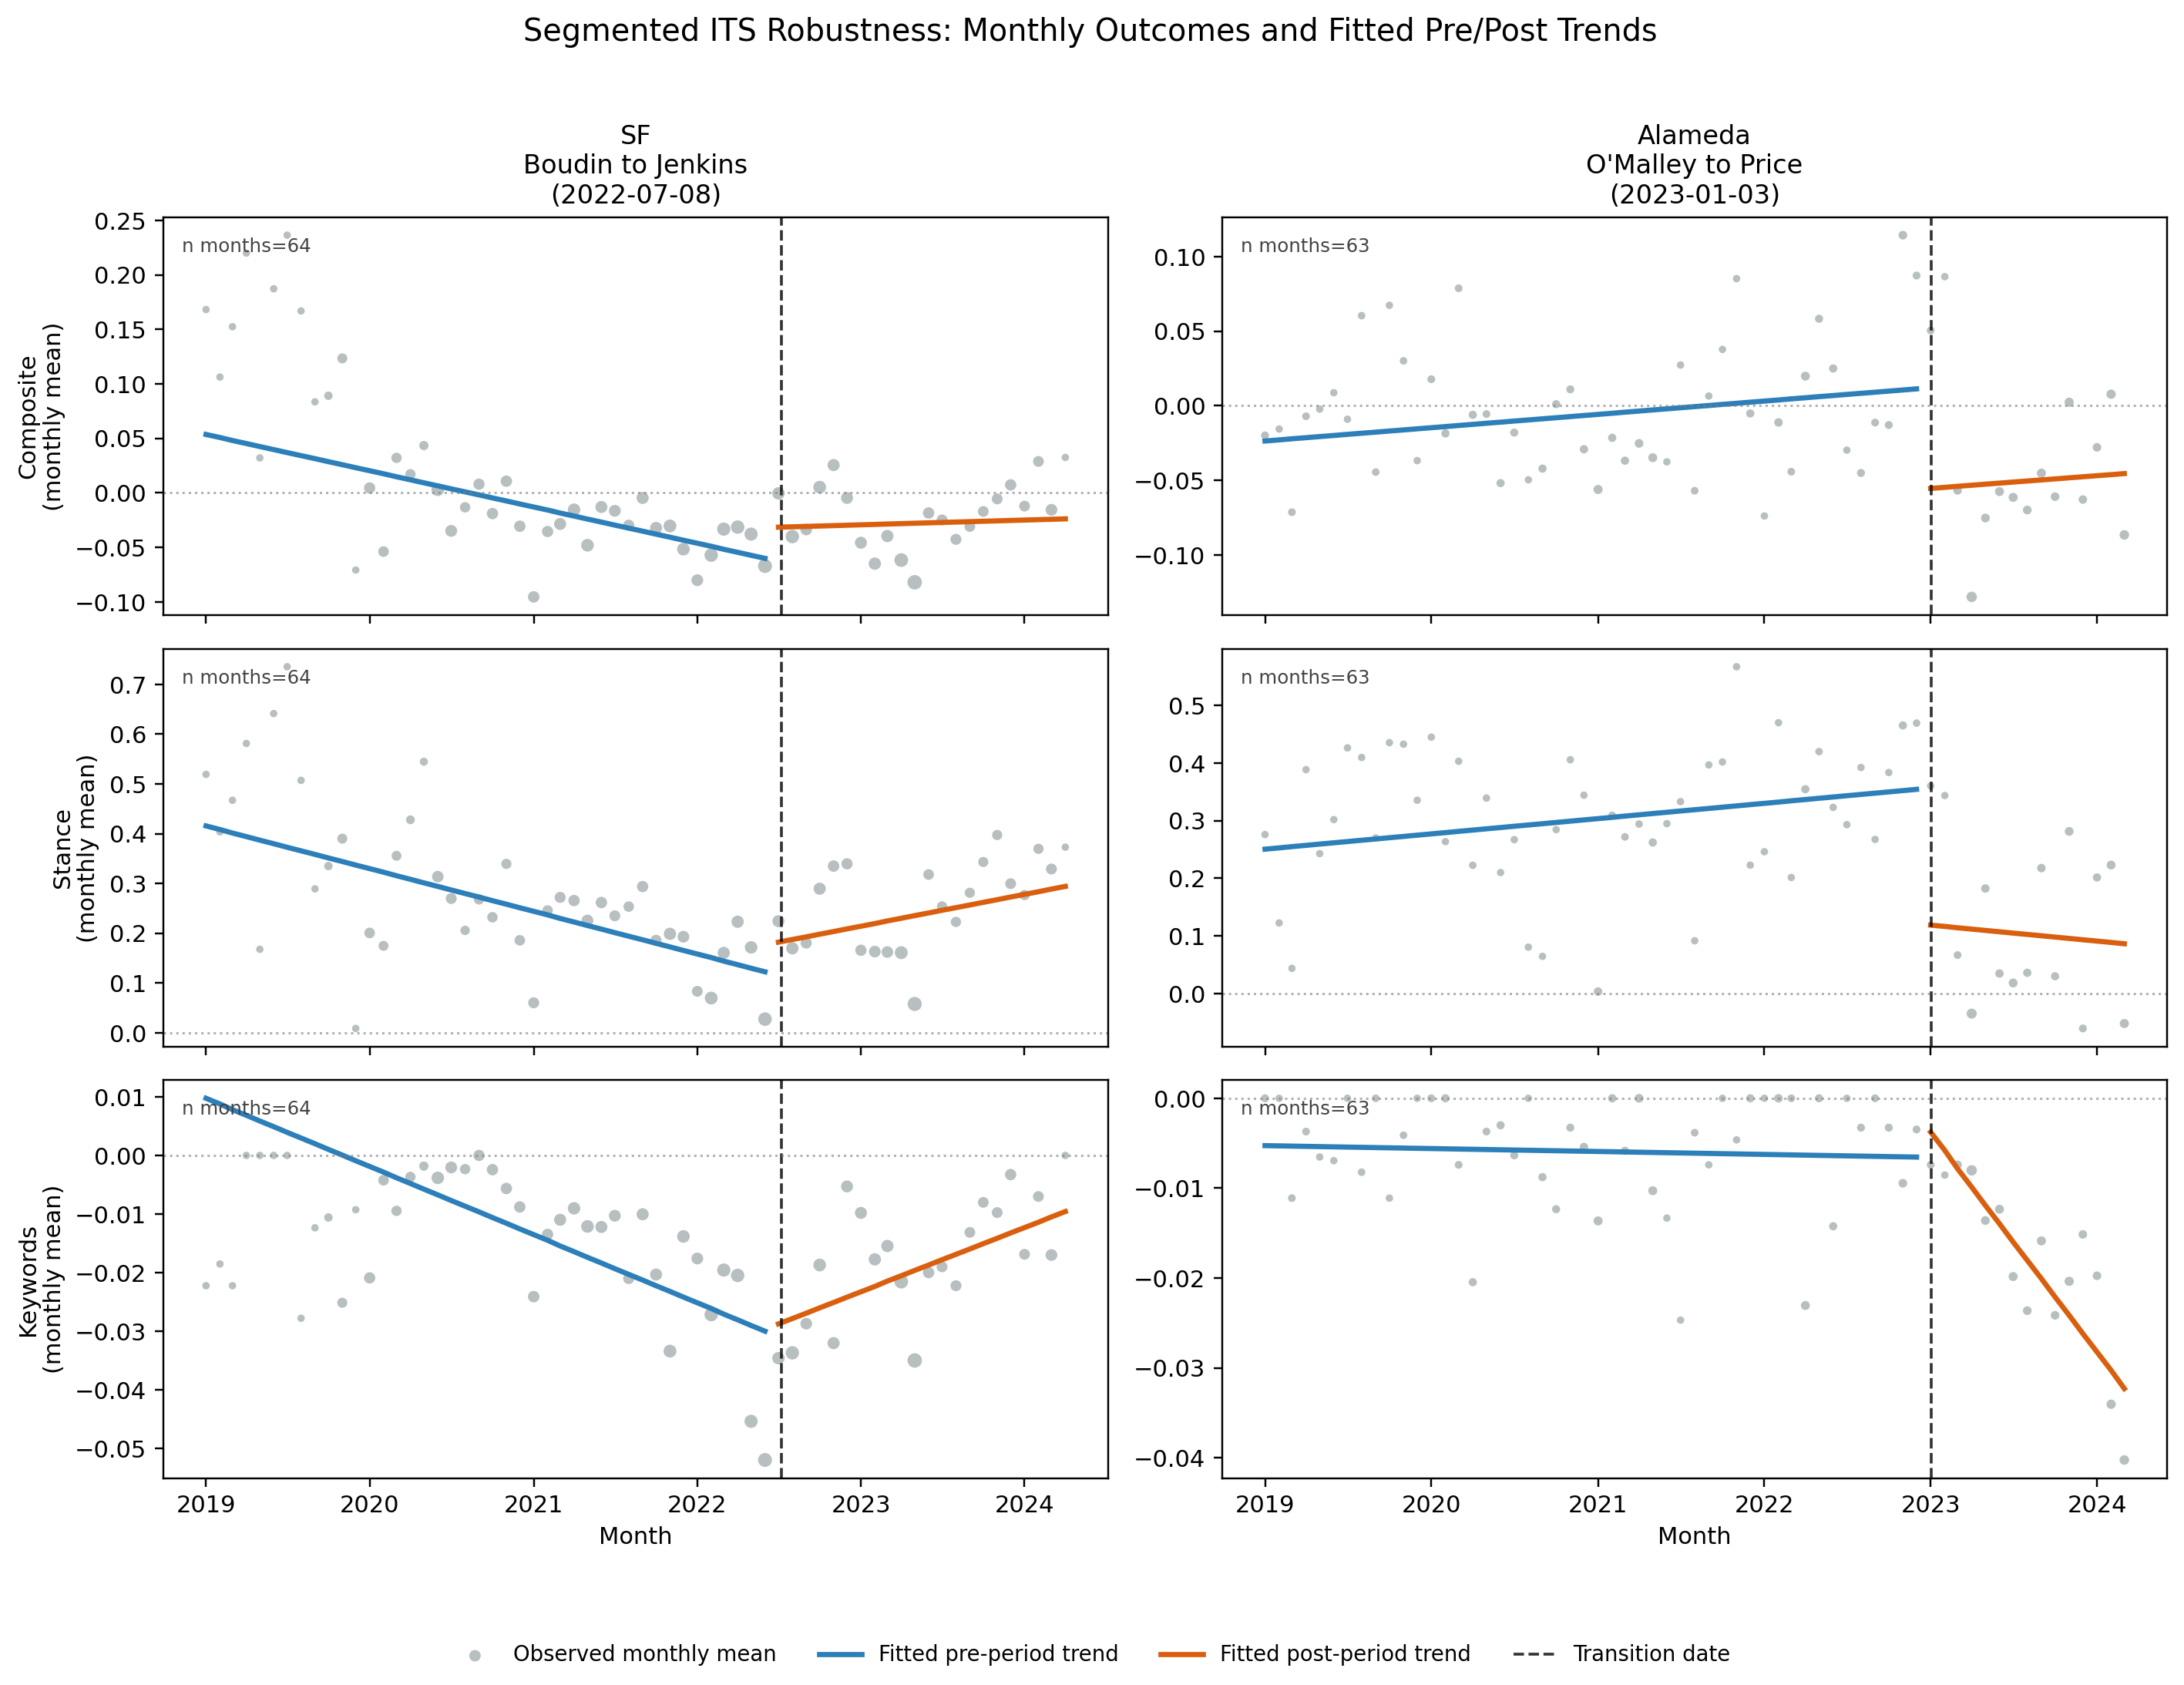
\includegraphics[width=\textwidth]{18_segmented_its.png}
  \caption{Segmented ITS robustness plots. Points are monthly outcome means (marker size proportional to monthly article count). Colored lines are fitted segmented trends before and after transition; dashed vertical lines mark transition dates.}
  \label{fig:segmented_its}
\end{figure}

These segmented models sharpen interpretation by separating immediate transition shifts from post-transition trend changes. In San Francisco, the composite shows a modest positive level shift that does not reach significance ($p = .070$) and a nominally significant positive post-transition slope, consistent with movement toward less negative coverage after the Boudin-to-Jenkins transition. In Alameda, the composite shows a nominally significant immediate negative level shift at the Price transition with no significant slope change, consistent with a step increase in negative coverage. Across both transitions, stance remains the strongest and most consistent evaluative signal.

Because the segmented models involve a 30-test family (two transitions $\times$ five outcomes $\times$ three quantities: level change, slope change, and 12-month horizon effect), Benjamini--Hochberg adjusted $p$-values are computed across the full family (replication output \texttt{12\_segmented\_its\_table.csv}). The adjustment changes several conclusions. The San Francisco composite level shift is not significant even before correction ($p = .070$); under the earlier, time-asymmetric attribution filter this coefficient had appeared nominally significant, and its disappearance under the corrected attribution is expected, because the 126 removed post-tenure false positives were concentrated precisely in the post-transition window (see the attribution discussion in the Data and Methods section). The San Francisco composite slope change ($p = .031$, $p_{BH} = .078$), the Alameda composite level shift ($p = .035$, $p_{BH} = .080$), and the Alameda composite 12-month horizon effect ($p = .030$, $p_{BH} = .078$) are no longer significant after correction and should be treated as suggestive rather than confirmed. The effects that survive correction are concentrated in the evaluative components. In San Francisco: the stance slope change ($p_{BH} = .002$) and 12-month effect ($p_{BH} < .001$), the keyword slope change ($p_{BH} = .001$) and 12-month effect ($p_{BH} = .032$), and the composite 12-month horizon effect ($p_{BH} = .002$). In Alameda: the stance level shift ($p_{BH} = .002$) and 12-month effect ($p_{BH} < .001$), and the keyword slope change and 12-month effect (both $p_{BH} < .001$). No sentiment-outcome test survives correction. The family-wise-robust conclusion from the ITS analysis is therefore about the evaluative channels, not the composite: transition-linked shifts in stance and keyword salience are reliable, while the composite-level step changes are not separately established.

As a further check against region-wide trends, I re-estimate the segmented models on a controlled difference series: each treated county's monthly outcome minus the contemporaneous monthly outcome for San Mateo County (Steve Wagstaffe), an untreated comparison county that experienced no prosecutor transition over the study period. In this controlled specification, the San Francisco composite level shift is no longer distinguishable from contemporaneous county-general trends ($\beta_2 = +0.028$, $p = .26$; the controlled San Francisco stance level shift is likewise non-significant, $p = .096$), suggesting that part of the San Francisco pattern reflects Bay Area-wide movement in crime-news coverage. The Alameda composite level shift, by contrast, survives the control and sharpens ($\beta_2 = -0.087$, $p = .003$), with the stance outcome showing the same pattern ($\beta_2 = -0.242$, $p < .001$); the step increase in negative Alameda coverage at the Price transition therefore cannot be attributed to region-wide shifts in coverage tone. The controlled contrast is a separate, pre-specified single comparison per county rather than part of the 30-test uncontrolled family, so it is not folded into the Benjamini--Hochberg adjustment above; read together, the two analyses agree that the Alameda transition effect is the more reliable one, carried by the stance channel (which survives family-wise correction) and confirmed against the untreated county, while the San Francisco composite-level results are suggestive under both lenses. These robustness analyses improve temporal identification but should still be interpreted descriptively: the controlled contrast relies on a single comparison county and cannot rule out county-specific confounds.

\end{appendices}

\end{document}
